\documentclass[10pt]{article}
\usepackage[utf8]{inputenc}
\usepackage[T1]{fontenc}
\usepackage{amsmath}
\usepackage{amsfonts}
\usepackage{amssymb}
\usepackage{mhchem}
\usepackage{stmaryrd}
\usepackage{mathrsfs}
\usepackage{bbold}
\usepackage{graphicx}
\usepackage[export]{adjustbox}
\graphicspath{ {./images/} }

\title{Chapter 16 }

\author{}
\date{}


\begin{document}
\maketitle
\section{Non-Stationary Time Series}
\subsection{Introduction}
At the beginning of Chapter 14 we displayed a set of economic time series. Several (real GDP, exchange rate, interest rate, crude oil price) did not appear to be stationary. In Section $14.23$ we introduced the non-stationary unit root process which is an autoregressive process with an autoregressive root at unity. Plots of two simulated examples (Figure 14.5) displayed time-paths with wandering behavior similar to the economic time series. This suggests that perhaps a unit root autoregression is a reasonable model for these series. In this chapter we explore econometric estimation and inference for non-stationary unit root time series.

\subsection{Partial Sum Process and Functional Convergence}
Take the multivariate random walk
$$
Y_{t}=Y_{t-1}+e_{t}
$$
where $\left(e_{t}, \mathscr{F}_{t}\right)$ is a vector MDS with finite covariance matrix $\Sigma$. By back-substitution we find $Y_{t}=Y_{0}+S_{t}$ where
$$
S_{t}=\sum_{i=1}^{t} e_{i}
$$
is the cumulative sum of the errors up to time $t$. We call $S_{t}$ a partial sum process.

The time index $t$ ranges from 0 to $n$. Write ${ }^{1} t=\lfloor n r\rfloor$ as a fraction $r$ of the sample size $n$. This allows us to write $S_{\lfloor n r\rfloor}$ as a function of the fraction $r$. Divide by $\sqrt{n}$ so that the variance is stabilized. With these modifications we define the standardized partial sum process.
$$
S_{n}(r)=\frac{1}{\sqrt{n}} S_{\lfloor n r\rfloor}=\frac{1}{\sqrt{n}} \sum_{t=1}^{\lfloor n r\rfloor} e_{t} .
$$
The random process $S_{n}(r)$ is a scaled version of the time-series $Y_{t}$ and is a function of the sample fraction $r \in[0,1]$. It is a stochastic process meaning that it is a random function. For any finite $n, S_{n}(r)$ is a step function with $n$ jumps.

Let's consider the behavior of $S_{n}(r)$ as $n$ increases. It's largest discrete jump equals $n^{-1 / 2} \max _{1 \leq t \leq n}\left\|e_{t}\right\|$. Theorem $6.15$ shows that this is $o_{p}(1)$. This suggests that the jumps in $S_{n}(r)$ asymptotically vanish. We would like to find its asymptotic distribution. We expect the limit distribution to be a stochastic process as well.

${ }^{1}$ The notation $\lfloor x\rfloor$ means "round down to the nearest integer". To do so we need to define the asymptotic distribution of a random function. The primary tool is the functional central limit theorem (FCLT) which is a component of empirical process theory (Chapter 18 of Probability and Statistics for Economists). It turns out that the FCLT depends on how we measure the difference between two functions. The most commonly used measure is the uniform metric. On the space of functions from $[0,1]$ to $\mathbb{R}^{m}$ it is
$$
\rho\left(v_{1}, v_{2}\right)=\sup _{0 \leq r \leq 1}\left\|v_{1}(r)-v_{2}(r)\right\| .
$$
Convergence in distribution for random processes (e.g. Definition $18.6$ of Probability and Statistics for Economists) is defined with respect to a specific metric. While we don't repeat the details here the important consequence is that continuity is defined with respect to this metric and this impacts applications such as the continuous mapping theorem.

The Functional Central Limit Theorem (Theorem $18.9$ of Probability and Statistics for Economists) states that $S_{n}(r) \underset{d}{\longrightarrow} S(r)$ as a function over $r \in[0,1]$ if two conditions hold:

\begin{enumerate}
  \item The limit distributions of $S_{n}(r)$ coincide with those of $S(r)$.

  \item $S_{n}(r)$ is asymptotically equicontinuous.

\end{enumerate}
The first condition means that for any fixed $r_{1}, \ldots, r_{m},\left(S_{n}\left(r_{1}\right), \ldots, S_{n}\left(r_{m}\right)\right) \underset{d}{\longrightarrow}\left(S\left(r_{1}\right), \ldots, S\left(r_{m}\right)\right)$. The second condition is technical but essentially requires that $S_{n}(r)$ is approximately continuous with respect to the uniform metric in large samples.

We now characterize the limit distributions of $S_{n}(r)$. There are three important properties.

\begin{enumerate}
  \item $S_{n}(0)=0$.

  \item For any $r, S_{n}(r) \underset{d}{\longrightarrow} \mathrm{N}(0, r \Sigma)$.

  \item For $r_{1}<r_{2}, S_{n}\left(r_{1}\right)$ and $S_{n}\left(r_{2}\right)-S_{n}\left(r_{1}\right)$ are asymptotically independent.

\end{enumerate}
The first property follows from the definition of $S_{n}(r)$. For the second, set $N=\lfloor n r\rfloor$. For $r>0, N \rightarrow \infty$ as $n \rightarrow \infty$. The MDS CLT (Theorem 14.11) implies that
$$
S_{n}(r)=\sqrt{\frac{\lfloor n r\rfloor}{n}} \frac{1}{\sqrt{N}} \sum_{t=1}^{N} e_{t} \underset{d}{\longrightarrow} \sqrt{r} \mathrm{~N}(0, \Sigma)=\mathrm{N}(0, r \Sigma)
$$
as claimed. For the third property the assumption that $e_{t}$ is a MDS implies that $S_{n}\left(r_{1}\right)$ and $S_{n}\left(r_{2}\right)-S_{n}\left(r_{1}\right)$ are uncorrelated. An extension of the above previous asymptotic argument shows that they are jointly asymptotically normal with a zero covariance and hence are asymptotically independent.

The above three limit properties of $S_{n}(r)$ are asymptotic versions of the definition of Brownian motion. Definition 16.1 A vector Brownian motion $B(r)$ for $r \geq 0$ is defined by the properties:

\begin{enumerate}
  \item $B(0)=0$.

  \item For any $r, B(r) \sim \mathrm{N}(0, r \Sigma)$.

  \item For any $r_{1} \leq r_{2}, B\left(r_{1}\right)$ and $B\left(r_{2}\right)-B\left(r_{1}\right)$ are independent.

\end{enumerate}
We call $\Sigma$ the covariance matrix of $B(r)$. If $\Sigma=\boldsymbol{I}_{m}$ we say that $B(r)$ is a standard

Brownian motion and denote it as $W(r)$. It satisfies $B(r)=\Sigma^{1 / 2} W(r)$.

A Brownian motion $B(r)$ is continuous with probability one but is nowhere differentiable. In physics, Brownian motion is used to describe the movement of particles. The wandering properties of particles suspended in liquid was described as far back as the Roman poet Lucretius (On the Nature of the Universe, 55 BCE). The name Brownian motion credits the pioneering observational studies of botanist Robert Brown. The mathematical process is often called a Wiener process crediting the work of Norbert Wiener.

The above discussion has shown that the limit distributions of the partial sum process $S_{n}(r)$ coincide with those of Brownian motion $B(r)$. In Section $16.22$ we demonstrate that $S_{n}(r)$ is asymptotically equicontinuous. Together with the FCLT this establishes that $S_{n}(r)$ converges in distribution to $B(r)$.

Theorem 16.1 Weak Convergence of Partial Sum Process If $\left(e_{t}, \mathscr{F}_{t}\right)$ is a strictly stationary and ergodic MDS and $\Sigma=\mathbb{E}\left[e_{t} e_{t}^{\prime}\right]<\infty$ then as a function over $r \in[0,1], S_{n}(r) \underset{d}{\longrightarrow} B(r)$, a Brownian motion with covariance matrix $\Sigma$.

We extend Theorem $16.1$ to serially correlated processes in Section 16.4.

Let's connect our analysis of $S_{n}(r)$ with the random walk series $Y_{t}$. Since $Y_{t}=Y_{0}+S_{t}$, we find
$$
\frac{1}{\sqrt{n}} Y_{\lfloor n r\rfloor}=S_{n}(r)+\frac{1}{\sqrt{n}} Y_{0} .
$$
The second term is $o_{p}(1)$ when $Y_{0}$ is finite with probability one. Thus under this latter assumption $n^{-1 / 2} Y_{\lfloor n r\rfloor}=S_{n}(r)+o_{p}(1) \underset{d}{\longrightarrow}$ B. For simplicity we will frequently implicitly assume $Y_{0}=0$ to simplify the notation, as the case with $Y_{0} \neq 0$ does not fundamentally change the analysis.

\subsection{Beveridge-Nelson Decomposition}
The previous section focused on random walk processes. A unit root process more broadly is an autoregression with a single root at unity, which means that the differenced process $\Delta Y_{t}$ is serially correlated but stationary.

Beveridge and Nelson (1981) introduced a clever way to decompose a unit root process into a permanent (random walk) component and a transitory (stationary) component. This allows a straightforward generalization of Theorem $16.1$ to incorporate serial correlation.

Recall that a stationary process has a Wold representation $\Delta Y_{t}=\Theta(\mathrm{L}) e_{t}$ where $\Theta(z)=\sum_{j=0}^{\infty} \Theta_{j} z^{j}$. Assumption 16.1 $\Delta Y_{t}$ is strictly stationary with no deterministic component, mean zero, and finite covariance matrix $\Sigma$. The coefficients of its Wold representation $\Delta Y_{t}=\Theta(\mathrm{L}) e_{t}$ satisfy
$$
\sum_{j=0}^{\infty}\left\|\sum_{\ell=j+1}^{\infty} \Theta_{\ell}\right\|<\infty .
$$
The condition (16.1) on the coefficients is stronger than absolute summability but holds (for example) if $\Delta Y_{t}$ is generated by a stationary AR process. It is similar to the condition used for the autoregressive Wold representation (Theorem 14.19).

Consider the following factorization of the lag polynomial
$$
\Theta(z)=\Theta(1)+(1-z) \Theta^{*}(z)
$$
where $\Theta(1)=\sum_{\ell=0}^{\infty} \Theta_{\ell}$ and $\Theta^{*}(z)$ is the lag polynomial
$$
\begin{aligned}
\Theta^{*}(z) &=\sum_{j=0}^{\infty} \Theta_{j}^{*} z^{j} \\
\Theta_{j}^{*} &=-\sum_{\ell=j+1}^{\infty} \Theta_{\ell} .
\end{aligned}
$$
At the end of this section we demonstrate (16.2)-(16.4). Assumption (16.1) is the same as $\sum_{j=0}^{\infty}\left\|\Theta_{j}^{*}\right\|<\infty$, which implies that $U_{t}=\Theta^{*}(\mathrm{~L}) e_{t}$ is convergent, strictly stationary, and ergodic (by Theorem 15.4).

The factorization (16.2) means that we can write
$$
\Delta Y_{t}=\xi_{t}+U_{t}-U_{t-1} .
$$
where $\xi_{t}=\Theta(1) e_{t}$. This decomposes $\Delta Y_{t}$ into the innovation $e_{t}$ plus the first-difference of the stochastic process $U_{t}$. Summing the differences we find
$$
Y_{t}=S_{t}+U_{t}+V_{0}
$$
where $S_{t}=\sum_{i=1}^{t} \xi_{t}$ and $V_{0}=Y_{0}-U_{0}$. This decomposes the unit root process $Y_{t}$ into the random walk $S_{t}$, the stationary process $U_{t}$, and an initial condition $V_{0}$.

We have established the following.
$$
\begin{aligned}
&\text { Theorem 16.2 Under Assumption } 16.1 \text { then (16.2)-(16.4) holds with } \\
&\begin{array}{l}
\sum_{j=0}^{\infty}\left\|\Theta_{j}^{*}\right\|<\infty \text {. The process } \Delta Y_{t} \text { satisfies } \\
\qquad \Delta Y_{t}=\xi_{t}+U_{t}-U_{t-1} \\
\text { and } \\
\qquad Y_{t}=S_{t}+U_{t}+V_{0}
\end{array} \\
&\text { where } S_{t}=\sum_{i=1}^{t} \xi_{t} \text { is a random walk, } \xi_{t} \text { is white noise with variance } \Theta(1) \Sigma \Theta(1)^{\prime}, \\
&U_{t} \text { is strictly stationary, and } V_{0} \text { is an initial condition. }
\end{aligned}
$$
Beveridge and Nelson (1981) called $S_{t}$ the permanent (trend) component of $Y_{t}$ and $U_{t}$ the transitory component. They called $S_{t}$ the permanent component as it determines the long-run behavior of $Y_{t}$.

As an example, take the MA(1) case $\Delta Y_{t}=e_{t}+\Theta_{1} e_{t-1}$. This has decomposition $\Delta Y_{t}=\left(\boldsymbol{I}_{m}+\Theta_{1}\right) e_{t}-$ $\Theta_{1}\left(e_{t}-e_{t-1}\right)$. In this case $U_{t}=-\Theta_{1} e_{t}$.

The Beveridge-Nelson decomposition of a series is unique but it is not the only way to construct a permanent/transitory decomposition. The Beveridge-Nelson decomposition has the characteristic that the innovations driving the permanent and transitory components $S_{t}$ and $U_{t}$ are perfectly correlated. Other decompositions do not use this restriction.

We close this section by verifying (16.2)-(16.4). Observe that the right-side of (16.2) is
$$
\begin{aligned}
\sum_{j=0}^{\infty} \Theta_{j}-\sum_{j=0}^{\infty} \sum_{\ell=j+1}^{\infty} \Theta_{\ell} z^{j}(1-z) &=\sum_{j=0}^{\infty} \Theta_{j}-\sum_{j=0}^{\infty} \sum_{\ell=j+1}^{\infty} \Theta_{\ell} z^{j}+\sum_{j=0}^{\infty} \sum_{\ell=j+1}^{\infty} \Theta_{\ell} z^{j+1} \\
&=\Theta_{0}-\sum_{j=1}^{\infty} \sum_{\ell=j+1}^{\infty} \Theta_{\ell} z^{j}+\sum_{j=1}^{\infty} \sum_{\ell=j}^{\infty} \Theta_{\ell} z^{j} \\
&=\Theta_{0}+\sum_{j=1}^{\infty} \Theta_{j} z^{j}
\end{aligned}
$$
which is $\Theta(z)$ as claimed.

\subsection{Functional CLT}
Theorem 16.1 showed that a random walk process converges in distribution to a Brownian motion. We now extend this result to the case of a unit root process with correlated differences.

Under Assumption $16.1$ a unit root process can be written as $Y_{t}=S_{t}+U_{t}+V_{0}$ where $S_{t}=\sum_{i=1}^{t} \xi_{t}$. Define the scaled processes $Z_{n}(r)=n^{-1 / 2} Y_{\lfloor n r\rfloor}$ and $S_{n}(r)=n^{-1 / 2} S_{\lfloor n r\rfloor}$. We find
$$
Z_{n}(r)=S_{n}(r)+\frac{1}{\sqrt{n}} V_{0}+\frac{1}{\sqrt{n}} U_{\lfloor n r\rfloor} .
$$
If the errors $e_{t}$ are a MDS with covariance matrix $\Sigma$ then by Theorem 16.1, $S_{n}(r) \underset{d}{\longrightarrow} B(r)$, a vector Brownian motion with covariance matrix $\Omega=\Theta(1) \Sigma \Theta(1)^{\prime}$. The initial condition $n^{-1 / 2} V_{0}$ is $o_{p}(1)$. The third term $n^{-1 / 2} U_{\lfloor n r\rfloor}$ is $o_{p}(1)$ if $\sup _{1 \leq t \leq n}\left|\frac{1}{\sqrt{n}} U_{t}\right|=o_{p}(1)$, which holds under Theorem $6.15$ if $U_{t}$ has a finite variance. We now show that this holds under Assumption 16.1. The latter implies that $\sum_{j=0}^{\infty}\left\|\Theta_{j}^{*}\right\|<\infty$, as discussed before Theorem 16.2. This implies
$$
\left\|\operatorname{var}\left[U_{t}\right]\right\|=\left\|\sum_{j=0}^{\infty} \Theta_{j}^{*} \Sigma \Theta_{j}^{* \prime}\right\| \leq\|\Sigma\| \sum_{j=0}^{\infty}\left\|\Theta_{j}^{*}\right\|^{2} \leq\|\Sigma\| \max _{j}\left\|\Theta_{j}^{*}\right\| \sum_{j=0}^{\infty}\left\|\Theta_{j}^{*}\right\|<\infty
$$
as needed.

Together we find that
$$
Z_{n}(r)=S_{n}(r)+o_{p}(1) \underset{d}{\longrightarrow} B(r) .
$$
The variance of the limiting process is $\Omega=\Theta(1) \Sigma \Theta(1)^{\prime}$. This is the "long-run variance" of $\Delta Y_{t}$. Theorem 16.3 Under Assumption $16.1$ and in addition $\left(e_{t}, \mathscr{F}_{t}\right)$ is a MDS with covariance matrix $\Sigma$, then as a function over $r \in[0,1], Z_{n}(r) \underset{d}{\rightarrow} B(r)$ a vector Brownian motion with covariance matrix $\Omega$.

Our derivation used the assumption that the linear projection errors are a MDS. This is not essential for the basic result; the FCLT holds under a variety of dependence conditions. A flexible version can be stated using mixing conditions.

Theorem 16.4 If $\Delta Y_{t}$ is strictly stationary, $\mathbb{E}\left[\Delta Y_{t}\right]=0$, with mixing coefficients $\alpha(\ell)$, and for some $r>2$, E $\left\|\Delta Y_{t}\right\|^{r}<\infty$ and $\sum_{\ell=1}^{\infty} \alpha(\ell)^{1-2 / r}<\infty$, then as a function over $r \in[0,1], Z_{n}(r) \underset{d}{\longrightarrow} B(r)$, a vector Brownian motion with covariance matrix
$$
\Omega=\sum_{\ell=-\infty}^{\infty} \mathbb{E}\left[\Delta Y_{t} \Delta Y_{t-\ell}\right]
$$
For a proof see Davidson (1994, Theorems $31.5$ and 31.15). Interestingly, Theorem $16.4$ employs exactly the same assumptions as for Theorem $14.15$ (the CLT for mixing processes). This means that we obtain the stronger result (the FCLT) without stronger assumptions.

The covariance matrix $\Omega$ appearing in (16.5) is the long-run covariance matrix of $\Delta Y_{t}$ as defined in Section 14.13. It is useful to observe that we can decompose the long-run variance as $\Omega=\Sigma+\Lambda+\Lambda^{\prime}$ where $\Sigma=\operatorname{var}\left[\Delta Y_{t}\right]$ and
$$
\Lambda=\sum_{\ell=1}^{\infty} \mathbb{E}\left[\Delta Y_{t} \Delta Y_{t-\ell}^{\prime}\right] .
$$
This decomposes the long-run variance of $\Delta Y_{t}$ into its static (one-period) variance $\Sigma$ and a sum of covariances $\Lambda$. The matrix $\Lambda$ is not symmetric.

\subsection{Orders of Integration}
Take a univariate series $Y_{t}$. Theorems $16.3$ and $16.4$ showed that if $\Delta Y_{t}$ is stationary and mean zero then the level process $Y_{t}$, suitably scaled, is asymptotically a Brownian motion with variance $\omega^{2}$. For this theory to be meaningful this variance should be strictly positive definite. To see why this is a potential restriction suppose that $Y_{t}=a(\mathrm{~L}) e_{t}$ where the coefficients of $a(z)$ are absolutely convergent and $e_{t}$ is i.i.d. $\left(0, \sigma^{2}\right)$. Then $\Delta Y_{t}=b(\mathrm{~L}) e_{t}$ where $b(z)=(1-z) a(z)$ so $\omega^{2}=b(1)^{2} \sigma^{2}=0$. That is, $\Delta Y_{t}$ has a longrun variance of 0 . We call the process $\Delta Y_{t}$ over-differenced, since $Y_{t}$ is strictly stationary and does not require differencing to achieve stationarity.

To meaningfully differentiate between processes which require differencing to achieve stationarity we use the following definition.

\section{Definition 16.2 Order of Integration.}
\begin{enumerate}
  \item $Y_{t} \in \mathbb{R}$ is Integrated of Order 0 , written $I(0)$, if $Y_{t}$ is weakly stationary with positive long-run variance.

  \item $Y_{t} \in \mathbb{R}$ is Integrated of Order $d$, written $I(d)$, if $u_{t}=\Delta^{d} Y_{t}$ is $I(0)$. $I(0)$ processes are stationary processes which are not over-differenced. $I(1)$ processes include random walks and unit root processes. $I(2)$ processes require double differencing to achieve stationarity. $I(-1)$ processes are stationary but their cumulative sums are also stationary, and are therefore overdifferenced stationary processes. Many macroeconomic time series in log-levels are potentially $I(1)$ processes. Economic time series which are potentially $I(2)$ are log price indices, for their first difference (inflation rates) are potentially non-stationary proceses. In this textbook we focus on integer-valued orders of integration but fractional $d$ are also well-defined. In most applications economists presume that economic series are either $I(0)$ or $I(1)$ and often use the shorthand "integrated" to refer to $I(1)$ series.

\end{enumerate}
The long-run variance of ARMA processes is straightforward to calculate. As we have seen, if $\Delta Y_{t}=$ $b(\mathrm{~L}) e_{t}$ where $e_{t}$ is white noise with variance $\sigma^{2}$, then $\omega^{2}=b(1)^{2} \sigma^{2}$. Now suppose $a(\mathrm{~L}) \Delta Y_{t}=e_{t}$ where $a(z)$ is invertible. Then $b(z)=a(z)^{-1}$ and $\omega^{2}=\sigma^{2} / a(1)^{2}$. For an ARMA process $a(\mathrm{~L}) \Delta Y_{t}=b(\mathrm{~L}) e_{t}$ with invertible $a(z)$, then $\omega^{2}=\sigma^{2} b(1)^{2} / a(1)^{2}$. Hence, if $\Delta Y_{t}$ satisfies the ARMA process $a(\mathrm{~L}) \Delta Y_{t}=b(\mathrm{~L}) e_{t}$ then $Y_{t}$ is $I(1)$ if $a(z)$ is invertible and $b(1) \neq 0$.

Consider vector processes. The long-run covariance matrix of $\Delta Y_{t}=\Theta(\mathrm{L}) e_{t}$ is $\Omega=\Theta(1) \Sigma \Theta(1)^{\prime}$. The long-run covariance matrix of $\boldsymbol{A}(\mathrm{L}) \Delta Y_{t}=e_{t}$ is $\Omega=\boldsymbol{A}(1)^{-1} \Sigma \boldsymbol{A}(1)^{-1 \prime}$. It is conventional to describe the vector $\Delta Y_{t}$ as $I(0)$ if each element of $\Delta Y_{t}$ is $I(0)$ but this allows its covariance matrix to be singular. To exclude the latter we introduce the following.

Definition 16.3 The vector process $Y_{t}$ is full rank $I(0)$ if its long-run covariance matrix $\Omega$ is positive definite.

\subsection{Means, Local Means, and Trends}
Theorem $16.4$ shows that $Z_{n}(r) \underset{d}{\longrightarrow} B(r)$. The continuous mapping theorem shows that if a function $f(x)$ is continuous ${ }^{2}$ then $f\left(Z_{n}\right) \underset{d}{\longrightarrow} f(B)$. This can be used to obtain the asymptotic distribution of many statistics of interest. Simple examples are $Z_{n}(r)^{2} \underset{d}{\longrightarrow} B(r)^{2}$ and $\int_{0}^{1} Z_{n}(r) d r \underset{d}{\longrightarrow} \int_{0}^{1} B(r) d r$. The latter produces the asymptotic distribution for the sample mean as we now show.

Let $\bar{Y}_{n}=n^{-1} \sum_{t=1}^{n} Y_{t}$ be the sample mean. For simplicity assume $Y_{0}=0$. Note that for $r \in\left[\frac{t}{n}, \frac{t+1}{n}\right)$,
$$
\frac{1}{n^{1 / 2}} Y_{t}=Z_{n}(r)=n \int_{t / n}^{(t+1) / n} Z_{n}(r) d r .
$$
Taking the average for $t=0$ to $n-1$ we find
$$
\frac{1}{n^{1 / 2}} \bar{Y}_{n}=\frac{1}{n^{3 / 2}} \sum_{t=0}^{n-1} Y_{t}=\sum_{t=0}^{n-1} \int_{t / n}^{(t+1) / n} Z_{n}(r) d r=\int_{0}^{1} Z_{n}(r) d r .
$$
This is the integral (or average) of $Z_{n}(r)$ over $[0,1]$.

The continuous mapping theorem can be applied ${ }^{3}$. The above expression converges in distribution to the random variable $\int_{0}^{1} B(r) d r$. This is the average of the Brownian motion over $[0,1]$.

${ }^{2}$ With respect to the uniform metric $\rho$.

${ }^{3}$ The integral $f(g)=\int_{0}^{1} g(r) d r$ is a continuous function of $g$ with respect to the uniform metric. (Small changes in $g$ result in small changes in $f$.) Now consider sub-sample means. Let $\bar{Y}_{1 n}=(n / 2)^{-1} \sum_{t=0}^{n / 2-1} Y_{t}$ and $\bar{Y}_{2 n}=(n / 2)^{-1} \sum_{t=n / 2}^{n-1} Y_{t}$ be the sample means on the first-half and second-half of the sample, respectively. By a similar analysis as for the full-sample mean
$$
\begin{aligned}
&\frac{1}{n^{1 / 2}} \bar{Y}_{1 n}=\frac{2}{n^{3 / 2}} \sum_{t=0}^{n / 2-1} Y_{t}=2 \int_{0}^{1 / 2} Z_{n}(r) d r \underset{\mathrm{c}}{2} \int_{0}^{1 / 2} B(r) d r \\
&\frac{1}{n^{1 / 2}} \bar{Y}_{2 n}=\frac{2}{n^{3 / 2}} \sum_{t=n / 2}^{n-1} Y_{t}=2 \int_{1 / 2}^{1} Z_{n}(r) d r \underset{\mathrm{d}}{\longrightarrow} \int_{1 / 2}^{1} B(r) d r
\end{aligned}
$$
which are the averages of $B(r)$ over the regions $[0,1 / 2]$ and $[1 / 2,1]$. These are distinct random variables. This gives rise to the prediction that if $Y_{t}$ is a unit root process, sample averages will not be constant (even in large samples) and will vary across subsamples.

Furthermore, observe that the limit distributions were obtained after dividing by $n^{1 / 2}$. This means that without this standardization the sample mean would not be bounded in probability. This implies that the sample mean can be (randomly) large. This leads to the rather peculiar property that sample means will be large, random, and non-informative about population parameters. This means that interpreting simple statistics such as means is treacherous when the series may be a unit root process.

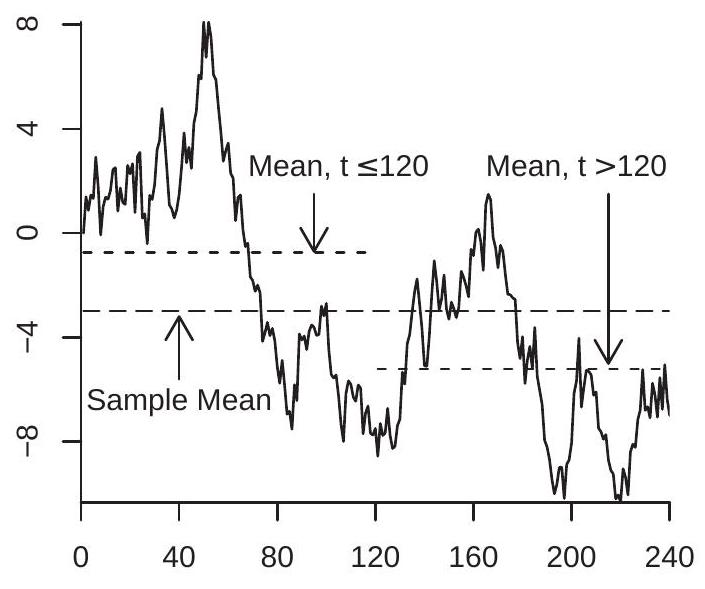
\includegraphics[max width=\textwidth]{2022_10_23_e99fc7c58db661c6f219g-08}

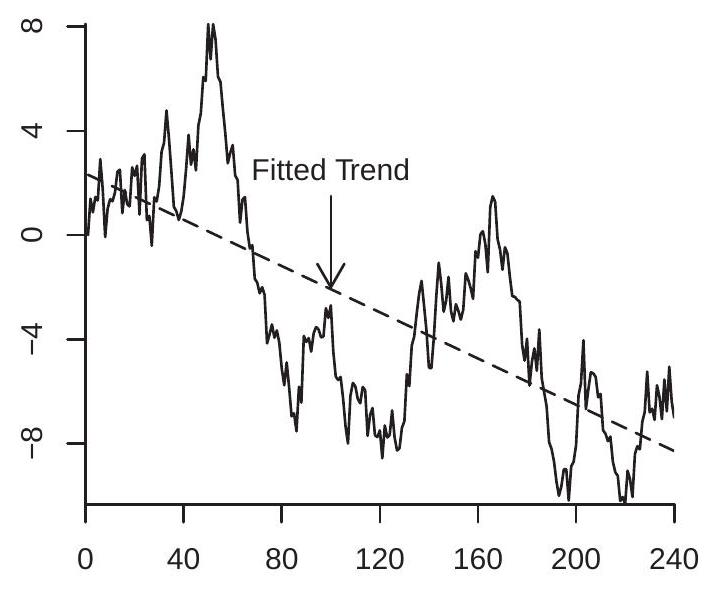
\includegraphics[max width=\textwidth]{2022_10_23_e99fc7c58db661c6f219g-08(1)}

(a) Fitted Means

(b) Fitted Trend

Figure 16.1: Random Walk with Fitted Mean, Sub-Sample Means, and Trend

To illustrate, Figure 16.1(a) displays a simulated random walk with $n=240$ observations. Also plotted is the sample mean $\bar{Y}_{n}=-2.98$, along with the sub-sample means $\bar{Y}_{1 n}=-0.75$ and $\bar{Y}_{2 n}=-5.21$. As predicted, the mean and sub-sample means are large, variable, and uninformative regarding the population mean.

Now consider a linear regression of $Y_{t}$ on a linear time trend. The model for estimation is
$$
Y_{t}=\beta_{0}+\beta_{1} t+e_{t}=X_{t}^{\prime} \beta+e_{t}
$$
where $X_{t}=(1, t)^{\prime}$. Again for simplicity assume that $Y_{0}=0$. Take the least squares estimator $\widehat{\beta}$. Theorem $14.36$ shows that
$$
\begin{gathered}
\frac{1}{n^{2}} \sum_{t=1}^{n} t \rightarrow \int_{0}^{1} r d r=\frac{1}{2} \\
\frac{1}{n^{3}} \sum_{t=1}^{n} t^{2} \rightarrow \int_{0}^{1} r^{2} d r=\frac{1}{3} .
\end{gathered}
$$
Define $D_{n}=\left[\begin{array}{ll}1 & 0 \\ 0 & n\end{array}\right]$. We calculate that
$$
D_{n}^{-1} \frac{1}{n} \sum_{t=1}^{n} X_{t} X_{t}^{\prime} D_{n}^{-1}=\left[\begin{array}{cc}
\frac{1}{n} \sum_{t=1}^{n} 1 & \frac{1}{n^{2}} \sum_{t=1}^{n} t \\
\frac{1}{n^{2}} \sum_{t=1}^{n} t & \frac{1}{n^{3}} \sum_{t=1}^{n} t^{2}
\end{array}\right] \rightarrow\left[\begin{array}{cc}
1 & \int_{0}^{1} r d r \\
\int_{0}^{1} r d r & \int_{0}^{1} r^{2} d r
\end{array}\right]=\int_{0}^{1} X(r) X(r)^{\prime} d r
$$
where $X(r)=(1, r)$.

An application of the continuous mapping theorem with Theorem $16.1$ yields
$$
D_{n}^{-1} \frac{1}{n^{3 / 2}} \sum_{t=1}^{n} X_{t} Y_{t}=\int_{0}^{1} X(r) Z_{n}(r) d r \underset{d}{\longrightarrow} \int_{0}^{1} X(r) B(r) d r .
$$
Together we obtain
$$
\begin{aligned}
D_{n} n^{-1 / 2} \widehat{\beta} &=D_{n} n^{-1 / 2}\left(\sum_{t=1}^{n} X_{t} X_{t}^{\prime}\right)^{-1}\left(\sum_{t=1}^{n} X_{t} Y_{t}\right) \\
&=\left(D_{n}^{-1} \frac{1}{n} \sum_{t=1}^{n} X_{t} X_{t}^{\prime} D_{n}^{-1}\right)^{-1}\left(D_{n}^{-1} \frac{1}{n^{3 / 2}} \sum_{t=1}^{n} X_{t} Y_{t}\right) \\
& \underset{d}{\longrightarrow}\left(\int_{0}^{1} X(r) X(r)^{\prime} d r\right)^{-1}\left(\int_{0}^{1} X(r) B(r) d r\right) .
\end{aligned}
$$
This shows that the estimator $\widehat{\beta}$ has an asymptotic distribution which is a transformation of the Brownian motion $B(r)$. For compactness we often write the final expression as $\left(\int_{0}^{1} X X^{\prime}\right)^{-1}\left(\int_{0}^{1} X B\right)$.

To illustrate, Figure 16.1(b) displays the random walk from panel (a) along with a fitted trend line. The fitted trend appears large and substantial. However it is purely random, a feature only of this specific realization, is uninformative about the underlying parameters, and is dangerously misleading for prediction.

\subsection{Demeaning and Detrending}
A common preliminary step in time series analysis is demeaning (subtracting off a mean) and detrending (subtracting off a linear trend). With stationary processes this does not affect asymptotic inference. In contrast, an important property of unit root processes is that their behavior is altered by these transformations.

Take demeaning. The demeaned version of $Y_{t}$ is $Y_{t}^{*}=Y_{t}-\bar{Y}_{n}$. An important observation is that $Y_{t}^{*}$ is invariant to the initial condition $Y_{0}$, so without loss of generality we simply assume $Y_{0}=0$.

The normalized process is
$$
Z_{n}^{*}(r)=\frac{1}{\sqrt{n}} Y_{\lfloor n r\rfloor}-\frac{1}{\sqrt{n}} \bar{Y}_{n}=Z_{n}(r)-Z_{n}(1) \underset{d}{\longrightarrow} B(r)-\int_{0}^{1} B \stackrel{\text { def }}{=} B^{*}(r) .
$$
$B^{*}(r)$ is demeaned Brownian motion. It has the property that $\int_{0}^{1} B^{*}(r) d r=0$.

Take linear detrending. Based on least squares estimation of a linear trend the detrended series is $Y_{t}^{* *}=Y_{t}-X_{t}^{\prime} \widehat{\beta}$ where $X_{t}=(1, t)^{\prime}$. Like the demeaned series the detrended series is invariant to $Y_{0}$. The associated normalized process is
$$
\begin{aligned}
& Z_{n}^{* *}(r)=\frac{1}{\sqrt{n}} Y_{\lfloor n r\rfloor}-\frac{1}{\sqrt{n}} X_{\lfloor n r\rfloor}^{\prime} \widehat{\beta} \\
& =Z_{n}(r)-X(\lfloor n r\rfloor / n)^{\prime} D_{n} \frac{1}{\sqrt{n}} \widehat{\beta} \\
& \underset{d}{\longrightarrow} B(r)-X(r)^{\prime}\left(\int_{0}^{1} X X^{\prime}\right)^{-1}\left(\int_{0}^{1} X B\right) \stackrel{\text { def }}{=} B^{* *}(r) .
\end{aligned}
$$
$B^{* *}(r)$ is the continuous-time residual of the Brownian motion $B(r)$ projected orthogonal to $X(r)=$ $(1, r)^{\prime}$. We call $B^{* *}(r)$ detrended Brownian motion.

There is another method of detrending through first differencing. Suppose that $Y_{t}=\beta_{0}+\beta_{1} t+Z_{t}$. The first difference is $\Delta Y_{t}=\beta_{1}+\Delta Z_{t}$. An estimator of $\beta_{1}$ is the sample mean of $\Delta Y_{t}$ :
$$
\overline{\Delta Y}_{n}=\frac{1}{n} \sum_{t=1}^{n} \Delta Y_{t}=\frac{Y_{n}-Y_{0}}{n} .
$$
The normalization $Z_{0}=0$ implies $Y_{0}=\beta_{0}$ so an estimator of $\beta_{0}$ is $Y_{0}$. The detrended version of $Y_{t}$ is $\widetilde{Y}_{t}=Y_{t}-Y_{0}-(t / n)\left(Y_{n}-Y_{0}\right)$. The associated normalized process is
$$
\widetilde{Z}_{n}(r)=Z_{n}(r)-\frac{\lfloor n r\rfloor}{n} Z_{n}(1) \underset{d}{\longrightarrow} B(r)-r B(1) \stackrel{\text { def }}{=} V(r) .
$$
$V(r)$ is called a Brownian Bridge or a tied-down Brownian motion. It has the property that $V(0)=V(1)=$ 0 . It is also a detrended version of $B(r)$ but is distinct from the linearly detrended version $B^{*}(r)$.

We summarize the findings in the following theorem.

Theorem 16.5 Under the conditions of either Theorem $16.3$ or Theorem 16.4, then as $n \rightarrow \infty$

\begin{enumerate}
  \item $Z_{n}^{*}(r) \underset{d}{\longrightarrow} B^{*}(r)$

  \item $Z_{n}^{* *}(r) \underset{d}{\longrightarrow} B^{* *}(r)$

  \item $\widetilde{Z}_{n}(r) \underset{d}{\longrightarrow} V(r)$

\end{enumerate}
To illustrate, Figure $16.2$ displays two detrended versions of the series from Figure 16.1. Panel (a) shows the linear detrended series $Y_{t}^{*}$. Panel (b) shows the first-difference detrended series $\widetilde{Y}_{t}$. They are visually similar to one another and to Figure $16.1$ except that the strong linear trend has been removed.

\subsection{Stochastic Integrals}
The distribution of the least squares estimator in the regression model $Y_{t}=X_{t}^{\prime} \beta+e_{t}$ requires the distribution of the sample moments $n^{-1} \sum_{t=1}^{n-1} X_{t} e_{t+1}$. When $X_{t}$ is non-stationary the limit distribution is non-standard and equals a stochastic integral.

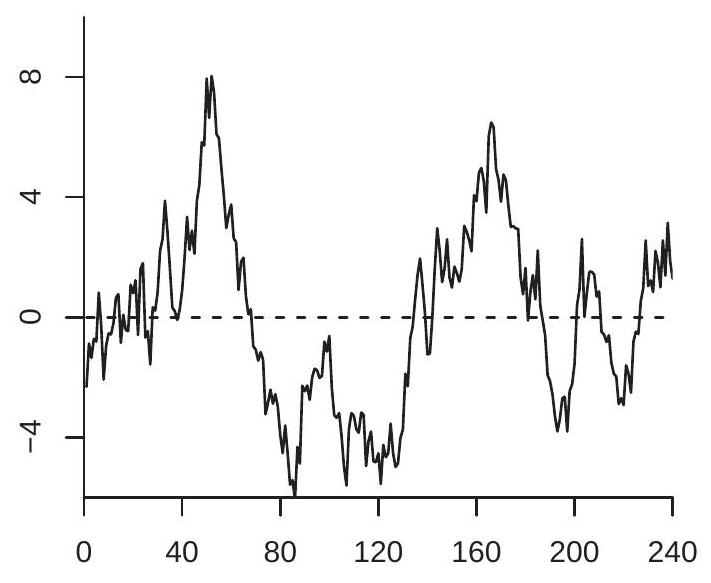
\includegraphics[max width=\textwidth]{2022_10_23_e99fc7c58db661c6f219g-11}

(a) Linearly Detrended Series

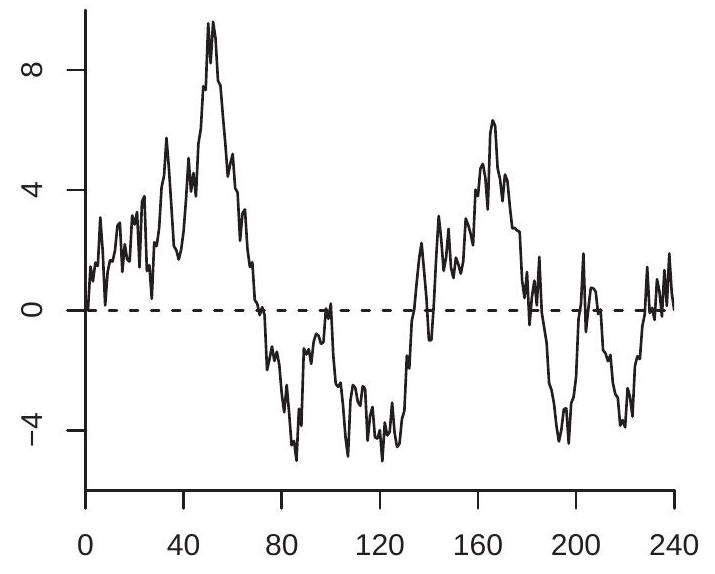
\includegraphics[max width=\textwidth]{2022_10_23_e99fc7c58db661c6f219g-11(1)}

(b) First Difference Detrended Series

Figure 16.2: Detrended Random Walk

It may help to recall the definition of the Riemann-Stieltijes integral. Over the region $[0,1]$ the integral of $g(x)$ with respect to $f(x)$ is
$$
\int_{0}^{1} g(x) d f(x)=\lim _{N \rightarrow \infty} \sum_{i=0}^{N-1} g\left(\frac{i}{N}\right)\left(f\left(\frac{i+1}{N}\right)-f\left(\frac{i}{N}\right)\right) .
$$
A stochastic integral is the case where the function $f$ is random and is defined as a probability limit.

Definition 16.4 The stochastic integral of vector-valued $X(r)$ with respect to vector-valued $Z(r)$ over $[0,1]$ is
$$
\int_{0}^{1} X d Z^{\prime}=\int_{0}^{1} X(r) d Z(r)^{\prime}=\underset{N \rightarrow \infty}{\operatorname{plim}} \sum_{i=0}^{N-1} X\left(\frac{i}{N}\right)\left(Z\left(\frac{i+1}{N}\right)-Z\left(\frac{i}{N}\right)\right)^{\prime} .
$$
Now consider the following setting. Let $\left(X_{t}, e_{t}\right)$ be vector-valued sequences where $e_{t}$ is a MDS with finite covariance and $X_{t}$ is non-stationary. Assume that for some scaling sequence $D_{n}$ the scaled process $X_{n}(r)=D_{n}^{-1} X_{\lfloor n r\rfloor}$ satisfies $X_{n}(r) \underset{d}{\longrightarrow} X(r)$ for some deterministic or stochastic process $X(r)$. Examples of $X_{t}$ sequences include the partial sum process constructed from $e_{t}$ or another shock, a detrended version of a partial sum process, or a deterministic trend proceses. We desire the asymptotic distribution of $\sum_{t=1}^{n-1} X_{t} e_{t+1}^{\prime}$. Define the partial sum process for $e_{t}$ as $S_{n}(r)=n^{-1 / 2} \sum_{t=1}^{\lfloor n r\rfloor} e_{t}$. From Theorem 16.1, $S_{n} \underset{d}{\longrightarrow}$ $B$. We calculate that
$$
\frac{1}{\sqrt{n}} D_{n}^{-1} \sum_{t=0}^{n-1} X_{t} e_{t+1}^{\prime}=\sum_{t=0}^{n-1} X_{n}\left(\frac{t}{n}\right)\left(S_{n}\left(\frac{t+1}{n}\right)-S_{n}\left(\frac{t}{n}\right)\right)^{\prime}=\int_{0}^{1} X_{n} d S_{n}^{\prime} .
$$
The equalities hold because $S_{n}(r)$ and $X_{n}(r)$ are step functions with jumps at $r=t / n$. Since $X_{n}(r)$ and $S_{n}(r)$ converge to $X(r)$ and $B(r)$, by analogy we expect $\int_{0}^{1} X_{n} d S_{n}$ to converge to $\int_{0}^{1} X d B$. This is true, but rather tricky to show since the stochastic integral is not a continuous function of $B(r)$. A general statement of the conditions has been provided by Kurtz and Protter (1991, Theorem 2.2). The following is a simplification of their result.

Theorem 16.6 If $\left(e_{t}, \mathscr{F}_{t}\right)$ is a martingale difference sequence, $\mathbb{E}\left[e_{t} e_{t}^{\prime}\right]=\Sigma<\infty$, $X_{t} \in \mathscr{F}_{t}$, and $\left(X_{n}(r), S_{n}(r)\right) \underset{d}{\longrightarrow}(X(r), B(r))$ then
$$
\int_{0}^{1} X_{n} d S_{n}^{\prime}=\frac{1}{\sqrt{n}} D_{n}^{-1} \sum_{t=1}^{n-1} X_{t} e_{t+1} \underset{d}{\longrightarrow} \int_{0}^{1} X d B^{\prime}
$$
where $B(r)$ is a Brownian motion with covariance matrix $\Sigma$.

The basic application of Theorem $16.6$ is to the case $X_{n}(r)=S_{n}(r)$. Thus if $S_{t}=\sum_{i=1}^{t} e_{t}$ and $e_{t}$ is a MDS with covariance matrix $\Sigma$ then
$$
\frac{1}{n} \sum_{t=1}^{n-1} S_{t} e_{t+1}^{\prime} \underset{d}{\longrightarrow} \int_{0}^{1} B d B^{\prime} .
$$
We can extend this result to the case of serially correlated errors.

Theorem 16.7 If $Z_{t}$ satisfies the conditions of Theorem $16.4$ and $S_{t}=\sum_{i=1}^{t} Z_{t}$ then
$$
\frac{1}{n} \sum_{t=1}^{n-1} S_{t} Z_{t+1}^{\prime} \underset{d}{\longrightarrow} \int_{0}^{1} B d B^{\prime}+\Lambda
$$
where $B(r)$ is a Brownian motion with covariance matrix $\Omega=\Sigma+\Lambda+\Lambda^{\prime}, \Sigma=$ $\mathbb{E}\left[Z_{t} Z_{t}^{\prime}\right]$, and $\Lambda=\sum_{j=1}^{\infty} \mathbb{E}\left[Z_{t-j} Z_{t}^{\prime}\right]$

The proof is presented in Section $16.22$.

\subsection{Estimation of an $\mathbf{A R}(1)$}
Consider least squares estimation of the AR(1) parameter $\alpha$ in the model $Y_{t}=\alpha Y_{t-1}+e_{t}$. The centered estimator is $\widehat{\alpha}-\alpha=\left(\sum_{t=1}^{n-1} Y_{t}^{2}\right)^{-1}\left(\sum_{t=1}^{n-1} Y_{t} e_{t+1}\right)$. We use the scaling
$$
n(\widehat{\alpha}-\alpha)=\frac{\frac{1}{n} \sum_{t=1}^{n-1} Y_{t} e_{t+1}}{\frac{1}{n^{2}} \sum_{t=1}^{n-1} Y_{t}^{2}} .
$$
We examine the denominator and numerator separately under the assumption $\alpha=1$. Similarly to our analysis of the sample mean the denominator can be written as an integral. Thus
$$
\frac{1}{n^{2}} \sum_{t=1}^{n-1} Y_{t}^{2}=\frac{1}{n} \sum_{t=1}^{n-1}\left(\frac{1}{n^{1 / 2}} Y_{t}\right)^{2}=\int_{0}^{1} Z_{n}(r)^{2} d r \underset{d}{\longrightarrow} \int_{0}^{1} B(r)^{2} d r=\sigma^{2} \int_{0}^{1} W(r)^{2} d r
$$
The convergence is by the continuous mapping theorem ${ }^{4}$. The final equality recognizes that if $B(r)$ has variance $\sigma^{2}$ then $B(r)^{2}=\sigma^{2} W(r)^{2}$ where $W(r)$ is standard Brownian motion. For conciseness we often write the final integral as $\int_{0}^{1} W^{2}$.

For the numerator we appeal to Theorem 16.6.
$$
\frac{1}{n} \sum_{t=1}^{n-1} Y_{t} e_{t+1}=\int_{0}^{1} Z_{n} d S_{n} \underset{d}{\longrightarrow} \int_{0}^{1} B d B=\sigma^{2} \int_{0}^{1} W d W .
$$
This limiting stochastic integral is quite famous. It is known as Itô's integral.

Theorem 16.8 Itô's Integral $\int_{0}^{1} W d W=\frac{1}{2}\left(W(1)^{2}-1\right)$

If you are not surprised by Itô's integral take another look. The derivative of $\frac{1}{2} W(r)^{2}$ is $W(r) d W(r)$. Thus by standard calculus and $W(0)=0$ you might expect $\int_{0}^{1} W d W=\frac{1}{2} W(1)^{2}$. The presence of the extra term $-1 / 2$ is surprising. This arises because $W(r)$ has unbounded variation.

The random variable $W(1)^{2}$ is $\chi_{1}^{2}$ which has expectation 1 . Therefore the random variable $\int_{0}^{1} W d W$ is mean zero but skewed.

The proof of Theorem $16.8$ is presented in Section $16.22$.

Returning to the least squares estimation problem we have shown that when $\alpha=1$
$$
n(\widehat{\alpha}-1) \underset{d}{\longrightarrow} \frac{\frac{\sigma^{2}}{2}\left(W(1)^{2}-1\right)}{\sigma^{2} \int_{0}^{1} W^{2}}=\frac{\int_{0}^{1} W d W}{\int_{0}^{1} W^{2}} .
$$
Theorem 16.9 Dickey-Fuller Coefficient Distribution If $Y_{t}=\alpha Y_{t-1}+e_{t}$ with $\alpha=1$, and $\left(e_{t}, \mathscr{F}_{t}\right)$ is a strictly stationary and ergodic martingale difference sequence with a finite variance, then
$$
n(\widehat{\alpha}-1) \underset{d}{\longrightarrow} \frac{\int_{0}^{1} W d W}{\int_{0}^{1} W^{2}} .
$$
The limit distribution in Theorem $16.9$ is known as the Dickey-Fuller Distribution due to the work of Wayne Fuller and David Dickey. Theorem 16.9 shows that the least squares estimator is consistent for $\alpha=1$ and converges at the "super-consistent" rate $O_{p}\left(n^{-1}\right)$. The limit distribution is non-standard and is written as a function of the Brownian motion $W(r)$. There is not a closed-form expression for the distribution or density of the statistic. Most commonly it is calculated by simulation.

${ }^{4}$ The function $g(f)=\int_{0}^{1} f(x)^{2} d x$ is continuous with respect to the uniform metric. The density of the Dickey-Fuller coefficient distribution is displayed ${ }^{5}$ in Figure $16.3$ (a) with the label "No Intercept". You can see that the density is high skewed with a long left tail. You can see that most of the probability mass of the distribution is over the negative region. This has the implication that the density has a negative mean and median. Hence the asymptotic distribution of the least squares estimator is biased negatively. This has the practical implication that when $\alpha=1$ the least squares estimator is biased away from one.

We can also examine the limit distribution of the t-ratio. Let $\widehat{e}_{t}=Y_{t}-\widehat{\alpha} Y_{t-1}$ be the least squares residual, $\widehat{\sigma}^{2}=n^{-1} \sum \widehat{e}_{t}^{2}$ the least squares variance estimator, and $s(\widehat{\alpha})=\widehat{\sigma} / \sqrt{\sum Y_{t}^{2}}$ the classical standard error for $\widehat{\alpha}$. The t-ratio for $\alpha$ is $T=(\widehat{\alpha}-1) / s(\widehat{\alpha})$.

Theorem 16.10 Dickey-Fuller T Distribution Under the assumptions of Theorem $16.9$
$$
T=\frac{\widehat{\alpha}-1}{s(\widehat{\alpha})} \underset{d}{\longrightarrow} \frac{\int_{0}^{1} W d W}{\left(\int_{0}^{1} W^{2}\right)^{1 / 2}} .
$$
The limit distribution in Theorem $16.10$ is known as the Dickey-Fuller T distribution. Theorem $16.10$ shows that the classical t-ratio converges to a non-standard asymptotic distribution. There is no closedform expression for the distribution or density so it is typically calculated using simulation techniques. The proof is presented in Section $16.22$.

The density of the Dickey-Fuller T distribution is displayed in Figure 16.3(b) with the label "No Intercept". You can see that the density is skewed but much less so than the coefficient distribution. The distribution appears to be a "fatter" version of the conventional student t distribution. An implication is that conventional inference (confidence intervals and tests) will be inaccurate. We discuss testing in Section $16.13$.

\subsection{AR(1) Estimation with an Intercept}
Suppose that $Y_{t}$ is a random walk and we estimate an AR(1) model with an intercept. The estimated model is $Y_{t}=\mu+\alpha Y_{t-1}+e_{t}$. By the Frisch-Waugh-Lovell Theorem (Theorem 3.5) the least squares estimator $\widehat{\alpha}$ of $\alpha$ can be written as the simple regression using the demeaned series $Y_{t}^{*}$. That is, the normalized estimator is
$$
n(\widehat{\alpha}-1)=\frac{\frac{1}{n} \sum_{t=1}^{n-1} Y_{t}^{*} e_{t+1}}{\frac{1}{n^{2}} \sum_{t=1}^{n-1} Y_{t}^{* 2}}
$$
where $Y_{t}^{*}=Y_{t}-\bar{Y}$ with $\bar{Y}=\frac{1}{n} \sum_{t=1}^{n-1} Y_{t}$. By Theorems 16.5.1 and $16.6$ the calculations from the previous section show that
$$
n(\widehat{\alpha}-1) \underset{d}{\longrightarrow} \frac{\int_{0}^{1} W^{*} d W}{\int_{0}^{1} W^{* 2}} .
$$
${ }^{5}$ The densities in Figure $16.3$ were estimated from one million simulation draws of the finite sample distribution for a sample size $n=10,000$. The densities were estimated using nonparametric kernel methods (see Chapter 17 of Introduction to Econometrics).

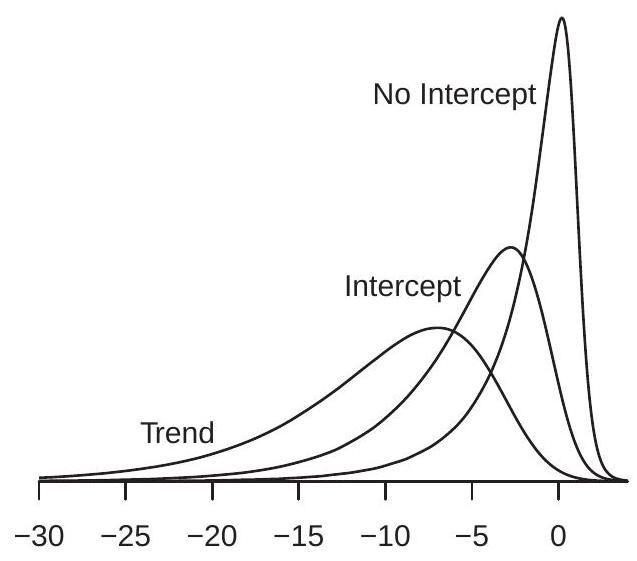
\includegraphics[max width=\textwidth]{2022_10_23_e99fc7c58db661c6f219g-15}

(a) Dickey-Fuller Coefficient Density

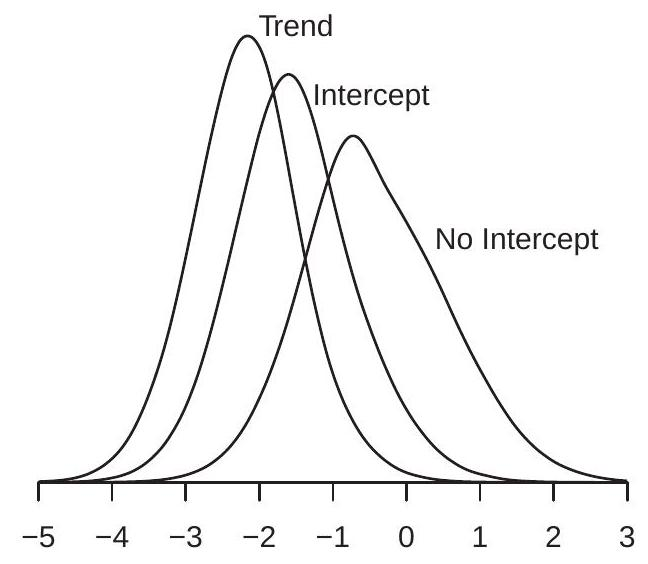
\includegraphics[max width=\textwidth]{2022_10_23_e99fc7c58db661c6f219g-15(1)}

(b) Dickey-Fuller T Density

Figure 16.3: Unit Root Distributions

This is similar to the distribution in Theorem 16.9. This is known as the Dickey-Fuller coefficient distribution for the case of an included intercept.

Similarly if we estimate an AR(1) model with an intercept and trend the estimated model is $Y_{t}=$ $\mu+\beta t+\alpha Y_{t-1}+e_{t}$. By the Frisch-Waugh-Lovell Theorem this is equivalent to regression on the detrended series $Y_{t}^{* *}$. Applying Theorems $16.5 .2$ and 16.6, we find
$$
n(\widehat{\alpha}-1) \underset{d}{\longrightarrow} \frac{\int_{0}^{1} W^{* *} d W}{\int_{0}^{1} W^{* * 2}} .
$$
This is known as the Dickey-Fuller coefficient distribution for the case of an included intercept and linear trend.

Similar results arise for the t-ratios. We summarize the results in the following theorem. Theorem 16.11 Under the assumptions of Theorem 16.9, for the case of an estimated AR(1) with an intercept
$$
\begin{gathered}
n(\widehat{\alpha}-1) \underset{d}{\longrightarrow} \frac{\int_{0}^{1} W^{*} d W}{\int_{0}^{1} W^{* 2}} \\
T \underset{d}{\longrightarrow} \frac{\int_{0}^{1} W^{*} d W}{\left(\int_{0}^{1} W^{* 2}\right)^{1 / 2}} .
\end{gathered}
$$
For the case of an estimated AR(1) with an intercept and linear time trend
$$
\begin{gathered}
n(\widehat{\alpha}-1) \underset{d}{\longrightarrow} \frac{\int_{0}^{1} W^{* *} d W}{\int_{0}^{1} W^{* * 2}} \\
T \underset{d}{\longrightarrow} \frac{\int_{0}^{1} W^{* *} d W}{\left(\int_{0}^{1} W^{* * 2}\right)^{1 / 2}} .
\end{gathered}
$$
The densities of the Dickey-Fuller coefficient distributions are displayed in Figure 16.3(a), labeled as "Intercept" for the case with an included intercept, and "Trend" for the case with an intercept and linear time trend. The densities are considerably affected by the inclusion of the intercept or intercept and trend. The effect is twofold: (1) the distributions shift substantially to the left; and (2) the distributions substantially widen. Examining the "trend" version we can see that there is very little probability mass above zero. This means that the asymptotic distribution is not only biased downward, the realization is nearly always negative. This has the practical implication that the least squares estimator is almost certainly less than the true coefficient value. This is a strong form of bias.

The densities of the Dickey-Fuller T distributions are displayed in Figure 16.3(b). The effect of detrending on the $\mathrm{T}$ distributions is quite different from the effect on the coefficient distirbutions. Here we see that the primary effect is a location shift with only a mild impact on dispersion. The strong location shift is a bias in the asymptotic $\mathrm{T}$ distribution, implying that conventional inferences will be incorrect.

\subsection{Sample Covariances of Integrated and Stationary Processes}
Let $\left(X_{t}, u_{t}\right)$ be a sequence where $X_{t}$ is non-stationary and $u_{t}$ is mean zero and strictly stationary. Assume that for some scaling sequence $D_{n}$ the scaled process $X_{n}(r)=D_{n}^{-1} X_{\lfloor n r\rfloor}$ satisfies $X_{n}(r) \underset{d}{\longrightarrow} X(r)$ where $X(r)$ is continuous with probability one. Consider the scaled sample covariance
$$
C_{n}=\frac{1}{n} D_{n}^{-1} \sum_{t=1}^{n} X_{t} u_{t} .
$$
Theorem 16.12 Assume that $X_{n}(r)=D_{n}^{-1} X_{\lfloor n r\rfloor} \underset{d}{\longrightarrow} X(r)$ where $X(r)$ is almost surely continuous. Assume $u_{t}$ is mean zero, strictly stationary, ergodic, and $\mathbb{E}\left|u_{t}\right|<\infty$. Then $C_{n} \underset{p}{\longrightarrow} 0$ as $n \rightarrow \infty$. The proof is presented in Section $16.22$.

\subsection{AR(p) Models with a Unit Root}
Assume that $Y_{t}$ satisfies $a(\mathrm{~L}) \Delta Y_{t}=e_{t}$ where $a(z)$ is a $p-1$ order invertible lag polynomial and $e_{t}$ is a stationary MDS with finite variance $\sigma^{2}$. Then $Y_{t}$ can be written as the AR(p) process
$$
Y_{t}=a_{1} Y_{t-1}+\cdots+a_{p} Y_{t-p}+e_{t}
$$
where the coefficients satisfy $a_{1}+\cdots+a_{p}=1$. Let $\widehat{a}$ be the least squares estimator of $a=\left(a_{1}, \ldots, a_{p}\right)$. We now describe its sampling distribution.

Let $B$ be the $p \times p$ matrix which transforms $\left(Y_{t-1}, \ldots, Y_{t-p}\right)$ to $\left(Y_{t-1}, \Delta Y_{t-1}, \ldots, \Delta Y_{t-p+1}\right)$, for example when $p=3$ then $B=\left[\begin{array}{ccc}1 & 0 & 0 \\ 1 & -1 & 0 \\ 0 & 1 & -1\end{array}\right]$. Make the partition $B^{-1 \prime} a=(\rho, \beta)$ where $\rho \in \mathbb{R}$ and $\beta \in \mathbb{R}^{p-1}$. Then the $\mathrm{AR}(\mathrm{p})$ model can be written as
$$
Y_{t}=\rho Y_{t-1}+\beta^{\prime} X_{t-1}+e_{t}
$$
where $X_{t-1}=\left(\Delta Y_{t-1}, \ldots, \Delta Y_{t-p+1}\right)$. The leading coefficient is $\rho=a_{1}+\cdots+a_{p}=1$. This transformation separates the regressors into the unit root component $Y_{t-1}$ and the stationary component $X_{t-1}$.

Consider the least squares estimators $(\widehat{\rho}, \widehat{\beta})$. They can be written under the assumption of a unit root as
$$
\left(\begin{array}{c}
n(\widehat{\rho}-1) \\
\sqrt{n}(\widehat{\beta}-\beta)
\end{array}\right)=\left(\begin{array}{cc}
\frac{1}{n^{2}} \sum_{t=1+p}^{n} Y_{t-1}^{2} & \frac{1}{n^{3 / 2}} \sum_{t=1+p}^{n} Y_{t-1} X_{t-1}^{\prime} \\
\frac{1}{n^{3 / 2}} \sum_{t=1+p}^{n} X_{t-1} Y_{t-1} & \frac{1}{n} \sum_{t=1+p}^{n} X_{t-1} X_{t-1}^{\prime}
\end{array}\right)^{-1}\left(\begin{array}{c}
\frac{1}{n} \sum_{t=1+p}^{n} Y_{t-1} e_{t} \\
\frac{1}{\sqrt{n}} \sum_{t=1+p}^{n} X_{t-1} e_{t}
\end{array}\right) .
$$
Theorems $16.4$ and the CMT show that
$$
\frac{1}{n^{2}} \sum_{t=1+p}^{n} Y_{t-1}^{2} \underset{d}{\rightarrow} \omega^{2} \int_{0}^{1} W^{2}
$$
where $\omega^{2}$ is the long-run variance of $\Delta Y_{t}$ which equals $\omega^{2}=\sigma^{2} / a(1)^{2}>0$.

Theorem $16.12$ shows that
$$
\frac{1}{n^{3 / 2}} \sum_{t=1+p}^{n} X_{t-1} Y_{t-1} \underset{p}{\longrightarrow} 0 .
$$
Theorems $16.4$ and $16.6$ show that
$$
\frac{1}{n} \sum_{t=1+p}^{n} Y_{t-1} e_{t} \underset{d}{\longrightarrow} \omega \sigma \int_{0}^{1} W d W .
$$
The WLLN and the CLT for stationary processes show that
$$
\begin{aligned}
&\frac{1}{n} \sum_{t=1+p}^{n} X_{t-1} X_{t-1}^{\prime} \rightarrow \boldsymbol{Q} \\
&\frac{1}{\sqrt{n}} \sum_{t=1+p}^{n} X_{t-1} e_{t} \underset{d}{\longrightarrow} \mathrm{N}(0, \Omega)
\end{aligned}
$$
where $\boldsymbol{Q}=\mathbb{E}\left[X_{t-1} X_{t-1}^{\prime}\right]$ and $\Omega=\mathbb{E}\left[X_{t-1} X_{t-1}^{\prime} e_{t}^{2}\right]$. Together we have established the following. Theorem 16.13 Assume that $Y_{t}$ satisfies $a(\mathrm{~L}) \Delta Y_{t}=e_{t}$ where $a(z)$ is a $p-1$ order invertible lag polynomial and $\left(e_{t}, \Im_{t}\right)$ is a stationary MDS with finite variance $\sigma^{2}$. Then
$$
\left(\begin{array}{c}
n(\widehat{\rho}-1) \\
\sqrt{n}(\widehat{\beta}-\beta)
\end{array}\right) \rightarrow\left(\begin{array}{c}
a(1) \frac{\int_{0}^{1} W d W}{\int_{0}^{1} W^{2}} \\
\mathrm{~N}(0, V)
\end{array}\right)
$$
where $V=\boldsymbol{Q}^{-1} \Omega \boldsymbol{Q}^{-1}$.

This theorem provides an asymptotic distribution theory for the least squares estimators. The estimator $(\widehat{a}, \widehat{\beta})$ is consistent, the coefficient $\widehat{\beta}$ on the stationary variables is asymptotically normal, and the coefficient $\widehat{a}$ on the unit root component has a scaled Dickey-Fuller distribution.

The estimator of the representation (16.6) is the linear transformation $B^{\prime}\left(\widehat{\rho}, \widehat{\beta}^{\prime}\right)^{\prime}$, and therefore its asymptotic distribution is the transformation $B^{\prime}$ of (16.8). Since the unit root component converges at a faster $O_{p}\left(n^{-1}\right)$ rate than the stationary component it drops out of the asymptotic distribution. We obtain
$$
\sqrt{n}(\widehat{a}-a) \underset{d}{\longrightarrow} \mathrm{N}\left(0, \boldsymbol{G} V \boldsymbol{G}^{\prime}\right)
$$
where, in the $p=3$ case
$$
\boldsymbol{G}=\left[\begin{array}{cc}
1 & 0 \\
-1 & 1 \\
0 & -1
\end{array}\right] \text {. }
$$
The asymptotic covariance matrix $\boldsymbol{G} V \boldsymbol{G}^{\prime}$ is deficient with rank $p-1$. Hence this is only a partial characterization of the asymptotic distribution; equation (16.8) is a complete first-order characterization. The implication of (16.9) is that individual coefficient estimators and standard errors of (16.6) have conventional asymptotic interpretations. This extends to conventional hypothesis tests which do not include the sum of the coefficients. For most purposes (except testing the unit root hypothesis) this means that asymptotic inference on the coefficients of (16.6) can be based on the conventional normal approximation and can ignore the possible presence of unit roots.

\subsection{Testing for a Unit Root}
The asymptotic properties of the time series process change discontinuously at the unit root $\rho=$ $a_{1}+\cdots+a_{p}=1$. It is therefore of standard interest to test the hypothesis of a unit root. We typically express this as the test of $\mathbb{H}_{0}: \rho=1$ against $\mathbb{H}_{1}: \rho<1$. We typically view the test as one-sided as we are interested in the alternative hypothesis that the series is stationary (not that it is explosive).

The test for $\mathbb{H}_{0} \mathrm{vs} . \mathbb{H}_{1}$ is the t-statistic for $a_{1}+\cdots+a_{p}=1$ in the AR(p) model (16.6). This is identical to the t-statistic for $\rho=1$ in reparameterized form (16.7). Since the latter is a simple t-ratio this is the most convenient implementation. It is typically called the Augmented Dickey-Fuller statistic. It equals
$$
\mathrm{ADF}=\frac{\widehat{\rho}-1}{s(\widehat{\rho})}
$$
where $s(\widehat{\rho})$ is a standard error for $\widehat{\rho}$. This t-ratio is typically calculated using a classical (homoskedastic) standard error, perhaps for historical reasons, and perhaps because the asymptotic distribution of ADF is invariant to conditional heteroskedasticity. The statistic is called the ADF statistic when the estimated model is an $\operatorname{AR}(\mathrm{p})$ model with $p>1$; it is typically called the Dickey-Fuller statistic if the estimated model is an $\operatorname{AR}(1)$.

The asymptotic distribution of ADF depends on the fitted deterministic components. The test statistic is most typically calculated in a model with a fitted intercept or a fitted intercept and time trend, though the theory is also presented for the case with no fitted intercept, and extends to any polynomial order trend.

Theorem 16.14 Assume that $Y_{t}$ satisfies $a(\mathrm{~L}) \Delta Y_{t}=e_{t}$ where $a(z)$ is a $p-1$ order invertible lag polynomial and $\left(e_{t}, \Im_{t}\right)$ is a stationary MDS with finite variance $\sigma^{2}$. Then
$$
\mathrm{ADF} \underset{d}{\longrightarrow} \frac{\int_{0}^{1} U d W}{\left(\int_{0}^{1} U^{2}\right)^{1 / 2}} \stackrel{\text { def }}{=} \xi
$$
where $W$ is Brownian motion. The process $U$ depends on the fitted deterministic components:

\begin{enumerate}
  \item Case 1: No intercept or trend. $U(r)=W(r)$.

  \item Case 2: Fitted intercept (demeaned data). $U(r)=W(r)-r \int_{0}^{1} W$.

  \item Case 3: Fitted intercept and trend (detrended data). $U(r)=W(r)-$ $X(r)^{\prime}\left(\int_{0}^{1} X X^{\prime}\right)^{-1}\left(\int_{0}^{1} X W\right)$ where $X(r)=(1, r)^{\prime}$.

\end{enumerate}
Let $Z_{\alpha}$ satisfy $\mathbb{P}\left[\xi \leq Z_{\alpha}\right]=\alpha$. The test "Reject $\mathbb{H}_{0}$ if $\mathrm{ADF}<Z_{\alpha}$ " has asymptotic size $\alpha$

Asymptotic critical values are displayed in the first three columns of Table 16.1. The ADF is a onesided hypothesis test so rejections occur when the test statistic is less than (more negative than) the critical value. For example, the $5 \%$ critical value for the case of a fitted intercept is $-2.86$. This means that if the ADF t-ratio is more negative than $-2.86$ (for example $\mathrm{ADF}=-3.0$ ) then the test rejects the hypothesis of no unit root. But if the ADF t-ratio is greater than $-2.86$ (for example ADF $=-2.0$ ) then the the test does not reject the hypothesis of a unit root.

In most applications an ADF test is implemented with at least a fitted intercept (the second column in the table). Many are implemented with a fitted linear time trend (which is the third column). The choice depends on the nature of the alternative hypothesis. If $\mathbb{H}_{1}$ is that the series is stationary about a constant mean then the case of a fitted intercept is appropriate. Example series for this context are unemployment and interest rates. If $\mathbb{M}_{1}$ is that the series is stationary about a linear trend then the case of a fitted trend is appropriate. Examples for this context are levels or log-levels of macroeconomic aggregates.

The ADF test depends on the autoregressive order $p$. The issue of selection of $p$ is similar to that of autoregressive model selection. In general, if $p$ is too small than the model is misspecified and the ADF statistic has an asymptotic bias. If $p$ is too large than the test coefficient $\widehat{\rho}$ is imprecisely estimated, reducing the power of the test. Since $\widehat{\rho}$ is the sum of the $p$ estimated AR coefficients in the levels model the imprecision can be sensitive to the choice of $p$. A reasonable selection rule is to use the AIC-selected AR model. Improved rules have been studied by Ng and Perron (2001).

We have argued that it is better to report asymptotic p-values rather than "accept/reject". For this calculation we need the asymptotic distribution function but this is not available in closed form. A simple approximation is interpolation of the critical values. For example, suppose ADF $=-3.0$ with a fitted intercept. The two closest critical values are the $10 \%(-3.13)$ and $15 \%(-2.94)$. Linear interpolation between these values yields
$$
p=\frac{0.10 \times(3.0-2.94)+0.15 \times(3.13-3.0)}{3.13-2.94}=0.13 \text {. }
$$
Thus the asymptotic p-value is approximately $13 \%$. Reporting a p-value instead of the "decision" of a test improves interpretation and communication.

How should unit root tests be used in empirical practice? The answer is subtle. A common mistake is "We use a unit root test to discover whether or not the series has a unit root." This is a mistake because a test does not reveal the truth. Rather, it presents evidence whether or not $\mathbb{M}_{0}$ can be rejected. If the test fails to reject $\mathbb{H}_{0}$ this does not mean that "We have found a unit root". Rather, the correct conclusion is "We cannot reject the hypothesis that it has a unit root". Thus we do not know. If the test rejects $\mathbb{H}_{0}$ (if the p-value is very small) then we can conclude that the series is unlikely to be a unit root process; its behavior is more consistent with a stationary process. Another common mistake is to adopt the rule: "If the ADF test rejects then we work with $Y_{t}$ in levels; if the ADF test does not reject then we work with the differenced series $\Delta Y_{t}$." This is a mistake because it assigns a modeling rule to the result of a statistical test while the test is only designed to answer the question if there is evidence against the hypothesis of a unit root. The choice of $Y_{t}$ versus $\Delta Y_{t}$ is a model selection choice not a hypothesis testing decision.

I believe a reasonable approach is to start with a hypothesis based on theory and context. Does economic theory lead you to treat a series as stationary or non-stationary? Is there a reason to believe that a series should be stationary - thus stable in the mean - or is there reason to believe the series will exhibit growth and change? If you have a clear answer to these questions, that should be your starting place, your default. Use the unit root test to help confirm your assumptions rather than to select a modeling approach. If your assumption is that $Y_{t}$ has a unit root but the unit root test strongly rejects, then you should re-appraise your theory. On the other hand if your assumption is that $Y_{t}$ is stationary but the unit root test fails to reject the null of a unit root, do not necessarily depart from your theoretical base. Consider the degree of evidence, the sample size, as well as the point estimates. Use all information together to base your decision.

To illustrate application of the ADF test let's take the eight series displayed in Figures 14.1-14.2 using the variables measured in levels or log-levels. The variables and transformations are listed in Table 16.2. For six of the eight series (all but the interest and unemployment rates) we took the log transformation. We included an intercept and linear time trend in each regression and selected the autoregressive order by minimizing the AIC across AR(p) models with a linear time trend. For the quarterly series we examined AR(p) models up to $p=8$, for the monthly series up to $p=12$. The selected values of $p$ are shown in the table. The point estimate $\widehat{\rho}-1$, its standard error, the ADF t statistic, and its asymptotic p-value are shown. What we see is for for seven of the eight series (all but the unemployment rate) the p-values are far from the critical region indicating failure to reject the null hypothesis of a unit root. The p-value for the unemployment rate is $0.01$, however, indicating rejection of a unit root. Overall, the results are consistent with the hypotheses that the unemployment rate is stationary and that the other seven variables are possibly (but not decisively) unit root processes.

The ADF test came into popularity in economics with a seminar paper by Nelson and Plosser (1982). These authors applied the ADF to a set of standard macroeconomic variables (similar to those in Table 16.2) and found that the unit root hypothesis could not be rejected in most series. This empirical finding had a substantial effect on applied economic time series. Before this paper the conventional wisdom was that economic series were stationary (possibly about linear time trends). After their work it became more accepted to assume that economic time series are better described as autoregressive unit root processes. Nelson and Plosser (1982) used this empirical finding to make a further and stronger claim. They argued that Keynesian macroeconomic models (which were standard at the time) imply that economic Table 16.1: Unit Root Testing Critical Values

\begin{tabular}{rrrrrrr}
\hline\hline
 & \multicolumn{3}{c}{ADF} &  & \multicolumn{2}{c}{KPSS} \\
\cline { 2 - 4 }\cline { 7 - 8 }
 & No Intercept & Intercept & Trend &  & Intercept & Trend \\
\cline { 1 - 3 }\cline { 7 - 8 }
$0.01 \%$ & $-3.92$ & $-4.69$ & $-5.21$ &  & $1.598$ & $0.430$ \\
$0.1 \%$ & $-3.28$ & $-4.08$ & $-4.58$ &  & $1.176$ & $0.324$ \\
$1 \%$ & $-2.56$ & $-3.43$ & $-3.95$ &  & $0.744$ & $0.218$ \\
$2 \%$ & $-2.31$ & $-3.20$ & $-3.73$ &  & $0.621$ & $0.187$ \\
$3 \%$ & $-2.15$ & $-3.06$ & $-3.60$ &  & $0.550$ & $0.169$ \\
$4 \%$ & $-2.03$ & $-2.95$ & $-3.50$ &  & $0.500$ & $0.157$ \\
$5 \%$ & $-1.94$ & $-2.86$ & $-3.41$ &  & $0.462$ & $0.148$ \\
$7 \%$ & $-1.79$ & $-2.72$ & $-3.28$ &  & $0.406$ & $0.134$ \\
$10 \%$ & $-1.62$ & $-2.57$ & $-3.13$ &  & $0.348$ & $0.119$ \\
$15 \%$ & $-1.40$ & $-2.37$ & $-2.94$ &  & $0.284$ & $0.103$ \\
$20 \%$ & $-1.23$ & $-2.22$ & $-2.79$ &  & $0.241$ & $0.091$ \\
$30 \%$ & $-0.96$ & $-1.97$ & $-2.56$ &  & $0.185$ & $0.076$ \\
$50 \%$ & $-0.50$ & $-1.57$ & $-2.18$ &  & $0.119$ & $0.056$ \\
$70 \%$ & $0.05$ & $-1.15$ & $-1.81$ &  & $0.079$ & $0.041$ \\
$90 \%$ & $0.89$ & $-0.44$ & $-1.24$ &  & $0.046$ & $0.028$ \\
$99 \%$ & $2.02$ & $0.60$ & $-0.32$ &  & $0.025$ & $0.017$ \\
\hline
\end{tabular}

Source: Calculated by simulation from one million replications of samples of size $n=10,000$.

Table 16.2: Unit Root and KPSS Test Applications

\begin{tabular}{cccccccc}
\hline\hline
 & $p$ & $\widehat{\rho}-1$ & ADF & p-value & $M$ & $\mathrm{KPSS}_{2}$ & $\mathrm{p}$-value \\
\hline
$\log ($ real GDP) & 3 & $-0.017$ $(.009)$ & $-1.8$ & $0.71$ & 18 & $0.23$ & $0.01$ \\
\hline
$\log ($ real consumption) & 4 & $-0.029$ $(.012)$ & $-2.4$ & $0.37$ & 18 & $0.113$ & $0.12$ \\
\hline
$\log$ (exchange rate) & 11 & $-0.009$ $(.004)$ & $-2.2$ & $0.49$ & 26 & $0.31$ & $<.01$ \\
\hline
interest rate & 12 & $-0.005$ $(.004)$ & $-1.5$ & $0.52$ & 26 & $0.56$ & $<.01$ \\
\hline
log(oil price) & 2 & $-0.013$ $(.005)$ & $-2.4$ & $0.35$ & 26 & $0.23$ & $<.01$ \\
\hline
unemployment rate & 7 & $-0.014$ $(.004)$ & $-3.4$ & $0.01$ & 26 & $0.14$ & $0.06$ \\
\hline
log(CPI) & 11 & $-0.001$ $(.001)$ & $-1.0$ & $0.95$ & 26 & $0.55$ & $<.01$ \\
\hline
$\log$ (stock price) & 6 & $-0.010$ $(.004)$ & $-2.2$ & $0.47$ & 26 & $0.30$ & $<.01$ \\
\hline
\end{tabular}

time series are stationary while real business cycle (RBC) models (which were new at the time) imply that economic time series are unit root processes. Nelson-Plosser argued that the empirical finding that the unit root tests do not reject was strong support for the RBC research program. Their argument was influential and was a factor motivating the rise of the RBC literature. With hindsight we can see that Nelson and Plosser (1982) made a fundamental error in this latter argument. The unit root behavior in RBC models is not inherent to their structure; rather it is a by-product of the assumptions on the technology process. (If exogenous technology is a unit root process or a stationary process then macroeconomic variables will also be unit root processes or stationary processes, respectively.) Similarly the stationary behavior of 1970s Keynesian models was not inherent to their structure but rather a by-product of assumptions about unobservables. Fundamentally, the unit root/stationary distinction says little about the RBC/Keynesian debate.

The ADF test with a fitted intercept can be implemented in Stata by the command dfuller y, lags (q) regress. For a fitted intercept and trend add the option trend. The number of lags " $q$ " in the command is the number of first differences in (16.7), hence $q=p-1$ where $p$ is the autoregressive order. The dfuller command reports the estimated regression, the ADF statistic, asymptotic critical values, and approximate asymptotic p-value.

\subsection{KPSS Stationarity Test}
Kwiatkowski, Phillips, Schmidt, and Shin (1992) developed a test of the null hypothesis of stationarity against the alternative of a unit root which has become known as the KPSS test. Many users find this idea attractive as a counterpoint to the ADF test.

The test is derived from what is known as a local level model. This is
$$
\begin{aligned}
&Y_{t}=\mu+\theta S_{t}+e_{t} \\
&S_{t}=S_{t-1}+u_{t}
\end{aligned}
$$
where $e_{t}$ is a mean zero stationary process and $u_{t}$ is i.i.d. $\left(0, \sigma_{u}^{2}\right)$. When $\sigma_{u}^{2}=0$ then $Y_{t}$ is stationary. When $\sigma_{u}^{2}>0$ then $Y_{t}$ is a unit root process. Thus a test of the null of stationarity against the alternative of a unit root is a test of $\mathbb{H}_{0}: \sigma_{u}^{2}=0$ against $\mathbb{M}_{1}: \sigma_{u}^{2}>0$. Add the auxillary assumption that $\left(e_{t}, u_{t}\right)$ are i.i.d normal. The Lagrange multiplier test can be shown to reject $\mathbb{H}_{0}$ in favor of $\mathbb{H}_{1}$ for large values of
$$
\frac{1}{n^{2} \widehat{\sigma}^{2}} \sum_{i=1}^{n}\left(\sum_{t=1}^{i} \widehat{e}_{t}\right)^{2}
$$
where $\widehat{e}_{t}=Y_{t}-\bar{Y}$ are the residuals under the null and $\widehat{\sigma}^{2}$ is its sample variance. To generalize to the context of serially correlated $e_{t}$ KPSS proposed the statistic
$$
\mathrm{KPSS}_{1}=\frac{1}{n^{2} \widehat{\omega}^{2}} \sum_{i=1}^{n}\left(\sum_{t=1}^{i} \widehat{e}_{t}\right)^{2}
$$
where
$$
\widehat{\omega}^{2}=\sum_{\ell=-M}^{M}\left(1-\frac{|\ell|}{M+1}\right) \frac{1}{n} \sum_{t=1}^{n} \widehat{e}_{t} \widehat{e}_{t-\ell}
$$
is the Newey-West estimator of the long-run variance $\omega^{2}$ of $Y_{t}$.

For contexts allowing for a linear time trend the local level model takes the form
$$
Y_{t}=\mu+\beta t+\theta S_{t}+e_{t}
$$
which has null least squares estimator
$$
Y_{t}=\widetilde{\mu}+\widetilde{\beta} t+\widetilde{e}_{t} .
$$
Notice that $\widetilde{e}_{t}$ is linearly detrended $Y_{t}$. The KPSS test for $\mathbb{H}_{0}$ against $\mathbb{H}_{1}$ rejects for large values of
$$
\mathrm{KPSS}_{2}=\frac{1}{n^{2} \widetilde{\omega}^{2}} \sum_{i=1}^{n}\left(\sum_{t=1}^{i} \widetilde{e}_{t}\right)^{2}
$$
where $\widetilde{\omega}^{2}$ is defined as $\widehat{\omega}^{2}$ but with the detrended residuals $\widetilde{e}_{t}$.

Theorem 16.15 If $Y_{t}$ follows Assumption $16.1$ then
$$
\operatorname{KPSS}_{1} \underset{d}{\longrightarrow} \int_{0}^{1} V^{2}
$$
and
$$
\operatorname{KPSS}_{2} \underset{d}{\longrightarrow} \int_{0}^{1} V_{2}^{2}
$$
where $V(r)=W(r)-r W(1)$ is a Brownian bridge, and $V_{2}(r)=W(r)-$ $\left(\int_{0}^{r} X(s) d s\right)^{\prime}\left(\int_{0}^{1} X X^{\prime}\right)^{\prime} \int_{0}^{1} X d W$ with $X(s)=(1, s)^{\prime}$.

The asymptotic distributions in Theorem $16.15$ are non-standard and are typically calculated by simulation. The process $V_{2}(r)$ is known as a Second-level Brownian Bridge. The asymptotic distributions are displayed ${ }^{6}$ in Figure 16.4. The densities are skewed with a slowly-decaying right tail. The $\mathrm{KPSS}_{2}$ distribution is substantially shifted towards the origin compared to the $\mathrm{KPSS}_{1}$ distribution, indicating a substantial effect of detrending.

Asymptotic critical values are displayed in the final two columns of Table 16.1. Rejections occur when the test statistic exceeds the critical value. For example, for a regression with fitted intercept and time trend, suppose that the statistic equals $\mathrm{KPSS}_{2}=0.163$. This exceeds the $4 \%$ critical value $0.157$ but not the $3 \%$ critical value $0.169$. Thus the test rejects at the $4 \%$ but not the $3 \%$ level. An interpolated p-value is $3.5 \%$. This would be moderate evidence against the hypothesis of stationarity in favor of the alternative hypothesis of nonstationarity.

The KPSS statistic depends on the lag order $M$ used to estimate the long-run variance $\omega^{2}$. This is a challenge for test implementation. If $Y_{t}$ is stationary but highly persistent (for example, an AR(1) with a large autoregressive coefficient) then the lag truncation $M$ needs to be large in order to accurately estimate $\omega^{2}$. However, under the alternative that $Y_{t}$ is a unit root process, the estimator $\widehat{\omega}^{2}$ will increase roughly linearly with $M$ so that for any given sample the KPSS statistic can be made arbitrarily small by selecting $M$ sufficiently large.

Recall that the Andrews (1991) reference rule (14.51) is
$$
M=\left(6 \frac{\rho^{2}}{\left(1-\rho^{2}\right)^{2}}\right)^{1 / 3} n^{1 / 3}
$$
where $\rho$ is the first autocorrelation of $Y_{t}$. For the KPSS test we should not replace $\rho$ with an estimator $\widehat{\rho}$ as the latter converges to 1 under $\mathbb{H}_{0}$, leading to $M \rightarrow \infty$ rendering the test inconsistent. Instead we can

${ }^{6}$ Calculated by simulation from one million simulation draws of samples of size $n=10,000$.

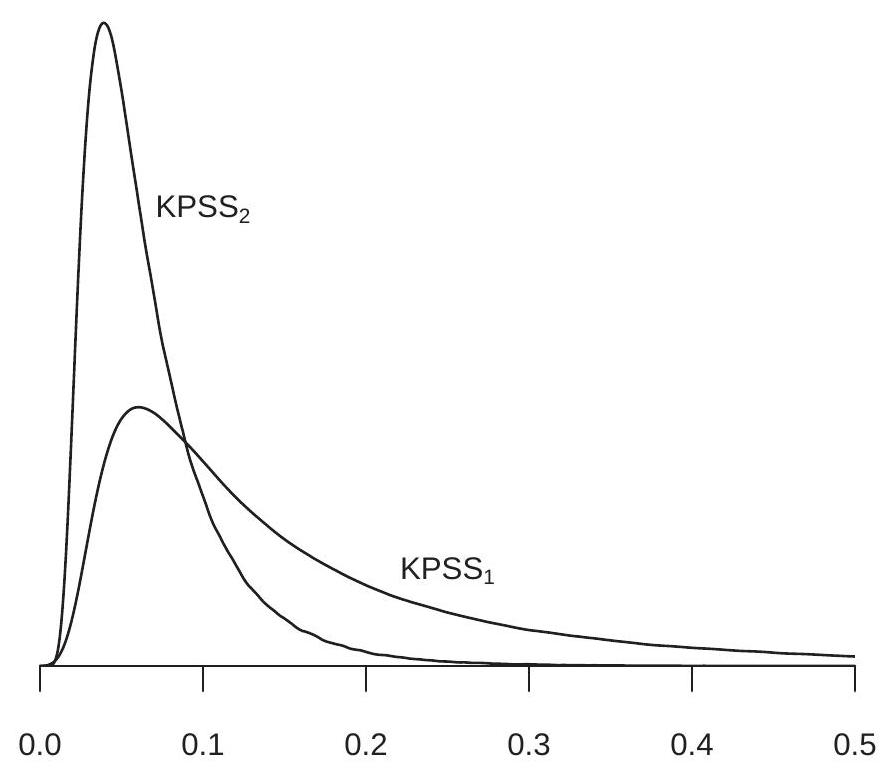
\includegraphics[max width=\textwidth]{2022_10_23_e99fc7c58db661c6f219g-24}

Figure 16.4: Density of KPSS Distribution

use a default rule based on a reasonable alternative. Suppose we consider the alternative $\rho=0.8$. The associated Andrews' reference rule is $M=3.1 n^{1 / 3}$. This leads to a simple rule $M=3 n^{1 / 3}$. An interpretation of this choice is that it should approximately control the size of the test when the truth is an AR(1) with coefficient $0.8$ but over-reject for more persistent AR processes.

To illustrate, Table $16.2$ reports the $\mathrm{KPSS}_{2}$ statistic for the same eight series as examined in the previous section, using $M=3 n^{1 / 3}$. For the first two quarterly series $n=228$ leading to $M=18$. For the six monthly series $n=684$ leading to $M=26$. For six of the eight series (all but consumption and the unemployment rate) the KPSS statistic equals or exceeds the $1 \%$ critical value leading to a rejection of the null hypothesis of stationarity in favor of the alternative of a unit root. This is consistent with the ADF test which failed to reject a unit root for these series.

For the consumption series the KPSS statistic has a p-value of $12 \%$, which does not reject the hypothesis of stationarity. Recall that the ADF test failed to reject the hypothesis of a unit root. Thus neither test leads to a decisive result; as a pair the two tests are inconclusive. In this context I recommend staying with the prediction of economic theory (consumption is a martingale) as it is not rejected by a hypothesis test. The KPSS fails to reject stationarity but that does not mean that the series is stationary.

An interesting case is the unemployment rate series. It has $\mathrm{KPSS}_{2}=0.14$ with a p-value of $6 \%$. This is borderline significant for rejection of stationarity. On the other hand, recall that the ADF test had a pvalue of $1 \%$ rejecting the unit root hypothesis. These results are borderline conflicting. To augment our information we calculate the KPSS $_{1}$ test as the unemployment rate does not appear to be trended. We find $\operatorname{KPSS}_{1}=0.19$ with a p-value of $30 \%$. This is clearly in the non-rejection region, failing to provide evi- dence against stationarity. As a whole, the ADF test (reject unit root), the $\mathrm{KPSS}_{1}$ test (accept stationarity), and the $\mathrm{KPSS}_{2}$ test (borderline reject stationarity), taken together are consistent with the interpretation that the unemployment rate is a stationary process.

The $\mathrm{KPSS}_{2}$ test can be implemented in Stata using the command ${ }^{7} \mathrm{kpss}$ y, $\operatorname{maxlag}(\mathrm{q})$. For the KPSS $_{1}$ test add the option notrend. The command reports the KPSS statistics for $M=1, \ldots, q$, as well as asymptotic critical values. Approximate asymptotic p-values are not reported.

\subsection{Spurious Regression}
One of the most empirically relevant discoveries from the theory of non-stationary time series is the phenomenon of spurious regression. This is the finding that two statistically independent series, if both unit root processes, are likely to fool traditional statistical analysis by appearing to be statistically related by both eyeball scrutiny and traditional statistical tests. The phenomenon was observed ${ }^{8}$ and named by Granger and Newbold (1974) and explained using the theory of non-stationary time series by Phillips (1986). The primary lesson is that it is easy to be tricked by non-stationary time-series but the problem disappears if we pay suitable attention to dynamic specification.

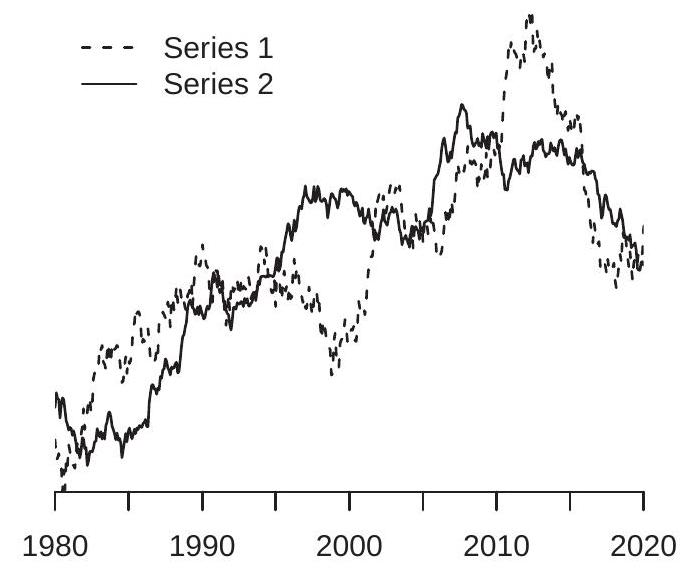
\includegraphics[max width=\textwidth]{2022_10_23_e99fc7c58db661c6f219g-25}

(a) Two Unrelated Random Walks

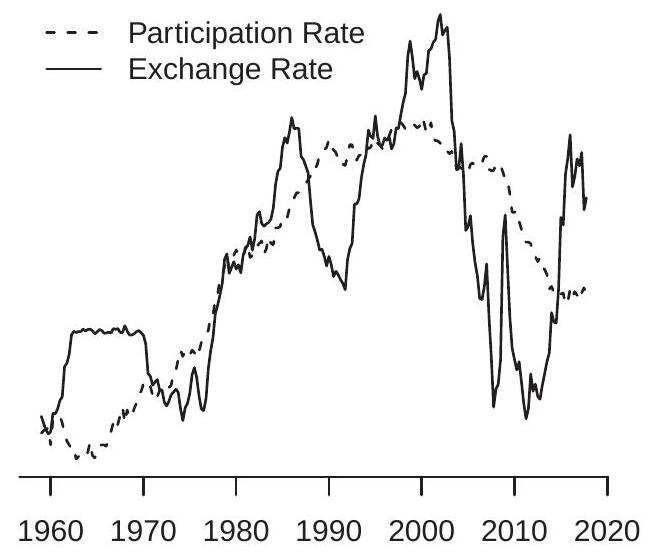
\includegraphics[max width=\textwidth]{2022_10_23_e99fc7c58db661c6f219g-25(1)}

(b) Exchange and Labor Force Participation Rates

Figure 16.5: Plots of Empirical Series

To illustrate the problem examine Figure 16.5(a). Displayed are two time series, monthly for 19802018. A casual review of the graphs shows that both series are generally increasing over 1980-2010 with a no-growth period around 2000, and the series display a downward trend for the final decade. A more refined perusal may appear to reveal that Series 2 leads Series 1 by about five years, in the sense that Series 2 reaches turning points about five years before Series 1. A casual observer is likely to deduce based on Figure 16.5(a) that the two time series are strongly related.

${ }^{7}$ The command kpss is not part of the standard package, but can be installed by typing ssc install kpss.

${ }^{8}$ In numerical simulations. However the truth is that Series 1 and Series 2 are statistically independent random walks generated by computer simulation, each standardized to have mean zero and unit variance for the purpose of visual comparison. The "fact" that both series are generally upward trended and have "similar" turning points are statistical accidents. Random walks have an uncanny ability to fool casual analysis. Newspaper (and other journalistic) articles containing plots of time series are routinely subject to the tricks of Figure 16.5(a). Economists are also routinely tricked and fooled.

Traditional statistical examination of the series in Figure 16.5(a) can also lead to a false inference of a strong relationship. A linear regression of Series 1 on Series 2 yields a slope coefficient of $0.76$ with classical standard error of $0.03$. The t-ratio for the test of a zero slope is $T=26$. The equation $R^{2}$ is $0.59$. These traditional statistics support the incorrect inference that the two series are strongly related.

Spurious relationships of this form are commonplace in economic time series. An example is shown in Figure 16.5(b), which displays the U.S. labor force participation rate and U.S.-Canada exchange rate, quarterly for 1960-2018. As a visual aid both series have been normalized to have mean zero and unit variance. Both series appear to grow at a similar rate from 1960-2000, though the exchange rate is more volatile. From 2000-2018 they reverse course, with both series declining. The visual evidence is supported by traditional statistics. A linear regression of labor participation on the exchange rate yields a slope coefficient of $0.70$ with a clasical standard error of $0.05$. The t-ratio for the test of a zero slope is $T=15$. The equation $R^{2}$ is $0.49$. The visual and statistical evidence support the inference that the two series are related.

This empirical "finding" that the labor participation and exchange rates are related does not make economic sense. Is this an example of a spurious regression between non-stationary variables? A visual inspection of each series supports the contention that each is non-stationary and may be well characterized as a unit root process. We saw in Sections $16.13$ and $16.14$ that the ADF and KPSS tests support the hypothesis that the exchange rate is a unit root process. Similar tests reach the same conclusion for labor force participation. Thus the two series are reasonably characterized as unit root processes and these two series could be an empirical example of a spurious regression.

For a formal framework assume that the series $Y_{t}$ and $X_{t}$ are random walk processes
$$
\begin{aligned}
Y_{t} &=Y_{t-1}+e_{1 t} \\
X_{t} &=X_{t-1}+e_{2 t}
\end{aligned}
$$
where $\left(e_{1 t}, e_{2 t}\right)$ are i.i.d., mean zero, mutually uncorrelated, and normalized to have unit variance. Let $Y_{t}^{*}$ and $X_{t}^{*}$ denote demeaned versions of $Y_{t}$ and $X_{t}$. From the FCLT they satisfy
$$
\left(\frac{1}{\sqrt{n}} Y_{\lfloor n r\rfloor}^{*}, \frac{1}{\sqrt{n}} X_{\lfloor n r\rfloor}^{*}\right) \underset{d}{\longrightarrow}\left(W_{1}^{*}(r), W_{2}^{*}(r)\right)
$$
where $W_{1}^{*}(r)$ and $W_{2}^{*}(r)$ are demeaned Brownian motions.

Applying the CMT the sample correlation has the asymptotic distribution
$$
\widehat{\rho}=\frac{\frac{1}{n^{2}} \sum_{i=1}^{n} Y_{i}^{*} X_{i}^{*}}{\left(\frac{1}{n^{2}} \sum_{i=1}^{n} Y_{i}^{* 2}\right)^{1 / 2}\left(\frac{1}{n^{2}} \sum_{i=1}^{n} X_{i}^{* 2}\right)^{1 / 2}} \underset{d}{\longrightarrow} \frac{\int_{0}^{1} W_{1}^{*} W_{2}^{*}}{\left(\int_{0}^{1} W_{1}^{* 2}\right)^{1 / 2}\left(\int_{0}^{1} W_{2}^{* 2}\right)^{1 / 2}} .
$$
The right-hand-side is a random variable. Furthermore it is also non-degenerate (indeed, it is non-zero with probability one). Thus the sample correlation $\widehat{\rho}$ remains random in large samples.

To understand magnitudes, Figure 16.6(a) displays the asymptotic distributon ${ }^{9}$ of $\widehat{\rho}$. The density has most probability mass in the interval $[-0.5,0.5]$, over which the density is essentially flat. This means that

${ }^{9}$ Calculated by simulation from one million simulation draws of samples of size $n=10,000$. the sample correlation has a diffuse distribution. Above we saw that the two simulated random walks had a sample correlation ${ }^{10}$ of $0.76$ and the two empirical series a sample correlation of $0.70$. We can now see that these results are consistent with the distribution shown in Figure 16.6(a) and are therefore uninformative regarding the underlying relationships.

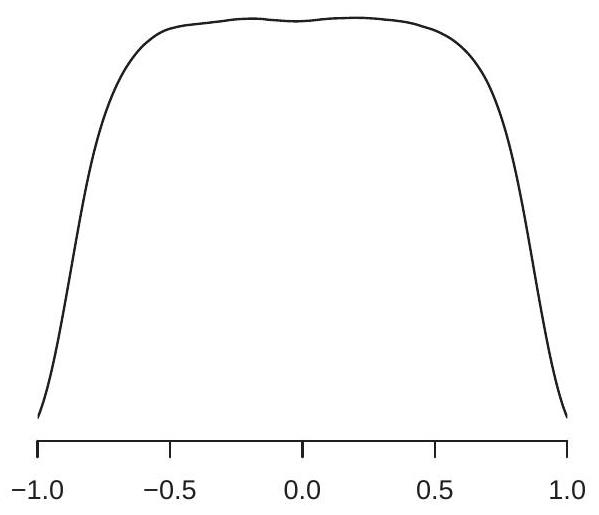
\includegraphics[max width=\textwidth]{2022_10_23_e99fc7c58db661c6f219g-27}

(a) Asymptotic Density of Sample Correlation

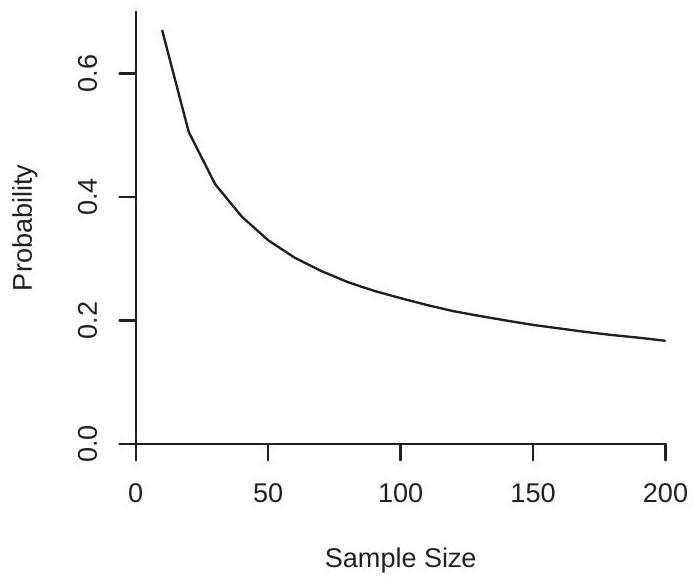
\includegraphics[max width=\textwidth]{2022_10_23_e99fc7c58db661c6f219g-27(1)}

(b) Coverage Probability of Nominal 95\% Interval

Figure 16.6: Properties of Spurious Regression

We can also examine the regression estimators. The slope coefficient from a regression of $Y_{t}$ on $X_{t}$ has the asymptotic distribution
$$
\widehat{\beta}=\frac{\frac{1}{n^{2}} \sum_{i=1}^{n} Y_{i}^{*} X_{i}^{*}}{\frac{1}{n^{2}} \sum_{i=1}^{n} X_{i}^{* 2}} \underset{d}{\longrightarrow} \frac{\int_{0}^{1} W_{1}^{*} W_{2}^{*}}{\int_{0}^{1} W_{2}^{* 2}} .
$$
This is a non-degenerate random variable. Thus the slope estimator remains random in large samples and does not converge in probability.

Now consider the classical t-ratio $T$. It has the asymptotic distribution
$$
\frac{1}{n^{1 / 2}} T=\frac{\frac{1}{n^{2}} \sum_{i=1}^{n} Y_{i}^{*} X_{i}^{*}}{\left(\frac{1}{n^{2}} \sum_{i=1}^{n} X_{i}^{* 2}\right)^{1 / 2}\left(\frac{1}{n^{2}} \sum_{i=1}^{n}\left(Y_{i}^{*}-X_{i}^{*} \widehat{\beta}\right)^{2}\right)^{1 / 2}} \underset{d}{\rightarrow} \frac{\int_{0}^{1} W_{1}^{*} W_{2}^{*}}{\left(\int_{0}^{1} W_{2}^{* 2}\right)^{1 / 2}\left(\int_{0}^{1}\left(W_{1}^{*}-W_{2}^{*} \frac{\int_{0}^{1} W_{1}^{*} W_{2}^{*}}{\int_{0}^{1} W_{2}^{* 2}}\right)^{2}\right)^{1 / 2}} .
$$
This is non-degenerate. Thus the $\mathrm{t}$-ratio has an asymptotic distribution only after normalization by $n^{1 / 2}$, meaning that the unnormalized t-ratio diverges in probability!

To understand the utter failure of classical inference theory observe that the regression equation is
$$
Y_{t}=\alpha+\beta X_{t}+\xi_{t}
$$
with true values $\alpha=0$ and $\beta=0$. This means that the error $\xi_{t}=Y_{t}$ is a random walk. The latter is considerably more strongly autocorrelated than allowed by stationary regression theory, invalidating conventional standard errors. The latter are too small by an order of magnitude resulting in t-ratios which are misleadingly large.

${ }^{10}$ Since the variables have been standardized to have a unit variance the sample correlation equals the least squares slope coefficient. What this means in practice is that $\mathrm{t}$-ratios from spurious regressions are random and large even when there is no relationship. This explains the large t-ratio $T=26$ for the simulated series and shows that the value $T=15$ for the empirical series is uninformative. The reason for a large t-ratio is not because the series are related but is rather because the series are unit root processes so classical standard errors mis-characterize estimation variance.

One of the features of the above theory is that it shows that the magnitude of the distortion of the t-ratio increases with sample size. Interestingly, the original Granger-Newbold (1974) analysis was a simulation study which confined attention to the case $n=50$. Granger-Newbold found the (then surprising) result that t-tests substantially overreject under the null hypothesis of a zero coefficient. It wasn't until the theoretical analysis by Phillips (1986) that it was realized that this distortion worsened as sample size increased. These results illustrate the insight - and limitations - of simulation analysis. Using simulation Granger-Newbold pointed out that there was a problem. But by fixing sample size at a single value they did not discover the surprising effect of sample size.

The fact that the t-ratio diverges as $n$ increases means that the coverage of classical confidence intervals worses as $n$ increases. To calibrate the magnitude of this distortion examine Figure 16.6(b). This plots ${ }^{11}$ the finite-sample coverage probability of classical nominal $95 \%$ confidence intervals for the slope using student $t$ critical values plotted as a function of sample size $n$. The observations were generated as independent random walks with normal innovations. You can see that the coverage ranges from $0.68$ (for $n=10$ ) to $0.2$ (for $n=200$ ). These coverage rates are unacceptably below the nominal coverage level of $0.95$

The above analysis focused on classical t-ratios and confidence intervals constructed with old-fashioned homoskedastic standard errors. This may seem to be an out-of-date analysis as we have made the case that old-fashioned standard errors are not used in contemporary econometric practice. However the problem as described carries over to alternative standard error constructions. The common heteroskedastic standard errors do not fundamentally change the asymptotic distribution. The Newey-West standard errors reduce the under-coverage but only partially. They are designed to consistently estimate the long-run variance of stationary series but fail when the series are non-stationary.

At this point let us collect what we have learned. If we have two time-series which are independent unit root processes, then by time-series plots, correlation analysis, and simple linear regressions it is easy to make the false inference that they are related. Their sample correlations and regression slope estimates will be random, inconsistent, and uninformative.

Our deduction is that it is inappropriate to use simple inference techniques when handling potentially non-stationary time series. We need to be more careful and use better inference methods.

It turns out that a simple modification is often sufficient to fundamentally alter the inference problem. Again, suppose we observe the independent series (16.10)-(16.11). A linear regression model is (16.12) with error $\xi_{t}=Y_{t}$. We can write the latter as $\xi_{t}=Y_{t-1}+e_{t}$. This means that a correct dynamic specfication of the regression model is
$$
Y_{t}=\alpha+\beta X_{t}+\delta Y_{t-1}+e_{t}
$$
with $\alpha=\beta=0$ and $\delta=1$. If equation (16.13) is estimated the error is no longer a random walk and inference on $\beta$ can proceed conventionally! In this simple example a solution is simply to include the lagged dependent variable $Y_{t-1}$ in the estimated regression. More generally, if a trend component is missing or $\Delta Y_{t}$ is serially correlated it is necessary to include the trend terms and/or sufficient lags of $Y_{t}$ in the estimated regression.

For example, take the simulated random walk series from Figure 16.5(a). Estimating model (16.13) we find $\widehat{\beta}=0.004$ with a standard error of $0.005$. Thus by adding the lagged dependent variable the

${ }^{11}$ Calculated by simulation on a grid of values for $n$ with one million simulation replications. spurious regression relationship has been broken. Now take the empirical series from Figure 16.5(b). We estimate an analog of (16.13) augmented with a linear trend. The estimate of $\beta$ in this model is $0.16$ with a standard error of $0.12$. Once again the spurious regression relationship has been broken by a simple dynamic re-adjustment.

This seems like a straightforward solution. If so, why does the spurious regression problem persist ${ }^{12}$ in applied analysis? The reason is partially that non-specialists find that the simple regression (16.12) is easy to interpret while the dynamic model (16.13) is challenging to interpret. One of the tasks of a skilled econometrician is to understand this failure of reasoning, to explain the problem to colleagues and users, and to present constructive useful alternative methods of analysis.

\subsection{NonStationary VARs}
Let $Y_{t}$ be an $m \times 1$ time series. Suppose that $Y_{t}$ satisfies a VAR(p-1) in first differences, thus $\boldsymbol{D}(\mathrm{L}) \Delta Y_{t}=$ $e_{t}$ where $\boldsymbol{D}(z)$ is invertible and $\Sigma=\operatorname{var}\left[e_{t}\right]>0$. Then $\Delta Y_{t}$ has the long-run covariance matrix $\Omega=$ $\boldsymbol{D}(1)^{-1} \Sigma \boldsymbol{D}(1)^{-1 \prime}>0$. In this case $Y_{t}$ is a vector $I(1)$ process in the sense that each element of $Y_{t}$ is $I(1)$ and so are all linear combinations of $Y_{t}$.

The model can be written as a VAR in levels as
$$
Y_{t}=\boldsymbol{A}_{1} Y_{t-1}+\boldsymbol{A}_{2} Y_{t-2}+\cdots+\boldsymbol{A}_{p} Y_{t-p}+e_{t}
$$
where $\boldsymbol{A}_{1}+\boldsymbol{A}_{2}+\cdots+\boldsymbol{A}_{p}=\boldsymbol{I}_{m}$. It can also be written in the mixed format
$$
\Delta Y_{t}=\boldsymbol{A} Y_{t-1}+\boldsymbol{D}_{1} \Delta Y_{t-1}+\cdots+\boldsymbol{D}_{p-1} \Delta Y_{t-p+1}+e_{t}
$$
where $\boldsymbol{A}=0$. These are equivalent algebraic representations. Let $d=\operatorname{vec}\left(\left(\boldsymbol{D}_{1}, \ldots, \boldsymbol{D}_{p-1}\right)^{\prime}\right)$.

Let $(\widehat{\boldsymbol{A}}, \widehat{d})$ be the multivariate least squares estimator of (16.15). Set $X_{t}=\left(\Delta Y_{t-1}, \ldots, \Delta Y_{t-p+1}\right)$.

Theorem 16.16 Assume that $\Delta Y_{t}$ follows the $\operatorname{VAR}(\mathrm{p}-1)$ process $\boldsymbol{D}(\mathrm{L}) \Delta Y_{t}=e_{t}$ with invertible $\boldsymbol{D}(z), \mathbb{E}\left[e_{t} \mid \mathscr{F}_{t-1}\right]=0, \mathbb{E}\left\|e_{t}\right\|^{4}<\infty$, and $\mathbb{E}\left[e_{t} e_{t}^{\prime}\right]=\Sigma>0$. Then as $n \rightarrow \infty$
$$
\left(\begin{array}{c}
n \widehat{\boldsymbol{A}} \\
\sqrt{n}(\widehat{d}-d)
\end{array}\right) \underset{d}{\longrightarrow}\left(\begin{array}{c}
\Sigma^{1 / 2} \int_{0}^{1} d W W^{\prime}\left(\int_{0}^{1} W W^{\prime}\right)^{-1} \Omega^{-1 / 2} \\
\mathrm{~N}(0, \boldsymbol{V})
\end{array}\right)
$$
where $W(r)$ is vector Brownian motion and
$$
\begin{aligned}
&\boldsymbol{V}=\left(\boldsymbol{I}_{m} \otimes \mathbb{E}\left[X_{t} X_{t}^{\prime}\right]\right)^{-1} \Omega\left(\boldsymbol{I}_{m} \otimes \mathbb{E}\left[X_{t} X_{t}^{\prime}\right]\right)^{-1} \\
&\Omega=\mathbb{E}\left[e_{t} e_{t}^{\prime} \otimes X_{t} X_{t}^{\prime}\right] .
\end{aligned}
$$
The top component of the asymptotic distribution is a multivariate version of the Dickey-Fuller coefficient distribution. The bottom component is a conventional normal distribution. This shows that the

${ }^{12}$ An amusing exercise is to peruse newspaper/magazine articles for time series plots of historical series. More often than not the displayed series appear to be $I(1)$, and more often than not the article describes the series as "related" based on a combination of eyeball analysis and simple correlation statistics. coefficient estimator $\widehat{\boldsymbol{A}}$ is consistent at the $O_{p}\left(n^{-1}\right)$ rate, converges to a non-standard (biased and nonnormal) asymptotic distribution, and the coefficient estimator $\widehat{d}$ has a conventional asymptotic normal distribution.

Parameters of interest, including the coefficients of the levels equation (16.14), impulse response functions, and forecast error decompositions, are linear combination of the estimators $(\widehat{\boldsymbol{A}}, \widehat{d})$. For $\operatorname{VAR}(\mathrm{p})$ models with $p \geq 2$, unless the linear combination of interest is in the span of $\widehat{A}$, the asymptotic distribution of estimators are dominated by the $O_{p}\left(n^{-1 / 2}\right)$ component $\widehat{d}$. Thus these coefficient estimators have conventional asymptotic normal distributions. Consequently, for most purposes estimation and inference on a VAR model is robust to the presence of (multivariate) unit roots.

There are two important exceptions. First, inference on the sum of levels coefficients $A_{1}+A_{2}+\cdots+A_{p}$ is non-standard as the estimator of this sum has the multivariate Dickey-Fuller coefficient distribution. This includes questions concerning the presence of unit roots and many questions concerning the longrun properties of the series. Second, the long-run impulse matrix $C=A^{-1}=\left(I-A_{1}-A_{2}-\cdots-A_{p}\right)^{-1}$ is a (non-linear) function of this same sum and thus by the Delta Method is asymptotically a linear transformation of the multivariate Dickey-Fuller coefficient distribution. This means that the least squares estimator of $\boldsymbol{C}$ is non-standard (biased and non-normal). As $\boldsymbol{C}$ is the limit of the CIRF as the horizon tends to infinity this indicates that estimators of the CIRF at long horizons will be non-standard in finite samples. Consequently when a VAR model includes variables which are potentially unit root processes the conventional confidence intervals for the CIRF at long horizons are not trustworthy. This is a widespread issue since macroeconomists routinely estimate VAR models with macroeconomic variables in levels (for example, the Blanchard-Perotti (2002) model presented in Section 15.25).

\subsection{Cointegration}
A fascinating topic is cointegration. The idea is due to Granger (1981) and was articulated in detail by Engle and Granger (1987). A pair of unit root processes are cointegrated if their difference (or some linear combination) is stationary. This means that the pair "hang together" over the long run.

To visualize, examine Figure 16.7(a). This shows two interest rate series. The solid line is the interest rate (quarterly for 1959-2017) on ten-year U.S. Treasury Bonds ${ }^{13}$. The dashed line is the interest rate on 3-month U.S. Treasury Bonds ${ }^{14}$. Over the 59-year period the two series move up and down together. The 10-year rate exceeds the 3-month rate in most time periods. For some periods the two lines pull apart but they always come together again. This indicates that the two time series are tightly tied together. From our unit root analysis we have already determined that the 10-year interest rate is consistent with a unit root process; the same findings apply to the 3-month series. Thus it appears that these are two time series which are individually unit root processes but jointly track each other closely.

To see this further define the interest rate spread as the difference between the two interest rates, long (10-year) minus short (3-month). This series is plotted in Figure 16.7(b). The mean of the series is displayed by the dashed line. What we can see is that the spread roughly appears to be mean reverting. With the possible exception of the first decade of the plot we see that that the spread crosses its mean multiple times each decade. The fluctuations appear to be stationary. Applying an ADF unit root test with no trend included to the spread yields $\mathrm{ADF}=-4.0$ which is less than the $1 \%$ critical value, rejecting the null hypothesis of a unit root. Thus the levels of the two interest rates appear to be non-stationary while the spread is stationary. This suggests that the two interest rate series are cointegrated.

This concept is formalized in the following definition.

${ }^{13}$ From FRED-QD, series gs10.

${ }^{14}$ From FRED-QD, series tb3ms.

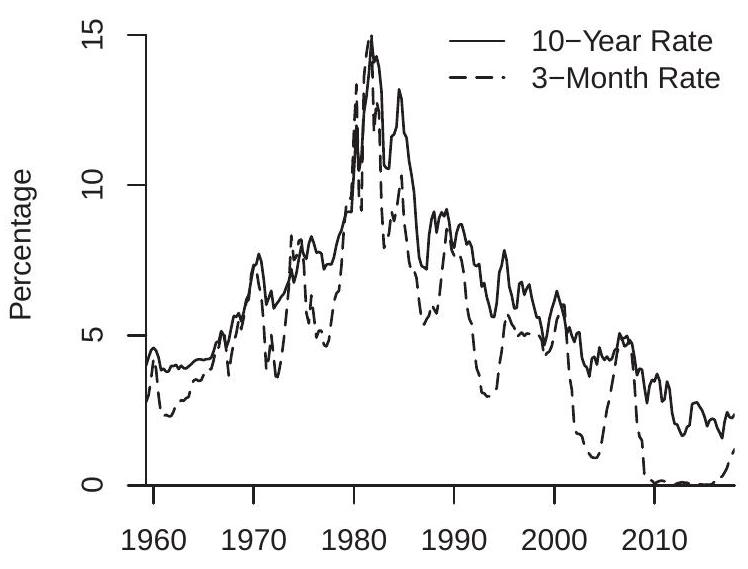
\includegraphics[max width=\textwidth]{2022_10_23_e99fc7c58db661c6f219g-31}

(a) Interest Rates

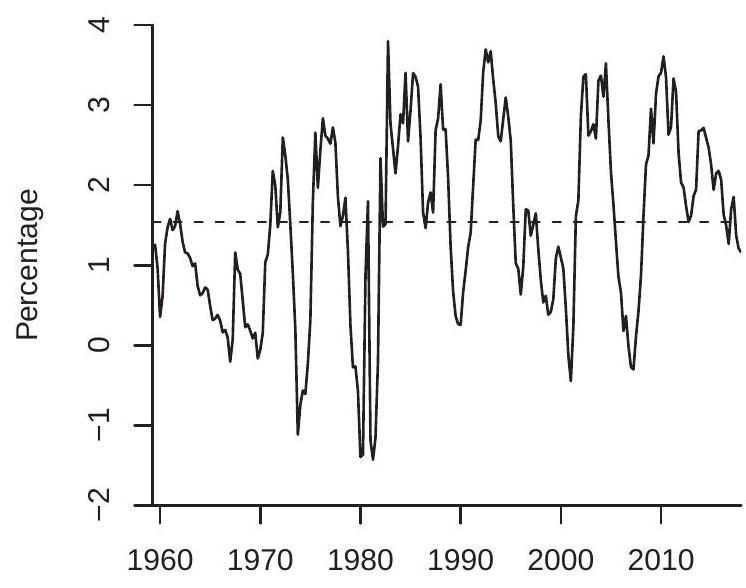
\includegraphics[max width=\textwidth]{2022_10_23_e99fc7c58db661c6f219g-31(1)}

(b) Interest Rate Spread

Figure 16.7: Cointegration

Definition 16.5 The $m \times 1$ non-deterministic series $Y_{t}$ is cointegrated if there exists a full rank $m \times m$ matrix $\left[\beta, \beta_{\perp}\right]$ such that $\beta^{\prime} Y_{t} \in \mathbb{R}^{r}$ and $\beta_{\perp}^{\prime} \Delta Y_{t} \in \mathbb{R}^{m-r}$ are $I(0)$. The $r$ vectors in $\beta$ are called the cointegrating vectors. The variable $Z_{t}=\beta^{\prime} Y_{t}$ is called the equilibrium error.

In the interest rate example of Figure 16.7, there are $m=2$ series and $r=1$ cointegrating relationships. Our discussion assumes that the cointegrating vector is $\beta=(1,-1)^{\prime}$.

The cointegrating vectors $\beta$ are not individually identified; only the space spanned by the vectors is identified so $\beta$ is typically normalized. When $r=1$ a common normalization is to set one non-zero element equal to one. Another common normalization is to set $\beta$ to be orthonormal: $\beta^{\prime} \beta=\boldsymbol{I}_{r}$. Theorem 16.17 Granger Representation Theorem. If non-deterministic $Y_{t} \in$ $\mathbb{R}^{m}$ is cointegrated with $m \times r$ cointegrating vectors $\beta$ and (16.1) holds, then

\begin{enumerate}
  \item The coefficients of the Wold representation
\end{enumerate}
$$
\Delta Y_{t}=\theta+\Theta(\mathrm{L}) e_{t}
$$
satisfy $\Theta(1)=\beta_{\perp} \eta^{\prime}$ and $\theta=\beta_{\perp} \gamma$ for some full-rank $m \times(m-r)$ matrix $\eta$ and some $(m-r) \times 1 \gamma$.

\begin{enumerate}
  \setcounter{enumi}{2}
  \item The Beveridge-Nelson decomposition of $Y_{t}$ is
\end{enumerate}
$$
Y_{t}=\beta_{\perp}\left(\gamma t+\eta^{\prime} S_{t}\right)+U_{t}+V_{0}
$$
where $S_{t}=\sum_{i=1}^{t} e_{t}, U_{t}=\Theta^{*}(\mathrm{~L}) e_{t}$ is a stationary linear process, and $V_{0}=$ $Y_{0}-U_{0}$ is an initial condition.

\begin{enumerate}
  \setcounter{enumi}{3}
  \item Suppose that (a) all complex solutions to $\operatorname{det}(\Theta(z))=0$ are either $z=1$ or $|z| \geq 1+\delta$ for some $\delta>0$; (b) $\beta^{\prime} \Theta^{*}(1) \eta_{\perp}$ is full rank, where $\eta_{\perp}$ is a full rank $m \times r$ matrix such that $\eta^{\prime} \eta_{\perp}=0$. Then $Y_{t}$ has the (infinite-order) convergent VAR representation
\end{enumerate}
$$
\boldsymbol{A}(\mathrm{L}) Y_{t}=a+e_{t}
$$
where the coefficients satisfy $\boldsymbol{A}(1)=-\eta_{\perp}\left(\beta^{\prime} \Theta^{*}(1) \eta_{\perp}\right)^{-1} \beta^{\prime}$. All complex solutions to $\operatorname{det}(\boldsymbol{A}(z))=0$ are either $z=1$ or $|z| \geq 1+\delta$ for some $\delta>0$.

\begin{enumerate}
  \setcounter{enumi}{4}
  \item Under the assumptions of part 3 plus $\sum_{j=0}^{\infty}\left\|\sum_{k=0}^{\infty} k \Theta_{j+k}\right\|^{2}<\infty$ the VAR representation can be written in error-correction form
\end{enumerate}
$$
\Delta Y_{t}=\alpha \beta^{\prime} Y_{t-1}+\Gamma(\mathrm{L}) \Delta Y_{t-1}+a+e_{t}
$$
where $\Gamma(\mathrm{L})$ is a lag polynomial with absolutely summable coefficient matrices and $\alpha=-\eta_{\perp}\left(\beta^{\prime} \Theta^{*}(1) \eta_{\perp}\right)^{-1}$.

\begin{enumerate}
  \setcounter{enumi}{5}
  \item If $\theta=0$ in the Wold representation (16.16) then $\gamma=0$ in (16.17) so there is no linear trend in (16.17). The intercept in (16.18) and (16.19) equals $a=\alpha \mu$ where $\mu$ is $r \times 1$. Equation (16.19) can be written as
\end{enumerate}
$$
\Delta Y_{t}=\alpha\left(\beta^{\prime} Y_{t-1}+\mu\right)+\Gamma(\mathrm{L}) \Delta Y_{t-1}+e_{t} .
$$
The proof is presented in Section 16.22. The Granger Representation Theorem appears in Engle and Granger (1987). The assumption on $\beta^{\prime} \Theta^{*}(1) \eta_{\perp}$ was introduced by Johansen (1995, Theorem 4.5).

Part 1 shows that the coefficients of the Wold representation sum to a singular matrix in the null space of the cointegrating vectors.

Part 2 gives the Beveridge-Nelson permanent-transitory representation of $Y_{t}$. It shows that the trend $\beta_{\perp}\left(\gamma t+\eta^{\prime} S_{t}\right)$ lies in the null space of the cointegrating vectors. Thus there is no trend in the range space of the cointegrating vectors. This shows that the cointegrated vector $Y_{t}$ can be thought of as possessing $r$ "unit roots and linear trends" and $m-r$ "stationary processes". Part 3 provides the VAR representation. It shows that the VAR coefficients sum to a singular matrix which is in the range space of the cointegrating vectors.

Part 4 is perhaps the most famous result. It shows that a cointegrated system satisfies equation (16.19) which is called the error-correction representation. The error-correction representation is a regression model in stationary transformations as the variables $\Delta Y_{t}$ and $\beta^{\prime} Y_{t-1}$ are stationary. The equation shows that the change $\Delta Y_{t}$ relates to past changes $\Delta Y_{t-1}$ (as in a standard VAR) as well as the equilibrium error $\beta^{\prime} Y_{t-1}$. The full term $\alpha \beta^{\prime} Y_{t-1}$ is known as the "error-correction term". It is the key component which governs how the cointegrated relationship is maintained.

Part 5 examines the case of no linear trend. The condition $\theta=0$ arises when the variables $\Delta Y_{t}$ are all mean zero. The theorem (unsuprisingly) shows that this implies that the linear trend does not appear in the Beveridge-Nelson decomposition. More interestingly the theorem shows that this condition implies that the error-correction model can be written to incorporate the intercept.

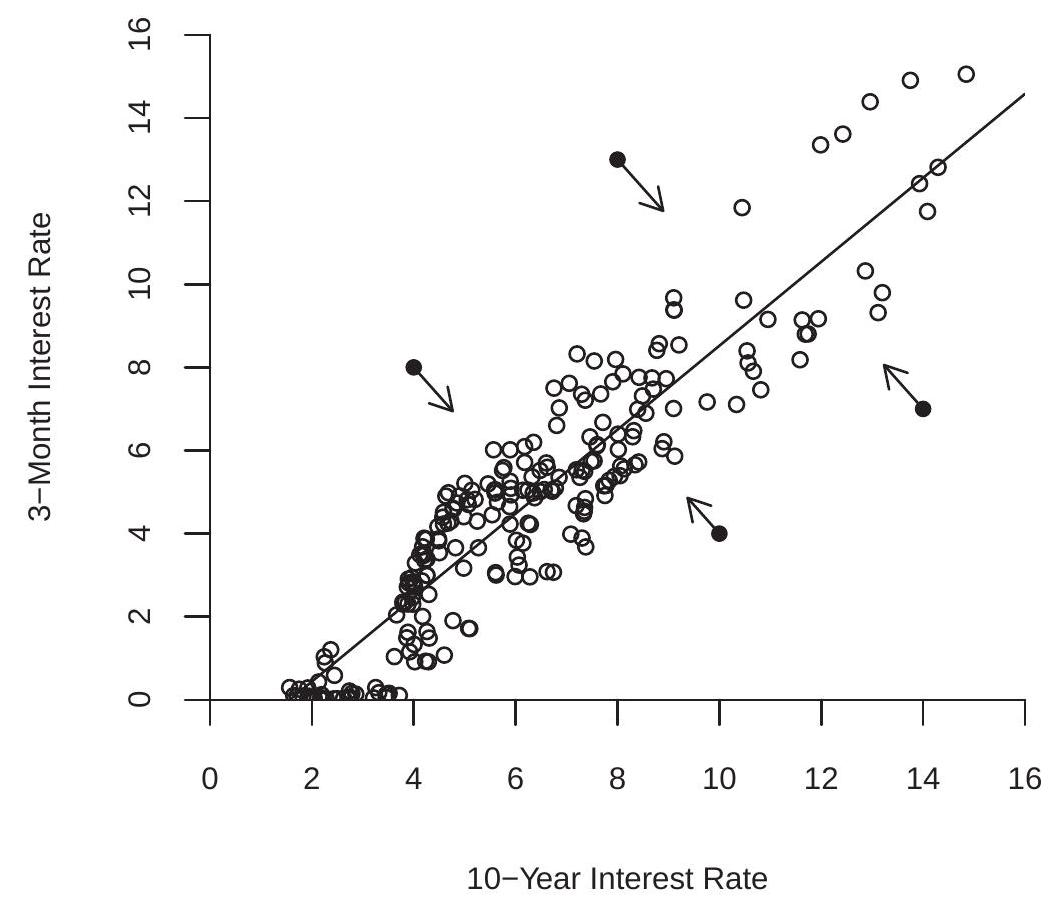
\includegraphics[max width=\textwidth]{2022_10_23_e99fc7c58db661c6f219g-33}

Figure 16.8: Error Correction Effect

To understand the error-correction effect examine Figure 16.8. This shows a scatter plot of the historical values of the two interest rate series from Figure 16.7. Also plotted is an estimate ${ }^{15}$ of the linear relation $\beta^{\prime} Y+\mu$ displayed as the solid line. This is the attractor of the system. For values of $Y$ on this line $\beta^{\prime} Y+\mu=0$. For values to the southeast $\beta^{\prime} Y+\mu<0$, and for values to the northwest $\beta^{\prime} Y+\mu>0$. The components of $\alpha$ dictate how these values impact the expected direction of $\Delta Y$. The arrows indicate these directions ${ }^{16}$. When $\beta^{\prime} Y+\mu>0$ the error correction decreases the 3-month rate and increases the

${ }^{15}$ From Table $16.4$

${ }^{16}$ From the estimates in Table $16.5$. 10-year rate, pushing $Y$ towards the line of attraction. When $\beta^{\prime} Y+\mu<0$ the error correction increases the 3-month rate and decreases the 10-year rate, again pushing $Y$ towards the line of attraction. In this particular example the two effects are similar in magnitude so the arrows show that both variables move towards the attractor in response to deviations.

Theorem $16.17$ shows that if $Y_{t}$ is cointegrated then it satisfies a VECM. The reverse is also the case.

Theorem 16.18 Granger Representation Theorem, Part II. Suppose that $Y_{t}$ satisfies a $\operatorname{VAR}(\infty)$ model $\boldsymbol{A}(\mathrm{L}) Y_{t}=a+e_{t}$ with $\operatorname{VECM}$ representation
$$
\Delta Y_{t}=\alpha \beta^{\prime} Y_{t-1}+\Gamma(\mathrm{L}) \Delta Y_{t-1}+a+e_{t}
$$
where $\beta$ and $\alpha$ are $m \times r$ and full rank. Suppose that (a) All complex solutions to $\operatorname{det}(\boldsymbol{A}(z))=0$ are either $z=1$ or $|z| \geq 1+\delta$ for some $\delta>0$; (b) $\sum_{j=0}^{\infty}\left\|\Gamma_{j}\right\|<\infty$; (c) $\alpha_{\perp}^{\prime}\left(\boldsymbol{I}_{m}-\Gamma(1)\right) \beta_{\perp}$ is full rank where $\alpha_{\perp}$ and $\beta_{\perp}$ lie in the null spaces of $\alpha$ and $\beta$. Then $Y_{t}$ is cointegrated with cointegrating vectors $\beta$.

The proof is presented in Section 16.22. This result for a finite-order VAR first appeared in Johansen (1995, Theorem 4.2).

The condition that $\alpha_{\perp}^{\prime} \Gamma(1) \beta_{\perp}$ is full rank is necessary to exclude the (somewhat pathological) possibility that the system is "multi-cointegrated", meaning that a linear combination of $\beta^{\prime} Y_{t-1}$ and $\Delta Y_{t-1}$ is of reduced order of integration. Together, Theorems $16.17$ and $16.18$ show that a VECM representation is necessary and sufficient for a vector time series to be cointegrated.

\subsection{Role of Intercept and Trend}
The role of intercepts and trends in cointegrating VECMs gives rise to distinct models. We list some major options.

\begin{enumerate}
  \item Trend Model 1. This specification has no intercept or trend terms
\end{enumerate}
$$
\Delta Y_{t}=\alpha \beta^{\prime} Y_{t-1}+\Gamma(\mathrm{L}) \Delta Y_{t-1}+e_{t} .
$$
This is convenient for pedagogy but is not relevant for empirical applications. In Stata use option trend (none).

\begin{enumerate}
  \setcounter{enumi}{2}
  \item Trend Model 2. This specification is appropriate for non-trended series such as interest rates. In this model the intercept is in the cointegrating relationship
\end{enumerate}
$$
\Delta Y_{t}=\alpha\left(\beta^{\prime} Y_{t-1}+\mu\right)+\Gamma(\mathrm{L}) \Delta Y_{t-1}+e_{t} .
$$
In Stata use option trend (rconstant).

\begin{enumerate}
  \setcounter{enumi}{3}
  \item Trend Model 3. This is appropriate for series which have possible linear trends. This model has an unconstrained intercept
\end{enumerate}
$$
\Delta Y_{t}=\alpha \beta^{\prime} Y_{t-1}+\Gamma(\mathrm{L}) \Delta Y_{t-1}+a+e_{t} .
$$
In this model the level series $Y_{t}$ is the sum of a linear time trend and a unit root process. The equilibrium error $\beta^{\prime} Y_{t}$ is stationary so eliminates the linear time trend and the unit root component. In Stata use option trend (constant). 4. Trend Model 4. This model extends the VECM model to allow a linear trend in the cointegrating relationship. This model is
$$
\Delta Y_{t}=\alpha\left(\beta^{\prime} Y_{t-1}+\mu t\right)+\Gamma(\mathrm{L}) \Delta Y_{t-1}+a+e_{t} .
$$
In this model the level series $Y_{t}$ is the sum of a linear time trend and a unit root process. The equilibrium error $\beta^{\prime} Y_{t}$ contains a linear time trend and a stationary process. Thus the cointegrating vector $\beta$ only eliminates the unit root, not the time trend component. In Stata use option trend (rtrend).

\begin{enumerate}
  \setcounter{enumi}{5}
  \item Trend Model 5. This is a further extension allowing an unconstrained trend term
\end{enumerate}
$$
\Delta Y_{t}=\alpha \beta^{\prime} Y_{t-1}+\Gamma(\mathrm{L}) \Delta Y_{t-1}+a+b t+e_{t} .
$$
In this model the unconstrained trend induces a quadratic time trend into the levels series $Y_{t}$. This is not a typical modeling choice for applied economic time series. In Stata use option trend (trend).

\subsection{Cointegrating Regression}
If $Y_{t}$ is cointegrated with a single cointegrating vector $(r=1)$ then it turns out that $\beta$ can be estimated by a least squares regression of one component of $Y_{t}$ on the others. This approach may be fruitfully employed when the major focus is the cointegrating vector, the number of variables $m$ is small (e.g. $m=2$ or $m=3$ ), and it is known that the number of cointegrating vectors $r$ is at most one.

Partition $Y_{t}=\left(Y_{1 t}, Y_{2 t}\right)$ and reparameterize $\beta$ as $(1,-\beta)$. Thus the first component of the cointegrating vector has been normalized to one (this requires that the true value is non-zero) and the remainder multiplied by $-1$. The coefficient of interest is $\beta$. Least squares is fit either to the equation
$$
Y_{1 t}=\mu+\beta^{\prime} Y_{2 t}+u_{1 t}
$$
(for Trend Models 1 or 2 ) or to the equation
$$
Y_{1 t}=\mu+\theta t+\beta^{\prime} Y_{2 t}+u_{1 t}
$$
(for Trend Models 3 or 4 ).

Define $u_{2 t}=\Delta Y_{2 t}, u_{t}=\left(u_{1 t}, u_{2 t}^{\prime}\right)^{\prime}$, and the long-run covariance matrix $\Omega=\Sigma+\Lambda+\Lambda^{\prime}$ where $\Sigma=$ $\mathbb{E}\left[u_{t} u_{t-\ell}^{\prime}\right]$ and $\Lambda=\sum_{\ell=1}^{\infty} \mathbb{E}\left[u_{t-\ell} u_{t}^{\prime}\right]$. Partition the covariance matrices conformably with $Y$, e.g.
$$
\Omega=\left[\begin{array}{ll}
\Omega_{11} & \Omega_{12} \\
\Omega_{21} & \Omega_{22}
\end{array}\right] .
$$
Theorem $16.19$ If $u_{t}$ satisfies the conditions of Theorem $16.4$ and $\Omega_{22}>0$ then the least squares estimator satisfies
$$
n(\widehat{\beta}-\beta) \underset{d}{\longrightarrow}\left(\int_{0}^{1} X X^{\prime}\right)^{-1}\left(\int_{0}^{1} X d B_{1}+\Sigma_{21}+\Lambda_{21}\right)
$$
where $B(r)=\left(B_{1}(r), B_{2}(r)\right)$ is a vector Brownian motion with covariance matrix $\Omega$ and $X(r)$ is determined by the model:

Trend Model 1 or 2 estimated by $(16.21): X=B_{2}^{*}$ (demeaned $B_{2}(r)$ ).

Trend Model 3 or 4 estimated by (16.22): $X=B_{2}^{* *}$ (detrended $\left.B_{2}(r)\right)$. The proof is presented in Section $16.22$.

Theorem $16.19$ shows that the estimator converges at the superconsistent $O_{p}\left(n^{-1}\right)$ rate. This was discovered by Stock (1987) and the asymptotic distribution derived by Park and Phillips (1988). The asymptotic distribution is non-standard due to the serial correlation terms. Take our empirical example. A least squares regression of the 3-month interest rate on the 10-year interest rate yields the estimated equation $\widehat{Y}_{1 t}=1.03 Y_{2 t}-1.71$.

Modifications to the least squares estimator which eliminate the non-standard components were introduced by Phillips and B. E. Hansen (1990) and Stock and Watson (1993). The Phillips-Hansen estimator, known as Fully Modified OLS (FM-OLS), eliminates the non-standard components through first-stage estimation of the serial correlation terms. The Stock-Watson estimator, known as Dynamic OLS (DOLS), eliminates the non-standard components by estimating an augmented regression including leads and lags of $\Delta Y_{2 t}$.

We are often interested in testing the hypothesis of no cointegration:
$$
\begin{aligned}
&\mathbb{H}_{0}: r=0 \\
&\mathbb{H}_{1}: r>0 .
\end{aligned}
$$
Under $\mathbb{H}_{0}, Z_{t}=\beta^{\prime} Y_{t}$ is $I(1)$ yet under $\mathbb{H}_{1} Z_{t}$ is $I(0)$. When $\beta$ is known $\mathbb{H}_{0}$ can be tested by appying a univariate ADF test on $Z_{t}$. Take the interest rate example. We already conjectured that the interest rate spread is stationary which is the same as the hypothesis that $\beta=1$ is the cointegrating coefficient. Using this value we computed $\mathrm{ADF}=-4.0$ with an asymptotic $\mathrm{p}$-value less than $0.01$. Hence we are able to reject the null hypothesis of a unit root in the spread, or equivalently reject the null hypothesis of no cointegration.

When $\beta$ is unknown, Engle and Granger (1987) proposed testing the null hypothesis of no cointegration by applying the ADF test to the least squares residual $\widehat{u}_{1 t}$ from either (16.21) or (16.22). The asymptotic null distribution is different from the Dickey-Fuller distribution since under $\mathbb{M}_{0}$ the estimated regression is spurious so the least squares estimator is inconsistent. The asymptotic distribution of the statistic was worked out by Phillips and Ouliaris (1990) by combining the theory of spurious regression with Dickey-Fuller distribution theory. Let $\mathrm{EG}_{p}$ denote the Engle-Granger ADF statistic with $p$ autoregressive lags in the ADF regression.

Theorem 16.20 Assume that $\left(\Delta Y_{1 t}, \Delta Y_{2 t}\right)$ satisfies the conditions of Theorem $16.4$ and $\Omega>0$. If $p \rightarrow \infty$ as $n \rightarrow \infty$ such that $p^{3} / n \rightarrow 0$ then
$$
\mathrm{EG}_{p} \underset{d}{\rightarrow} \frac{\left(\int_{0}^{1} V d V\right)}{\left(\int_{0}^{1} V^{2}\right)^{1 / 2}\left(1+\zeta^{\prime} \zeta^{1 / 2}\right.}
$$
where, $V(r)=W_{1}^{*}(r)-\zeta^{\prime} W_{2}^{*}(r)$ and $\zeta=\left(\int_{0}^{1} W_{2}^{*} W_{2}^{* \prime}\right)^{-1}\left(\int_{0}^{1} W_{2}^{*} W_{1}^{*}\right), W(r)=$ $\left(W_{1}(r), W_{2}(r)\right)$ is vector standard Brownian motion, and $W^{*}(r)$ is demeaned $W(r)$ if $(16.21)$ is estimated or detrended $W(r)$ if $(16.22)$ is estimated.

For a proof see Phillips and Ouliaris (1990).

An unusual feature of this Theorem is that it requires $p \rightarrow \infty$ as $n \rightarrow \infty$ even if the true process is a finite order AR process because the first stage spurious regression induces serial correlation into the first-stage residuals which needs to be handled in the second stage ADF test. Another unusual feature is the component $1+\zeta^{\prime} \zeta$ in the denominator. This is due to the variance estimator component which asymptotically is random because of the first stage spurious regression.

Table 16.3: Engle-Granger Cointegration Test Critical Values

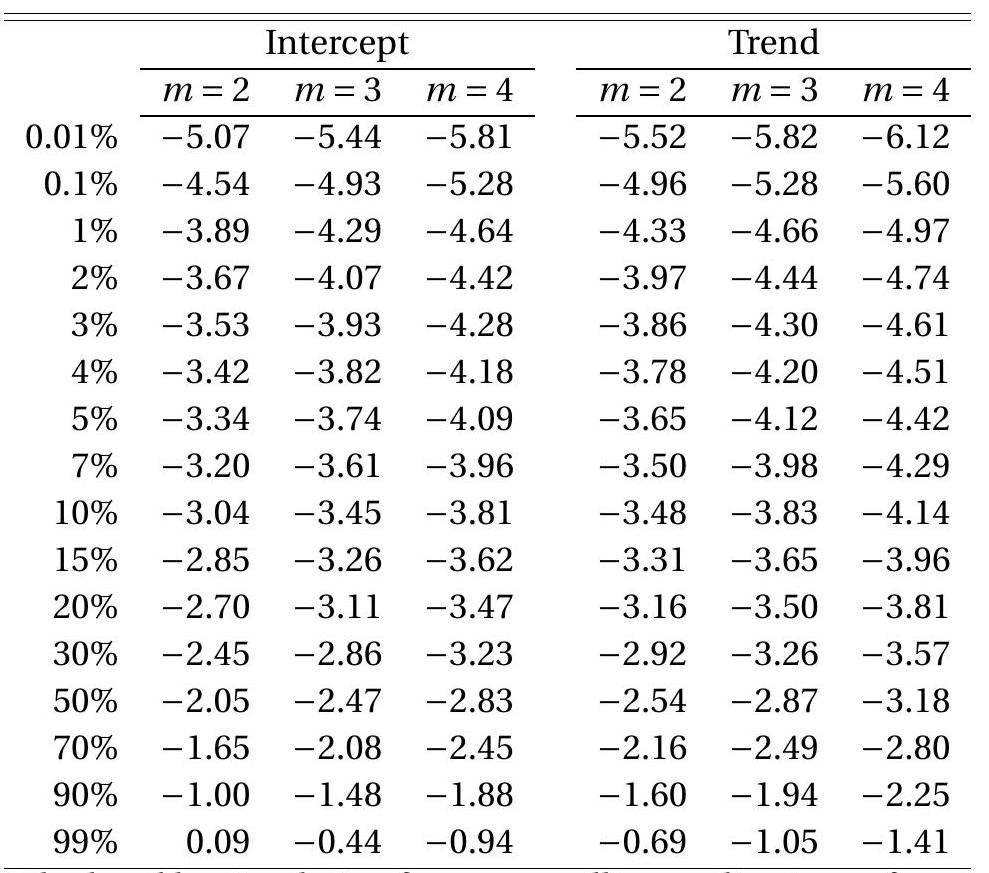
\includegraphics[max width=\textwidth]{2022_10_23_e99fc7c58db661c6f219g-37}

Source: Calculated by simulation from one million replications of samples of size $n=10,000$.

The asymptotic critical values ${ }^{17}$ are displayed in Table 16.3. The EG test is one-sided, so rejections occur when the test statistic is less than (more negative than) the critical value. The critical values are a function of the number of variables $m$ and the detrending method.

Let's summarize the Engle-Granger cointegration test: The null hypothesis is that the series are not cointegrated, or equivalently that the equilibrium error is $I(1)$. The alternative hypothesis is cointegration. The regression (16.21) or (16.22) is estimated by least squares to obtain the residual. The ADF test is applied to this residual. This is done by fitting an $\operatorname{AR}(\mathrm{p})$ model and testing that the sum of the autoregressive coefficients equal one. Critical values are taken from Table $16.3$ according to the trend specification (discussed below) and the number of variables $m$. If the t-statistic is smaller than the appropriate critical value, the null hypothesis of no cointegration is rejected in favor of the hypothesis of cointegrationd. Otherwise, the hypothesis of no cointegration is not rejected.

An important question is which trend model to fit. If the observations are untrended then the intercept regression (16.21) should be fit and the "Intercept" critical values used. If the observations are trended and no constraints are imposed then the trend regression (16.22) should be fit and the "Trend" critical values used. A complication arises in the case of Model 3, which allows the observations to be trended but the trend is excluded from the cointegrating regression. In this cases there are two options. One is to treat the situation as Model 4: estimate regression (16.22) and use the associated critical values. The other option is to estimate (16.21) since the linear trend is not in the cointegrating relationship. In this case the appropriate critical values are from the "Trend" section of the table, but with the row corresponding to $m-1$. This is because one of the unit root processes in regression (16.22) is dominated by a linear trend. For example, if there are $m=3$ variables in the system and (16.21) is estimated, then use

${ }^{17}$ Calculated by simulation from one million simulation draws for a sample of size $n=10,000$. the critical values for "Trend" and $m=2$. If there are $m=2$ variables then use the "Case 3" ADF critical values from Table $16.1$.

To illustrate, take the interest rate application. These variables are non-trended so we use model (16.21) with the "Intercept" critical values. The least squares residuals are $\widehat{u}_{1 t}=\widehat{Y}_{1 t}-1.03 Y_{2 t}-1.7$. Applying an ADF test with $p=8$ we obtain $\mathrm{EG}=-4.0$. This is smaller than the $1 \%$ asymptotic critical value of $-3.9$ from Table 16.3. We therefore reject the hypothesis of no cointegration, supporting the hypothesis that the pair are cointegrated.

\subsection{VECM Estimation}
The Granger Representation Theorem (Theorems $16.17$ and 16.18) showed that $Y_{t}$ is cointegrated if (and only if) $Y_{t}$ satisfies an error-correction model. A VECM(p) model is
$$
\Delta Y_{t}=\alpha \beta^{\prime} Y_{t-1}+\Gamma_{1} \Delta Y_{t-1}+\cdots+\Gamma_{p-1} \Delta Y_{t-p+1}+a+e_{t} .
$$
This is a reduced rank regression as introduced in Section 11.11. The standard estimation method is maximum likelihood under the auxilary assumption that $e_{t}$ is i.i.d. $\mathrm{N}(0, \Sigma)$, described in Theorem 11.7. We repeat this result here for the VECM model.

Theorem 16.21 The MLE for the VECM (16.23) under $e \sim \mathrm{N}(0, \Sigma)$ is given as follows. First, regress $\Delta Y_{t}$ and $Y_{t-1}$ on $\Delta Y_{t-1}, \ldots, \Delta Y_{t-p+1}$ and an intercept to obtain the residual vectors $\widehat{u}_{0 t}$ and $\widehat{u}_{1 t}$, organized in matrices as $\widehat{\boldsymbol{U}}_{0}$ and $\widehat{\boldsymbol{U}}_{1}$. The MLE $\widehat{\beta}$ equals the first $r$ generalized eigenvectors of $\frac{1}{n} \widehat{\boldsymbol{U}}_{1}^{\prime} \widehat{\boldsymbol{U}}_{0}\left(\frac{1}{n} \widehat{\boldsymbol{U}}_{0}^{\prime} \widehat{\boldsymbol{U}}_{0}\right)^{-1} \frac{1}{n} \widehat{\boldsymbol{U}}_{0}^{\prime} \widehat{\boldsymbol{U}}_{1}$ with respect to $\frac{1}{n} \widehat{\boldsymbol{U}}_{1}^{\prime} \widehat{\boldsymbol{U}}_{1}$ corresponding to the $r$ largest eigenvalues $\widehat{\lambda}_{j}$. This uses the normalization $\widehat{\beta}^{\prime} \frac{1}{n} \widehat{\boldsymbol{U}}_{1}^{\prime} \widehat{\boldsymbol{U}}_{1} \widehat{\beta}=\boldsymbol{I}_{r}$. The MLE for the remaining coefficients $\widehat{\alpha}$, $\widehat{\Gamma}_{1}, \ldots, \widehat{\Gamma}_{p-1}$, and $\widehat{a}$ are obtained by the least squares regression of $\Delta Y_{t}$ on $\widehat{\beta}^{\prime} Y_{t-1}$, $\Delta Y_{t-1}, \ldots, \Delta Y_{t-p+1}$, and an intercept. The maximized log-likelhood function is
$$
\ell_{n}(r)=\frac{m}{2}(n \log (2 \pi)-1)-\frac{n}{2} \operatorname{det}\left(\frac{1}{n} \widehat{\boldsymbol{U}}_{0}^{\prime} \widehat{\boldsymbol{U}}_{0}\right)-\frac{n}{2} \sum_{j=1}^{r} \log \left(1-\widehat{\lambda}_{j}\right)
$$
This estimation method was developed by Johansen $(1988,1991,1995)$ as an extension of the reduced rank regression of Anderson (1951).

The VECM is a constrained VAR so the VECM estimates can be used for any purpose for which a VAR is used. An advantage of the VECM estimation approach is that it provides a coherent model of the system, is computationally straightforward, and can handle multiple cointegrating vectors. A disadvantage is that when there are multiple cointegrating vectors $(r>1)$ then interpretation of the cointegrating space (the space spanned by $\beta$ ) is difficult.

The VECM model assumes that the VAR order $p$ and cointegrating rank $r$ are known. In practice databased selection rules are used. AIC minimization may be used for selection of $p$. A simple approach is to select $p$ by estimating unrestricted VAR models. Selection of $r$ is typically done by testing methods; this is reviewed in the next section.

We illustrate with the two interest rate series already introduced. AIC selection on levels VARs selects a VAR(8); we report here a VAR(4) as it yields similar results. This implies a VECM with 3 dynamic lags. Table 16.4: VECM Cointegrating Vector

\begin{tabular}{lcc}
\hline\hline
 & $\beta$ & s.e. \\
\cline { 2 - 3 }
3-Month & 1 &  \\
10-Year & $-1.01$ & $0.07$ \\
Intercept & $1.58$ & $0.46$ \\
\hline
\end{tabular}

Table 16.5: Vector Error Correction Model

\begin{tabular}{ccc}
\hline\hline
 & $\Delta 3-$ Month $_{t}$ & $\Delta 10-$ Year $_{t}$ \\
\cline { 2 - 3 }
$Z_{t-1}$ & $-0.09$ & $0.07$ \\
 & $(0.04)$ & $(0.03)$ \\
$\Delta 3_{-\text {Month }_{t-1}}$ & $0.37$ & $0.04$ \\
 & $(0.08)$ & $(0.06)$ \\
$\Delta$ 3-Month $_{t-2}$ & $-0.20$ & $-0.08$ \\
 & $(0.08)$ & $(0.06)$ \\
$\Delta$ 3-Month $_{t-3}$ & $0.28$ & $0.07$ \\
 & $(0.08)$ & $(0.06)$ \\
$\Delta 10-$ Year $_{t-1}$ & $0.06$ & $0.21$ \\
 & $(0.07)$ & $(0.08)$ \\
$\Delta 10-$ Year$_{t-2}$ & $-0.19$ & $-0.09$ \\
 & $(0.12)$ & $(0.08)$ \\
$\Delta 10$ - Year $_{t-3}$ & $0.10$ & $0.06$ \\
 & $(0.12)$ & $(0.08)$ \\
\hline
\end{tabular}

Since interest rates are not a trended series we use Trend Model 2. The estimated model is reported in Tables $16.4$ and $16.5$.

Table $16.4$ reports the estimated cointegrating vector $\beta$. The coefficient on the 3 -month interest rate is normalized to one. The estimated coefficient on the 10-year rate is near $-1$ and the estimated intercept is about 1.6. The latter means that the 3-month rate is on average $1.6$ percentage points below the 10-year rate. The coefficients of the estimated VECM are reported in Table 16.5, one column for each variable. The first reported coefficient is $\widehat{\alpha}$, the error-correction term. The coefficient for the 3-month rate is negative and that for the 10-year rate is positive and they are of similar magnitude. Thus when the 3-month rate exceeds the 10-year rate by more than the typical 1.6, the 3-month rate tends to fall and the 10-year rate tends to rise, moving the two rates closer to the cointegrating relation. The following six coefficients are the dynamic coefficients of the VECM. We can see that each variable tends to respond mostly to its own lagged changes. The 3-month interest rate has considerably larger coefficients than the 10-year rate indicating that it has stronger serial correlation. The varying signs of the coefficients reveal complicated dynamics..

An asymptotic distribution of the VECM estimator requires a normalization for the cointegrating vectors. A popular choice is $\beta=\left(\boldsymbol{I}_{r}, \beta^{* \prime}\right)^{\prime}$. Johansen (1995, Theorem 13.5) shows that under the assumption that the errors $e_{t}$ are i.i.d. with covariance matrix $\Sigma$, the coefficient estimators $\widehat{\theta}=(\widehat{\alpha}, \widehat{\Gamma})$ satisfy
$$
\sqrt{n}(\widehat{\theta}-\theta) \underset{d}{\longrightarrow} \mathrm{N}\left(0, \Sigma \otimes \boldsymbol{Q}^{-1}\right)
$$
where $\boldsymbol{Q}=\mathbb{E}\left[X_{t} X_{t}^{\prime}\right]$ with $X_{t}=\left(\beta^{\prime} Y_{t-1}, \Delta Y_{t-1}, \ldots, \Delta Y_{t-p+1}\right)$, the regressors given $\beta$. This is a classical (homoskedastic) asymptotic distribution for multivariate regression. This result shows that inference on the coefficients $\theta$ can proceed using conventional methods. The homoskedastic covariance matrix is due to the assumption that the errors are homoskedastic. If the latter assumption is relaxed then the asymptotic distribution generalizes to the case of an unrestricted covariance matrix.

Johansen (1995, Theorem 13.3) presents the asymptotic distribution of $\widehat{\beta}$. He shows that the asymptotic distribution is normal with a random covariance matrix. The latter is known as a mixed Gaussian distribution. From a practical point of view this means that we can treat the asymptotic distribution as normal since when scaled by an appropriate standard error the asymptotic distribution is standard normal. For brevity we do not present the details.

In Stata use the command vec to estimate a VECM with given cointegrating rank $r$ and VAR order $p$.

\subsection{Testing for Cointegration in a VECM}
Take the model
$$
\Delta Y_{t}=\Pi Y_{t-1}+\Gamma_{1} \Delta Y_{t-1}+\cdots+\Gamma_{p-1} \Delta Y_{t-p+1}+a+e_{t} .
$$
The Granger Representation Theorem shows that $Y_{t}$ is cointegrated with $r$ cointegrating vectors if and only if the rank of $\Pi$ equals $r$. Thus testing for cointegration is equal to testing hypotheses on the rank of П. Write the hypothesis that there are $r$ cointegrating vectors as $\mathbb{H}(r): \operatorname{rank}(\Pi)=r$.

Cointegration is a restriction on the unrestricted model $\mathbb{H}(m)$. A test for $r$ cointegrating vectors against an unrestricted alternative is a test of $\mathbb{H}(r)$ against $\mathbb{H}(m)$. The likelihood ratio statistic for $\mathbb{H}(r)$ against $\mathbb{H}(m)$ is
$$
\operatorname{LR}(r)=2\left(\ell_{n}(m)-\ell_{n}(r)\right)=-n \sum_{j=1}^{m} \log \left(1-\hat{\lambda}_{j}\right)+n \sum_{j=1}^{r} \log \left(1-\hat{\lambda}_{j}\right)=-n \sum_{j=r+1}^{m} \log \left(1-\hat{\lambda}_{j}\right)
$$
where $\hat{\lambda}_{j}$ are the eigenvalues from the estimation problem (16.21). The test accepts $\mathbb{H}(r)$ for small values of $\operatorname{LR}(r)$; the test rejects $\mathbb{H}(r)$ for large values of $\operatorname{LR}(r)$.

Table 16.6: VECM Cointegration Rank Critical Values: Trend Model 2

\begin{tabular}{rrrrrrrrrrrrr}
$m-r$ & 1 & 2 & 3 & 4 & 5 & 6 & 7 & 8 & 9 & 10 & 11 & 12 \\
\hline
$0.01 \%$ & $22.4$ & $37.3$ & $55.7$ & $78.5$ & 105 & 135 & 169 & 208 & 250 & 296 & 347 & 402 \\
$0.1 \%$ & $17.6$ & $31.5$ & $48.8$ & $70.1$ & $95.7$ & 125 & 158 & 196 & 237 & 282 & 332 & 385 \\
$1 \%$ & $12.8$ & $25.1$ & $41.3$ & $61.3$ & $85.4$ & 113 & 146 & 182 & 222 & 266 & 314 & 366 \\
$2 \%$ & $11.3$ & $23.1$ & $38.7$ & $58.4$ & $81.9$ & 110 & 141 & 177 & 216 & 260 & 308 & 359 \\
$3 \%$ & $10.4$ & $21.9$ & $37.2$ & $56.5$ & $79.8$ & 107 & 138 & 174 & 213 & 256 & 304 & 355 \\
$4 \%$ & $9.71$ & $21.0$ & $36.1$ & $55.2$ & $78.3$ & 105 & 136 & 171 & 210 & 254 & 301 & 352 \\
$5 \%$ & $9.19$ & $20.3$ & $35.2$ & $54.1$ & $77.0$ & 104 & 135 & 170 & 208 & 251 & 298 & 349 \\
$7 \%$ & $8.42$ & $19.2$ & $33.8$ & $52.5$ & $75.0$ & 102 & 132 & 167 & 205 & 248 & 295 & 345 \\
$10 \%$ & $7.57$ & $18.0$ & $32.3$ & $50.6$ & $72.8$ & $99.0$ & 129 & 163 & 202 & 244 & 290 & 341 \\
$15 \%$ & $6.60$ & $16.6$ & $30.4$ & $48.3$ & $70.1$ & $95.9$ & 126 & 159 & 197 & 239 & 285 & 335 \\
$20 \%$ & $5.89$ & $15.5$ & $29.0$ & $46.5$ & $67.9$ & $93.4$ & 123 & 156 & 194 & 235 & 281 & 330 \\
$30 \%$ & $4.86$ & $13.9$ & $26.8$ & $43.7$ & $64.6$ & $89.5$ & 119 & 151 & 188 & 229 & 274 & 323 \\
$50 \%$ & $3.45$ & $11.4$ & $23.4$ & $39.4$ & $59.4$ & $83.4$ & 111 & 143 & 179 & 219 & 263 & 312 \\
$70 \%$ & $2.39$ & $9.39$ & $20.4$ & $35.5$ & $54.6$ & $77.6$ & 105 & 136 & 171 & 210 & 253 & 300 \\
$90 \%$ & $1.35$ & $6.96$ & $16.7$ & $30.4$ & $48.1$ & $69.9$ & $95.7$ & 125 & 159 & 197 & 239 & 285 \\
\hline
\end{tabular}

Source: Calculated by simulation from one million replications of samples of size $n=10,000$.

The asymptotic distribution theory was developed by Johansen $(1988,1991,1995)$. Theorem 16.22 Assume that the finite-lag VECM (16.24) is correctly specified, the conditions of Theorem $16.18$ hold, and the errors $e_{t}$ are a MDS. Under the hypothesis that $\Pi$ has rank $r$
$$
\operatorname{LR}(r) \underset{d}{\longrightarrow} \operatorname{tr}\left[\left(\int_{0}^{1} d W X^{\prime}\right)\left(\int_{0}^{1} X X^{\prime}\right)^{-1}\left(\int_{0}^{1} X d W^{\prime}\right)\right]
$$
where $W(r)$ is a $m-r$ dimensional standard Brownian motion and $X(r)$ is a stochastic process which is a function of $W(r)$ depending on the trend model.

\begin{enumerate}
  \item Trend Model 1. $X(r)=W(r)$

  \item Trend Model 2. $X(r)=(W(r), 1)$

  \item Trend Model 3. $X(r)=\left(W_{1}^{*}(r), r-1 / 2\right)$

  \item Trend Model 4. $X(r)=\left(W^{*}(r), r-1 / 2\right)$

\end{enumerate}
where $W^{*}(r)=W(r)-\int_{0}^{1} W$ is demeaned $W(r)$, and $W_{1}^{*}(r)$ is the first $m-r-1$ components of $W^{*}(r)$.

A proof of Theorem $16.22$ is algebraically tedious. We provide a sketch in Section 16.22. See Johansen (1995, Chapter 11) for full details.

Table 16.7: VECM Cointegration Rank Critical Values: Trend Model 3

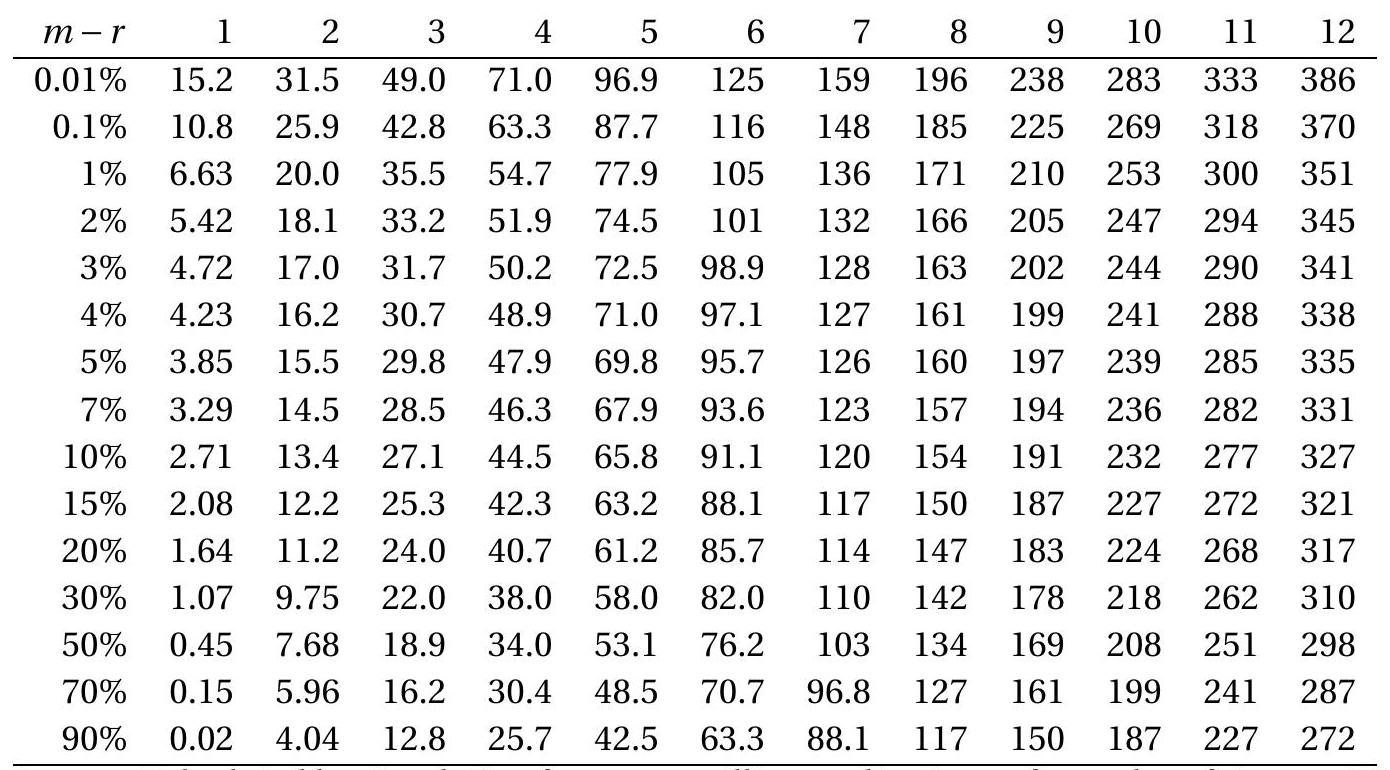
\includegraphics[max width=\textwidth]{2022_10_23_e99fc7c58db661c6f219g-41}

Source: Calculated by simulation from one million replications of samples of size $n=10,000$.

Theorem $16.22$ provides the asymptotic distribution of the LR test for cointegration rank. Because the asymptotic distribution equals the trace of a multivariate Dickey-Fuller distribution the statistic LR is often referred to as the "trace test" or "Johansen's trace test". The asymptotic distribution is a function of the stochastic process $X(r)$ which equals the trend components of $Y_{t}$ (under the hypothesis of $r$ cointegrating vectors) projected orthogonal to the other regressors. For Trend Model 2 the intercept is included in the cointegrating relationship so it is a component of $X(r)$. For Trend Model 3 the variables are trended which dominates the other components so appears in the asymptotic distribution. Since the intercept is excluded from the cointegrating relationship the components of $X(r)$ are all demeaned. For Trend Model 4 the linear trend is included in the cointegrating relationship so it is added to the trend components while the intercept is excluded so the $X(r)$ process is demeaned.

The asymptotic distribution is a function only of $m-r$ and the trend specification. Asymptotic critical values ${ }^{18}$ are displayed in Tables $16.6$-16.8 for $m-r$ up to 12 for Trend Models 2, 3, and 4. These are upper-tailed tests, so the null hypothesis that the cointegrating rank is $r$ is rejected if the test statistic is larger than the appropriate critical value; otherwise the null hypothesis is nor rejected. For example, the hypothesis of no cointegration is the same as $r=0$. The appropriate critical value is then the column corresponding to the number of variables $m$. For example, for Trend Model 2 with $m=4$ variables the $5 \%$ critical value is 54.1. If $\operatorname{LR}(r)>54.1$ the hypothesis of no coingration is rejected (implying that the series are cointegrated); otherwise the hypothesis of no cointegration is not rejected.

How are the test statistics $\operatorname{LR}(r)$ used in practice? When the cointegrating rank is unknown the statistics can be used to determine $r$. The conventional procedure is a sequential test. Start with $\mathbb{H}(0)$ (the null hypothesis of no cointegration) and the associated statistic LR(0) which has $m$ degrees of freedom. If the test rejects (if LR(0) exceeds the row $m$ critical value) this is evidence that there is at least one cointegrating vector, or $r \geq 1$. Next, take $\mathbb{\square}(1)$ (the null hypothesis of one cointegrating vector) and the associated statistic LR(1) which has $m-1$ degrees of freedom. If this test also rejects (if LR(1) exceeds the row $m-1$ critical value) this is evidence that there is at least two cointegrating vectors, or $r \geq 2$. Continue this sequence of tests until one fails to reject.

For example, when there are two variables $(m=2)$ compare the statistic $\operatorname{LR}(0)$ against the $m=2$ critical value. If the test rejects (if the statistic exceeds the critical value) this is evidence that the series are cointegrated. If the test fails to reject the inference is uncertain.

Table 16.8: VECM Cointegration Rank Critical Values: Trend Model 4

\begin{tabular}{rrrrrrrrrrrrr}
$m-r$ & 1 & 2 & 3 & 4 & 5 & 6 & 7 & 8 & 9 & 10 & 11 & 12 \\
\hline
$0.01 \%$ & $27.4$ & $44.4$ & $64.6$ & $90.0$ & 117 & 150 & 186 & 226 & 271 & 319 & 372 & 428 \\
$0.1 \%$ & $22.1$ & $38.1$ & $57.4$ & $81.0$ & 108 & 139 & 175 & 214 & 258 & 305 & 356 & 412 \\
$1 \%$ & $16.6$ & $31.2$ & $49.4$ & $71.5$ & $97.6$ & 128 & 162 & 200 & 242 & 288 & 338 & 392 \\
$2 \%$ & $14.9$ & $29.0$ & $46.7$ & $68.4$ & $94.0$ & 124 & 157 & 195 & 236 & 282 & 332 & 385 \\
$3 \%$ & $13.9$ & $27.6$ & $45.1$ & $66.4$ & $91.8$ & 121 & 154 & 192 & 233 & 278 & 328 & 381 \\
$4 \%$ & $13.1$ & $26.7$ & $43.9$ & $65.0$ & $90.1$ & 119 & 152 & 189 & 230 & 275 & 325 & 378 \\
$5 \%$ & $12.5$ & $25.9$ & $42.9$ & $63.9$ & $88.8$ & 118 & 151 & 187 & 228 & 273 & 322 & 375 \\
$7 \%$ & $11.7$ & $24.7$ & $41.4$ & $62.1$ & $86.7$ & 115 & 148 & 184 & 225 & 270 & 318 & 371 \\
$10 \%$ & $10.7$ & $23.3$ & $39.8$ & $60.1$ & $84.4$ & 113 & 145 & 181 & 221 & 266 & 314 & 366 \\
$15 \%$ & $9.53$ & $21.7$ & $37.7$ & $57.6$ & $81.5$ & 109 & 141 & 177 & 217 & 261 & 309 & 360 \\
$20 \%$ & $8.70$ & $20.5$ & $36.2$ & $55.7$ & $79.2$ & 107 & 138 & 174 & 213 & 257 & 304 & 356 \\
$30 \%$ & $7.45$ & $18.7$ & $33.8$ & $52.8$ & $75.7$ & 103 & 134 & 169 & 207 & 250 & 297 & 348 \\
$50 \%$ & $5.70$ & $15.9$ & $30.0$ & $48.1$ & $70.2$ & $96.2$ & 126 & 160 & 198 & 240 & 286 & 336 \\
$70 \%$ & $4.28$ & $13.5$ & $26.7$ & $43.8$ & $65.0$ & $90.1$ & 119 & 152 & 189 & 231 & 276 & 325 \\
$90 \%$ & $2.79$ & $10.5$ & $22.4$ & $38.2$ & $58.0$ & $81.8$ & 110 & 141 & 177 & 217 & 261 & 309 \\
\hline
\end{tabular}

Source: Calculated by simulation from one million replications of samples of size $n=10,000$.

This testing procedure is appealing when $m$ is small (e.g. $m \leq 4$ ) but is less appealing for large $m$.

${ }^{18}$ Calculated by simulation from one million simulation draws for a sample of size $n=10,000$. With large $m$ the procedure has several challenges. Sequential testing requires multiple testing for which it is difficult to control Type I error. Simultaneously the test can have low power implying that the procedure is likely to "identify" an inappropriately low value of $r$.

An alternative approach is to use cointegration tests to verify a selected specification. Start with economic modeling to motivate the cointegrating rank $r$. The likelihood ratio $\operatorname{LR}(r)$ can be used to test this assumption against the unrestricted VAR. If the test rejects $\mathbb{H}(r)$ this is evidence that the proposed model is incorrect.

We illustrate using the interest rate series with a $\operatorname{VAR}(4)$ and Trend Model 2. Our starting presumption is that the variables are $I(1)$ and cointegrated, implying that the cointegrating rank is $r=1$. The value of LR(0) is 31.6. To compute the $\mathrm{p}$-value we use Table $16.6$ for Trend Model 2 with $m-r=2$. The value $31.6$ exceeds the $1 \%$ critical value of $25.1$ so the asymptotic $p$-value of the test is less than $1 \%$. Thus the null hypothesis of no cointegration is strongly rejected in favor of at least one cointegrating vector. The value of $\operatorname{LR}(1)$ is $2.8$. The $\mathrm{p}$-value is calculated using $m-r=1$. The value $2.8$ is smaller than the $50 \%$ critical value of $3.5$ so the p-value is larger than $50 \%$. The statistic does not reject the hypothesis of $\mathbb{\square}(1)$. Together the statistics are consistent with the modeling assumption that the series are $I(1)$ and mutually cointegrated.

For a broader application we expand to five Treasury interest rates ${ }^{19}: 3$-month, 6-month, 1-year, 5-year, and 10-year. Our starting presumption is that the series are each $I(1)$ and that the system of variables are cointegrated, so that the cointegrating rank is at least one. If all four spreads are mutually stationary then the system will have four coingrating vectors, thus $r=4$. However if the the distribution of the spreads change over time the cointegrating rank could be less than four. Thus we expect $1 \leq r \leq 4$ but are uncertain of its precise value.

We report the likelihood ratio tests for cointegration rank in Table 16.9. The LR test for $r=0$ is 120 which exceeds the $1 \%$ critical value of $85.4$, and the LR test for $r=1$ is $68.3$ which exceeds the $1 \%$ critical value of $61.3$, so we safely reject the hypotheses of $r=0$ and $r=1$. This suggests that $r \geq 2$. The LR test for $r=2$ is $33.6$ with a p-value of $0.07$, which is borderline significant. The tests for $r=3$ and $r=4$ are insignificant. In sum, we cannot reject the models $\mathbb{H}(2), \mathbb{H}(3)$, or $\mathbb{H}(4) . \mathbb{H}(2)$ is doubtful, but the statistical evidence alone cannot distinguish $\mathbb{M}(3)$ versus $\mathbb{M}(4)$. Our recommendation in this context is to use either $\mathbb{H}(3)$ or $\mathbb{H}(4)$

Table 16.9: Tests for Cointegrating Rank

\begin{tabular}{ccc}
\hline\hline
 & LR(r) & p-value \\
\cline { 2 - 3 }
0 & 120 & $<0.01$ \\
1 & $68.3$ & $<0.01$ \\
2 & $33.6$ & $0.07$ \\
3 & $10.8$ & $>0.50$ \\
4 & $2.9$ & $>0.50$ \\
\hline
\end{tabular}

In Stata use vecrank to calculate the LR tests for cointegrating rank. The output is a table displaying $\mathrm{LR}(\mathrm{r})$ for $r=0, \ldots, m-1$ along with the asymptotic $5 \%$ critical values. The p-value can be calculated from Tables 16.6-16.8.

${ }^{19}$ FRED-MD series TB3MS, TB6MS, GS1, GS5, and GS10.

\subsection{Technical Proofs*}
Proof of Theorem 16.1. In the text we showed that the limit distributions of $S_{n}$ coincide with those of $B$. To appeal to the Functional Central Limit Theorem (Theorem $18.3$ of Probability and Statistics for Economists) we need to verify that $S_{n}$ is asymptotically equicontinuous (see Definition $18.7$ of Probability and Statistics for Economists). For simplicity we focus on the scalar case $e_{t} \in \mathbb{R}$. that

Assume without loss of generality that $\sigma^{2}=1$. Take any $0<\eta<1$ and $0<\epsilon<1$. Set $\delta \leq \epsilon \eta^{4} / 48^{2}$. Note
$$
\sup _{\left|r_{2}-r_{1}\right| \leq \delta}\left|S_{n}\left(r_{2}\right)-S_{n}\left(r_{1}\right)\right| \leq 2 \sup _{0 \leq j \leq\lfloor 1 / \delta\rfloor} \sup _{0 \leq r \leq \delta}\left|S_{n}(j \delta+r)-S_{n}(j \delta)\right| .
$$
Then
$$
\begin{aligned}
\mathbb{P}\left[\sup _{\left|r_{2}-r_{1}\right| \leq \delta}\left|S_{n}\left(r_{2}\right)-S_{n}\left(r_{1}\right)\right|>\eta\right] & \leq \mathbb{P}\left[\bigcup_{j=0}^{\lfloor 1 / \delta\rfloor} \sup _{0 \leq r \leq \delta}\left|S_{n}(j \delta+r)-S_{n}(j \delta)\right|>\frac{\eta}{2}\right] \\
& \leq \sum_{j=0}^{\lfloor 1 / \delta\rfloor} \mathbb{P}\left[\sup _{0 \leq r \leq \delta}\left|S_{n}(j \delta+r)-S_{n}(j \delta)\right|>\frac{\eta}{2}\right] \\
& \leq\left(\frac{1}{\delta}+1\right) \mathbb{P}\left[\sup _{0 \leq r \leq \delta}\left|S_{n}(r)\right|>\frac{\eta}{2}\right] \\
&=\left(\frac{1}{\delta}+1\right) \mathbb{P}\left[\max _{i \leq\lfloor n \delta\rfloor}\left|\frac{1}{\sqrt{n}} \sum_{t=1}^{i} e_{t}\right|>\frac{\eta}{2}\right] \\
& \leq 2\left(\frac{1}{\delta}+1\right) \mathbb{P}\left[\left|\frac{1}{\sqrt{n}} \sum_{t=1}^{\lfloor n \delta\rfloor} e_{t}\right|>\frac{\eta}{4}\right] .
\end{aligned}
$$
The final inequality is Billingsley's (B.52) which holds because $\delta<\eta / 4 \sqrt{2}$ under the assumptions. Our statement (B.52) of Billingsley's inequality assumes that $e_{t}$ is an i.i.d. sequence; the result can be extended to a MDS sequence. by

The CLT implies that $n^{-1 / 2} \sum_{t=1}^{\lfloor n \delta\rfloor} e_{t} \underset{d}{\rightarrow} Z_{\delta} \sim \mathrm{N}(0, \delta)$. For $n$ sufficiently large the final line is bounded
$$
\frac{3}{\delta} \mathbb{P}\left[\left|Z_{\delta}\right|>\frac{\eta}{4}\right]=\frac{3}{\delta} \mathbb{P}\left[Z_{\delta}^{4}>\frac{\eta^{4}}{16^{2}}\right] \leq \frac{3}{\delta} \frac{16^{2}}{\eta^{4}} \mathbb{E}\left[Z^{4}\right]=\frac{48^{2}}{\eta^{4}} \delta=\epsilon .
$$
The first inequality is Markov's, the following equality $\mathbb{E}\left[Z_{\delta}^{4}\right]=3 \delta^{2}$, and the final equality is the assumption $\delta=\epsilon \eta^{4} / 48^{2}$. This shows that $S_{n}$ satisfies the definition of asymptotic equicontinuity.

Proof of Theorem 16.7. $Z_{t}$ has the Wold decomposition $Z_{t}=\Theta(\mathrm{L}) e_{t}$. We add the additional assumption that $e_{t}$ is a MDS to simplify the proof. By the Beveridge-Nelson decomposition $Z_{t}=\xi_{t}+U_{t}-U_{t-1}$ where $\xi_{t}=\Theta(1) e_{t}$ and $U_{t}=\Theta^{*}(\mathrm{~L}) e_{t}$. Then
$$
\begin{aligned}
\frac{1}{n} \sum_{t=1}^{n} S_{t-1} Z_{t}^{\prime} &=\frac{1}{n} \sum_{t=1}^{n} S_{t-1} \xi_{t}^{\prime}+\frac{1}{n} \sum_{t=1}^{n} S_{t-1} U_{t}^{\prime}-\frac{1}{n} \sum_{t=1}^{n} S_{t-1} U_{t-1}^{\prime} \\
&=\frac{1}{n} \sum_{t=1}^{n} S_{t-1} \xi_{t}^{\prime}-\frac{1}{n} \sum_{t=1}^{n-1} Z_{t} U_{t}^{\prime}+o_{p}(1) .
\end{aligned}
$$
The first term converges to $\int_{0}^{1} B d B^{\prime}$ by Theorem 16.6. The Brownian motion has covariance matrix equal to the long-run variance of $Z_{t}$, which is $\Omega$. The second term converges in probability to $\mathbb{E}\left[Z_{t} U_{t}^{\prime}\right]$. Making the substitutions $U_{t}=\xi_{t+1}+U_{t+1}-Z_{t+1}$ and $\mathbb{E}\left[Z_{t} \xi_{t+1}^{\prime}\right]=0$ this can be written as
$$
\begin{aligned}
\mathbb{E}\left[Z_{t} U_{t}^{\prime}\right] &=\mathbb{E}\left[Z_{t} \xi_{t+1}^{\prime}\right]+\mathbb{E}\left[Z_{t} U_{t+1}^{\prime}\right]-\mathbb{E}\left[Z_{t} Z_{t+1}^{\prime}\right] \\
&=\mathbb{E}\left[Z_{t} U_{t+1}^{\prime}\right]-\mathbb{E}\left[Z_{t} Z_{t+1}^{\prime}\right] \\
&=\mathbb{E}\left[Z_{t} U_{t+2}^{\prime}\right]-\mathbb{E}\left[Z_{t} Z_{t+2}^{\prime}\right]-\mathbb{E}\left[Z_{t} Z_{t+1}^{\prime}\right] \\
&=\cdots \\
&=-\sum_{j=1}^{\infty} \mathbb{E}\left[Z_{t} Z_{t+j}^{\prime}\right]=-\sum_{j=1}^{\infty} \mathbb{E}\left[Z_{t-j} Z_{t}^{\prime}\right]=-\Lambda .
\end{aligned}
$$
The third line makes the substitutions $U_{t+1}=\xi_{t+2}+U_{t+2}-Z_{t+2}$ and $\mathbb{E}\left[Z_{t} \xi_{t+2}^{\prime}\right]=0$, and the substitutions are repeated until infinity. We have shown the result as claimed.

Proof of Theorem 16.8. By the definition of the stochastic integral
$$
\int_{0}^{1} W d W=\operatorname{plim}_{N \rightarrow \infty} \sum_{i=0}^{N-1} W\left(\frac{i}{N}\right)\left(W\left(\frac{i+1}{N}\right)-W\left(\frac{i}{N}\right)\right) .
$$
Take any positive integer $N$ and any $j<N$. Observe that
$$
W\left(\frac{j+1}{N}\right)=W\left(\frac{j}{N}\right)+\left(W\left(\frac{j+1}{N}\right)-W\left(\frac{j}{N}\right)\right) .
$$
Squaring we obtain
$$
W\left(\frac{j+1}{N}\right)^{2}-W\left(\frac{j}{N}\right)^{2}=2 W\left(\frac{j}{N}\right)\left(W\left(\frac{j+1}{N}\right)-W\left(\frac{j}{N}\right)\right)+\frac{1}{N} \chi_{j N} .
$$
where $\chi_{j N}=N\left(W\left(\frac{j+1}{N}\right)-W\left(\frac{j}{N}\right)\right)^{2}$. Notice that $\chi_{j N}$ are i.i.d. across $j$, distributed as $\chi_{1}^{2}$, and have expectation 1. Summing over $j=0$ to $N-1$ we obtain
$$
W(1)^{2}=2 \sum_{i=0}^{N-1} W\left(\frac{i}{N}\right)\left(W\left(\frac{i+1}{N}\right)-W\left(\frac{i}{N}\right)\right)+\frac{1}{N} \sum_{i=0}^{N-1} \chi_{i N}^{2} .
$$
Rewriting
$$
\sum_{i=0}^{N-1} W\left(\frac{i}{N}\right)\left(W\left(\frac{i+1}{N}\right)-W\left(\frac{i}{N}\right)\right)=\frac{1}{2}\left(W(1)^{2}-\frac{1}{N} \sum_{i=0}^{N-1} \chi_{i N}^{2}\right) .
$$
By (16.26), $\int_{0}^{1} W d W$ is the probability limit of the right side. By the WLLN this is $\frac{1}{2}\left(W(1)^{2}-1\right)$ as claimed.

Proof of Theorem 16.10.
$$
\widehat{\sigma}^{2}=\frac{1}{n} \sum_{t=1}^{n-1} \widehat{e}_{t+t}^{2}=\frac{1}{n} \sum_{t=1}^{n-1} e_{t+t}^{2}-\frac{1}{n} \frac{\left(\frac{1}{n} \sum_{t=1}^{n-1} Y_{t} e_{t+1}\right)^{2}}{\frac{1}{n^{2}} \sum_{t=1}^{n-1} Y_{t}^{2}}=\frac{1}{n} \sum_{t=1}^{n-1} e_{t+t}^{2}+o_{p}(1) \longrightarrow \vec{p}^{2} .
$$
Then
$$
T=\frac{\frac{1}{n} \sum_{t=1}^{n-1} Y_{t} e_{t+1}}{\left(\frac{1}{n^{2}} \sum_{t=1}^{n-1} Y_{t}^{2}\right)^{1 / 2}} \underset{\widehat{\sigma}}{\longrightarrow} \frac{\sigma^{2} \int_{0}^{1} W d W}{\left(\sigma^{2} \int_{0}^{1} W^{2}\right)^{1 / 2} \sigma}=\frac{\int_{0}^{1} W d W}{\left(\int_{0}^{1} W^{2}\right)^{1 / 2}}
$$
Proof of Theorem 16.12. Pick $\eta>0$ and $\epsilon>0$. Pick $\delta$ such that
$$
\mathbb{P}\left(\sup _{|r-s| \leq \delta}|X(r)-X(s)|>\epsilon\right) \leq \eta
$$
which is possible since $X(r)$ is almost surely continuous. Set $N=\lfloor 1 / \delta\rfloor$ and $t_{k}=k n / N$. Write $X_{n t}=$ $D_{n}^{-1} X_{t}$. Then
$$
C_{n}=\frac{1}{n} \sum_{k=0}^{N} \sum_{t=t_{k}}^{t_{k+1}-1} X_{n t} u_{t}=\frac{1}{n} \sum_{k=0}^{N} X_{n, t_{k}} \sum_{t=t_{k}}^{t_{k+1}-1} u_{t}+\frac{1}{n} \sum_{k=0}^{N} \sum_{t=t_{k}}^{t_{k+1}-1}\left(X_{n t}-X_{n, t_{k}}\right) u_{t}
$$
and
$$
\left|C_{n}\right| \leq \sup _{0 \leq r \leq 1}\left|X_{n}(r)\right| A_{n}+\sup _{|r-s| \leq \delta}\left|X_{n}(r)-X_{n}(s)\right| B_{n}
$$
where
$$
\begin{aligned}
&A_{n}=\frac{N}{n} \max _{k \leq N}\left|\sum_{t=t_{k}}^{t_{k+1}-1} u_{t}\right| \\
&B_{n}=\frac{1}{n} \sum_{t=1}^{n}\left|u_{t}\right| .
\end{aligned}
$$
Since $X_{n} \underset{d}{\longrightarrow} X$ and $X$ is continuous,
$$
\sup _{0 \leq r \leq 1}\left|X_{n}(r)\right| \underset{d}{\longrightarrow} \sup _{0 \leq r \leq 1}|X(r)|<\infty
$$
almost surely. Thus $\sup _{0 \leq r \leq 1}\left|X_{n}(r)\right|=O_{p}(1)$. Since $X_{n} \underset{d}{\longrightarrow} X$,
$$
\sup _{|r-s| \leq \delta}\left|X_{n}(r)-X_{n}(s)\right| \underset{d}{\longrightarrow} \sup _{|r-s| \leq \delta}|X(r)-X(s)| \leq \epsilon
$$
where the inequality holds with probability exceeding $1-\eta$ by (16.27). Thus for sufficiently large $n$ the left hand side is bounded by $2 \epsilon$ with the same probability, and hence is $o_{p}(1)$.

For fixed $N, A_{n} \underset{p}{\longrightarrow} 0$ by the ergodic theorem. The assumption that $\mathbb{E}\left|u_{t}\right|<\infty$ implies that $B_{n}=O_{p}(1)$. Together, we have shown that
$$
\left|C_{n}\right| \leq O_{p}(1) o_{p}(1)+o_{p}(1) O_{p}(1)=o_{p}(1)
$$
as stated.

Proof of Theorem 16.17.

Part 1: The definition of cointegration implies that $\Delta Y_{t}$ is stationary with a finite covariance matrix. By the multivariate Wold representation (Theorem 15.2), $\Delta Y_{t}=\theta+\Theta(\mathrm{L}) e_{t}$ with the errors white noise. Premultiplication by $\beta^{\prime}$ yields $\beta^{\prime} \Delta Y_{t}=\beta^{\prime} \theta+\beta^{\prime} \Theta(\mathrm{L}) e_{t}$ which has long-run variance $\beta^{\prime} \Theta(1) \Sigma \Theta(1)^{\prime} \beta$ where $\Sigma$ is the covariance matrix of $e_{t}$. The assumption that $\beta^{\prime} Y_{t}$ is $I(0)$ implies that $\beta^{\prime} \theta=0$ (else $\beta^{\prime} Y_{t}$ will have a time trend). This implies $\theta$ lies in the range space of $\beta_{\perp}$, hence $\theta=\beta_{\perp} \gamma$ for some $\gamma$. Also, the assumption that $\beta^{\prime} Y_{t}$ is $I(0)$ implies that $\beta^{\prime} \Delta Y_{t}$ is $I(-1)$, which implies that its long-run covariance matrix equals zero. This implies that $\beta^{\prime} \Theta(1)=0$ and hence $\Theta(1)=\beta_{\perp} \eta^{\prime}$ for some matrix $\eta$. The assumption that $\beta_{\perp}^{\prime} \Delta Y_{t}$ is $I(0)$ implies that $\beta_{\perp}^{\prime} \Theta(1) \Sigma \Theta(1)^{\prime} \beta_{\perp}>0$ which implies that $\Theta(1)$ must have rank $m-r$ and hence so does the matrix $\eta$

Part 2: The Beveridge-Nelson decomposition plus $\Theta(1)=\beta_{\perp} \eta^{\prime}$ implies $\Theta(\mathrm{L})=\beta_{\perp} \eta^{\prime}+\Theta^{*}(\mathrm{~L})(1-\mathrm{L})$. Applied to the Wold representation we obtain $\Delta Y_{t}=\beta_{\perp} \gamma+\beta_{\perp} \eta^{\prime} e_{t}+\Theta^{*}(\mathrm{~L}) \Delta e_{t}$. Summing we find the stated representation.

Part 3: Without loss of generality assume that $H=\left[\beta, \beta_{\perp}\right]$ is orthonormal. Also define the orthonormal matrix $H_{\eta}=\left[\eta_{\perp}, \bar{\eta}\right]$ where $\bar{\eta}=\eta\left(\eta^{\prime} \eta\right)^{-1 / 2}$. Define $X_{t}=H^{\prime} Y_{t}$. The Wold representation implies $\Delta X_{t}=$ $\left(\begin{array}{l}0 \\ \gamma\end{array}\right)+C(\mathrm{~L}) e_{t}$ where using the Beveridge-Nelson decomposition
$$
\boldsymbol{C}(\mathrm{L})=H^{\prime}\left(\beta_{\perp} \eta^{\prime}+\Theta^{*}(\mathrm{~L})(1-\mathrm{L})\right)=\left(\begin{array}{c}
\beta^{\prime} \Theta^{*}(\mathrm{~L})(1-\mathrm{L}) \\
\eta^{\prime}+\beta_{\perp}^{\prime} \Theta^{*}(\mathrm{~L})(1-\mathrm{L})
\end{array}\right)
$$
Partition $X_{t}=\left(X_{1 t}, X_{2 t}\right)$ comformably with $H$. We see that
$$
\left(\begin{array}{c}
\Delta X_{1 t} \\
\Delta X_{2 t}
\end{array}\right)=\left(\begin{array}{c}
\beta^{\prime} \Theta^{*}(\mathrm{~L})(1-\mathrm{L}) e_{t} \\
\gamma+\eta^{\prime} e_{t}+\beta_{\perp}^{\prime} \Theta^{*}(\mathrm{~L})(1-\mathrm{L}) e_{t}
\end{array}\right) .
$$
Summing the first equation we obtain
$$
\left(\begin{array}{c}
X_{1 t} \\
\Delta X_{2 t}
\end{array}\right)=\left(\begin{array}{c}
\mu \\
\gamma
\end{array}\right)+\boldsymbol{D}(\mathrm{L}) H_{\eta}^{\prime} e_{t}
$$
where $\mu=X_{1,0}-\beta^{\prime} \Theta^{*}(\mathrm{~L}) e_{0}$ and
$$
\boldsymbol{D}(\mathrm{L})=\left(\begin{array}{c}
\beta^{\prime} \Theta^{*}(\mathrm{~L}) \\
\eta^{\prime}+\beta_{\perp}^{\prime} \Theta^{*}(\mathrm{~L})(1-\mathrm{L})
\end{array}\right) H_{\eta}=\left(\begin{array}{cc}
\beta^{\prime} \Theta^{*}(\mathrm{~L}) \eta_{\perp} & \beta^{\prime} \Theta^{*}(\mathrm{~L}) \bar{\eta} \\
\beta_{\perp}^{\prime} \Theta^{*}(\mathrm{~L}) \eta_{\perp}(1-\mathrm{L}) & \left(\eta^{\prime} \eta\right)^{1 / 2}+\beta_{\perp}^{\prime} \Theta^{*}(\mathrm{~L}) \bar{\eta}(1-\mathrm{L})
\end{array}\right) .
$$
This is an invertible matrix polynomial. To see this, first observe that
$$
\boldsymbol{D}(1)=\left(\begin{array}{cc}
\beta^{\prime} \Theta^{*}(1) \eta_{\perp} & \beta^{\prime} \Theta^{*}(1) \bar{\eta} \\
0 & \left(\eta^{\prime} \eta\right)^{1 / 2}
\end{array}\right)
$$
which is full rank under the assumption that $\beta^{\prime} \Theta^{*}(1) \eta_{\perp}$ is full rank. This means that $\operatorname{det}(\boldsymbol{D}(z))$ has no unit roots. Second, (16.28) and the definition of $X_{t}$ imply that
$$
\boldsymbol{D}(z)=\left(\begin{array}{cc}
1-z & 0 \\
0 & 1
\end{array}\right) H \Theta(z) H_{\eta} .
$$
Since $H$ and $H_{\eta}$ are full rank this implies that the solutions to $\operatorname{det}(\boldsymbol{D}(z))=0$ are solutions to $\operatorname{det}(\Theta(z))=0$ and hence satisfy $|z| \geq 1+\delta$ (because $z \neq 1$ ) by the assumption on $\Theta(z)$. Together we have shown that $\boldsymbol{D}(\mathrm{L})$ is invertible. Thus (16.28) implies
$$
H_{\eta} \boldsymbol{D}(\mathrm{L})^{-1}\left(\begin{array}{c}
X_{1 t} \\
\Delta X_{2 t}
\end{array}\right)=a+e_{t}
$$
where
$$
a=H_{\eta} \boldsymbol{D}(1)^{-1}\left(\begin{array}{l}
\mu \\
\gamma
\end{array}\right) \text {. }
$$
(16.29) is a VAR representation for $\left(\beta^{\prime} Y_{t}, \beta_{\perp}^{\prime} \Delta Y_{t}\right)$ with all roots satisfying $|z| \geq 1+\delta$. This implies a VAR representation for $Y_{t}$ which is equation (16.18) with
$$
\boldsymbol{A}(z)=H_{\eta} \boldsymbol{D}(z)^{-1}\left(\begin{array}{c}
\beta^{\prime} \\
\beta_{\perp}^{\prime}(1-z)
\end{array}\right) .
$$
By partitioned matrix inversion we calculate
$$
\begin{aligned}
\boldsymbol{A}(1) &=H_{\eta} \boldsymbol{D}(1)^{-1}\left(\begin{array}{c}
\beta^{\prime} \\
0
\end{array}\right) \\
&=\left[\eta_{\perp}, \bar{\eta}\right]\left(\begin{array}{cc}
\left(\beta^{\prime} \Theta^{*}(1) \eta_{\perp}\right)^{-1} & -\left(\beta^{\prime} \Theta^{*}(1) \eta_{\perp}\right)^{-1} \beta^{\prime} \Theta^{*}(1) \eta \\
0 & \left(\eta^{\prime} \eta\right)^{-1 / 2}
\end{array}\right)\left(\begin{array}{c}
\beta^{\prime} \\
0
\end{array}\right) \\
&=\eta_{\perp}\left(\beta^{\prime} \Theta^{*}(1) \eta_{\perp}\right)^{-1} \beta^{\prime} \\
&=-\alpha \beta^{\prime} .
\end{aligned}
$$
as claimed.

Part 4. Under the assumption $\sum_{j=0}^{\infty}\left\|\sum_{k=0}^{\infty} k \Theta_{j+k}\right\|^{2}<\infty$, Theorem $15.3$ implies that the coefficients $\boldsymbol{A}_{k}^{*}=$ $\sum_{j=0}^{\infty} \boldsymbol{A}_{j+k}$ are absolutely summable. We can then apply the Beveridge-Nelson decomposition $\boldsymbol{A}(z)=$ $\boldsymbol{A}(1)+\boldsymbol{A}^{*}(z)(1-z)$. Applying $\boldsymbol{A}(1)=-\alpha \beta^{\prime}$ and a little rewriting yields
$$
\boldsymbol{A}(z)=\boldsymbol{I}_{m}(1-z)-\alpha \beta^{\prime} z-\left(\boldsymbol{I}_{m}+\alpha \beta^{\prime}-\boldsymbol{A}^{*}(z)\right)(1-z) .
$$
Applied to (16.18) we obtain the stated result with $\Gamma(\mathrm{L})=\boldsymbol{I}_{m}+\alpha \beta^{\prime}-A^{*}(z)$. The coefficients of $\Gamma(\mathrm{L})$ are absolutely summable because the coefficients $\boldsymbol{A}_{k}^{*}$ are.

Part 5. The assumption $\theta=0$ direct implies $\gamma=0$. This implies
$$
\begin{aligned}
a &=H_{\eta} \boldsymbol{D}(1)^{-1}\left(\begin{array}{c}
\mu \\
0
\end{array}\right) \\
&=\left[\eta_{\perp}, \bar{\eta}\right]\left(\begin{array}{cc}
\left(\beta^{\prime} \Theta^{*}(1) \eta_{\perp}\right)^{-1} & -\left(\beta^{\prime} \Theta^{*}(1) \eta_{\perp}\right)^{-1} \beta^{\prime} \Theta^{*}(1) \eta \\
0 & \left(\eta^{\prime} \eta\right)^{-1 / 2}
\end{array}\right)\left(\begin{array}{c}
\mu \\
0
\end{array}\right) \\
&=\eta_{\perp}\left(\beta^{\prime} \Theta^{*}(1) \eta_{\perp}\right)^{-1} \mu \\
&=\alpha \mu
\end{aligned}
$$
as claimed.

Proof of Theorem 16.18. Write the VECM as $\Gamma^{*}(\mathrm{~L}) \Delta Y_{t}-\alpha \beta^{\prime} Y_{t-1}=a+e_{t}$ where $\Gamma^{*}(z)=\boldsymbol{I}_{m}-\Gamma(z)$. Set $\bar{\alpha}=\alpha\left(\alpha^{\prime} \alpha\right)^{-1 / 2}$ and orthonormal $H=\left[\bar{\alpha}, \alpha_{\perp}\right]$. Assume that $\left[\beta, \beta_{\perp}\right]$ is orthonormal. Define $Z_{t}=\beta^{\prime} Y_{t}$ and $U_{t}=\beta_{\perp}^{\prime} \Delta Y_{t}$. Our goal is to show that $\left(Z_{t}, U_{t}\right)$ is $I(0)$ which is the same as showing that $Y_{t}$ is cointegrated with cointegrating vectors $\beta$.

Premultiplying the VECM model by $H^{\prime}$ we find the system
$$
H^{\prime}\left(\Gamma^{*}(\mathrm{~L}) \Delta Y_{t}-\alpha \beta^{\prime} Y_{t-1}\right)=H^{\prime} a+H^{\prime} e_{t} .
$$
Using the identity $\boldsymbol{I}_{m}=\beta \beta^{\prime}+\beta_{\perp} \beta_{\perp}^{\prime}$ we see that $\Delta Y_{t}=\beta \Delta Z_{t}+\beta_{\perp} U_{t}$. Making this substitution and setting $\bar{a}=H^{\prime} a v_{t}=H^{\prime} e_{t}$ we obtain the system
$$
\boldsymbol{D}(\mathrm{L})\left(\begin{array}{c}
Z_{t} \\
U_{t}
\end{array}\right)=\bar{a}+v_{t}
$$
where
$$
\boldsymbol{D}(z)=\left[\begin{array}{cc}
\bar{\alpha}^{\prime} \Gamma^{*}(z) \beta(1-z)-\boldsymbol{I}_{m} & \bar{\alpha}^{\prime} \Gamma^{*}(z) \beta_{\perp} \\
\alpha_{\perp}^{\prime} \Gamma^{*}(z) \beta(1-z) & \alpha_{\perp}^{\prime} \Gamma^{*}(z) \beta_{\perp}
\end{array}\right] .
$$
We now show that this is a stationary system. First, note that
$$
\boldsymbol{D}(1)=\left[\begin{array}{cc}
-\boldsymbol{I}_{m} & \bar{\alpha}^{\prime} \Gamma^{*}(1) \beta_{\perp} \\
0 & \alpha_{\perp}^{\prime} \Gamma^{*}(1) \beta_{\perp}
\end{array}\right]
$$
which is full rank under the assumption that $\alpha_{\perp}^{\prime} \Gamma^{*}(1) \beta_{\perp}$ is full rank. That means that $\operatorname{det}(\boldsymbol{D}(z))=0$ has no solutions $z=1$. Second, $\boldsymbol{D}(z)$ relates to $\boldsymbol{A}(z)$ by the relationship
$$
\boldsymbol{D}(z)=H^{\prime} \boldsymbol{A}(z)\left[\beta, \beta_{\perp}(1-z)\right] .
$$
Thus the solutions $z \neq 1$ to
$$
\operatorname{det}(\boldsymbol{D}(z))=\operatorname{det}(H) \operatorname{det}(\boldsymbol{A}(z)) \operatorname{det}\left(\left[\beta, \beta_{\perp}(1-z)\right]\right)=0
$$
are all solutions to $\operatorname{det}(\boldsymbol{A}(z))=0$, which all satisfy $|z| \geq 1+\delta$ by assumption. Thus $\boldsymbol{D}(z)$ is invertible with summable moving average coefficient matrices. This implies the VAR system for $\left(Z_{t}, U_{t}\right)$ is stationary.

As discussed above, this shows that $\left(Z_{t}, U_{t}\right)$ is a stationary process and hence $Y_{t}$ is cointegrated with cointegrating vector $\beta$.

Proof of Theorem 16.19. Set $Y_{2 t}^{*}=Y_{2 t}-\bar{Y}_{2}$. The estimator satisfies
$$
n(\widehat{\beta}-\beta)=\left(\frac{1}{n^{2}} \sum_{t=1}^{n} Y_{2 t}^{*} Y_{2 t}^{* \prime}\right)^{-1}\left(\frac{1}{n} \sum_{t=1}^{n} Y_{2 t}^{*} u_{1 t}\right)
$$
Set $S_{t}=\sum_{i=1}^{t} u_{t}$. Theorems $16.4$ and $16.5$ imply $S_{\lfloor n r\rfloor} \underset{d}{\longrightarrow} B(r)$ and $Y_{2\lfloor n r\rfloor}^{*} \underset{d}{\longrightarrow} B_{2}^{*}(r)$. By the continuous mapping theorem
$$
\frac{1}{n^{2}} \sum_{t=1}^{n} Y_{2 t}^{*} Y_{2 t}^{* \prime} \underset{d}{\longrightarrow} \int_{0}^{1} B_{2}^{*} B_{2}^{* \prime} \text {. }
$$
By Theorem $16.7$ and the WLLN
$$
\frac{1}{n} \sum_{t=1}^{n} Y_{2 t}^{*} u_{1 t}=\frac{1}{n} \sum_{t=1}^{n} Y_{2 t-1}^{*} u_{1 t}+\frac{1}{n} \sum_{t=1}^{n} u_{2 t} u_{1 t}+o_{p}(1) \underset{d}{\longrightarrow} \int_{0}^{1} B_{2}^{*} d B_{1}+\Lambda_{21}+\Sigma_{21} .
$$
Together we obtain the stated result.

Proof of Theorem $16.22$ (sketch). For simplicity abstract from the dynamic and trend coefficients so that the unconstrained model is
$$
\Delta Y_{t}=\alpha \beta^{\prime} Y_{t-1}+e_{t} .
$$
where $e_{t}$ is a MDS with covariance matrix $\Sigma$. We examine two cases in detail. First, the case $\mathbb{R}(0)$ (which is relatively straightforward) and second the case $\mathbb{H}(r)$ (which is algebraically more tedious).

First, take $\mathbb{H}(0)$, in which case the process is $\Delta Y_{t}=e_{t}$. The statistic is
$$
\begin{aligned}
\operatorname{LR}(0) &=-n \sum_{j=1}^{m} \log \left(1-\hat{\lambda}_{j}\right) \simeq n \sum_{j=1}^{m} \widehat{\lambda}_{j} \\
&=\operatorname{tr}\left[\left(\frac{1}{n} \sum_{t=1}^{n} Y_{t-1} e_{t}^{\prime}\right)\left(\frac{1}{n} \sum_{t=1}^{n} e_{t} e_{t}^{\prime}\right)^{-1}\left(\frac{1}{n} \sum_{t=1}^{n} e_{t} Y_{t-1}^{\prime}\right)\left(\frac{1}{n^{2}} \sum_{t=1}^{n} Y_{t-1} Y_{t-1}^{\prime}\right)^{-1}\right] \\
& \underset{d}{\rightarrow} \operatorname{tr}\left[\left(\int_{0}^{1} d B B^{\prime}\right)\left(\int_{0}^{1} B B^{\prime}\right)^{-1}\left(\int_{0}^{1} B d B^{\prime}\right)\right] \\
&=\operatorname{tr}\left[\left(\int_{0}^{1} d W W^{\prime}\right)\left(\int_{0}^{1} W W^{\prime}\right)^{-1}\left(\int_{0}^{1} W d W^{\prime}\right)\right]
\end{aligned}
$$
where $B(r)$ is a Brownian motion with covariance matrix $\Sigma$, and $W(r)=\Sigma^{-1 / 2} B(r)$ is standard Brownian motion. This is the stated result. Second, take $\mathbb{H}(r)$ for $1<r<m$. Define $Z_{t}=\beta^{\prime} Y_{t}$. The process under $\mathbb{H}(r)$ is $\Delta Y_{t}=\alpha Z_{t-1}+e_{t}$. Normalize $\beta$ so that $\mathbb{E}\left[Z_{t} Z_{t}^{\prime}\right]=\boldsymbol{I}_{r}$. The test statistic is invariant to linear transformations of $Y_{t}$ so we can rescale the data so that $\mathbb{E}\left[\Delta Y_{t} \Delta Y_{t}^{\prime}\right]=\boldsymbol{I}_{m}$. Notice that $\Sigma=\mathbb{E}\left[e_{t} e_{t}^{\prime}\right]=\mathbb{E}\left[\Delta Y_{t} \Delta Y_{t}^{\prime}\right]-\alpha \mathbb{E}\left[Z_{t} Z_{t}^{\prime}\right] \alpha^{\prime}=\boldsymbol{I}_{m}-\alpha \alpha^{\prime}$.

The likelihood ratio statistic is
$$
\operatorname{LR}(r)=-n \sum_{j=r+1}^{m} \log \left(1-\widehat{\lambda}_{j}\right) \simeq \sum_{j=r+1}^{m} \widehat{\rho}_{j}
$$
where $\widehat{\rho}_{j}=n \widehat{\lambda}_{j}$ are the $m-r$ smallest roots of the equation $\operatorname{det}(S(\rho))=0$ where
$$
S(\rho)=\rho \frac{1}{n^{2}} \sum_{t=1}^{n} Y_{t-1} Y_{t-1}^{\prime}-\frac{1}{n} \sum_{t=1}^{n} Y_{t-1} \Delta Y_{t}^{\prime}\left(\frac{1}{n} \sum_{t=1}^{n} \Delta Y_{t} \Delta Y_{t}^{\prime}\right)^{-1} \frac{1}{n} \sum_{t=1}^{n} \Delta Y_{t} Y_{t-1}^{\prime} .
$$
Define a full-rank matrix $H=\left[\beta, \beta_{\perp}\right]$ where $\beta^{\prime} \beta_{\perp}=0$. The roots of $\widehat{\rho}_{j}$ are the same as those of $\operatorname{det}\left(S^{*}(\rho)\right)=$ 0 where $S^{*}(\rho)=H^{\prime} S(\rho) H$, which replaces $Y_{t-1}$ with $\left(Z_{t-1}, X_{t-1}\right)$ where $X_{t}=\beta_{\perp}^{\prime} Y_{t}$. We calculate that
$$
\begin{aligned}
S^{*}(\rho) &=\rho\left[\begin{array}{cc}
\frac{1}{n^{2}} \sum_{t=1}^{n} Z_{t-1} Z_{t-1}^{\prime} & \frac{1}{n^{2}} \sum_{t=1}^{n} Z_{t-1} X_{t-1}^{\prime} \\
\frac{1}{n^{2}} \sum_{t=1}^{n} X_{t-1} Z_{t-1}^{\prime} & \frac{1}{n^{2}} \sum_{t=1}^{n} X_{t-1} X_{t-1}^{\prime}
\end{array}\right] \\
&-\left[\begin{array}{c}
\frac{1}{n} \sum_{t=1}^{n} Z_{t-1} \Delta Y_{t}^{\prime} \\
\frac{1}{n} \sum_{t=1}^{n} X_{t-1} \Delta Y_{t}^{\prime}
\end{array}\right]\left(\frac{1}{n} \sum_{t=1}^{n} \Delta Y_{t} \Delta Y_{t}^{\prime}\right)^{-1}\left[\begin{array}{c}
\frac{1}{n} \sum_{t=1}^{n} Z_{t-1} \Delta Y_{t}^{\prime} \\
\frac{1}{n} \sum_{t=1}^{n} X_{t-1} \Delta Y_{t}^{\prime}
\end{array}\right]^{\prime} .
\end{aligned}
$$
We now apply the asymptotic theory for non-stationary theory to each component. The process $X_{t}=$ $\beta_{\perp}^{\prime} Y_{t}$ is non-stationary and satisfies the FCLT $n^{-1} X_{\lfloor n r\rfloor} \underset{d}{\longrightarrow} X(r) \sim B M\left(\beta_{\perp}^{\prime} \Omega \beta_{\perp}\right)$ where $\Omega$ is the long-run covariance matrix of $\Delta Y_{t}$. The sum of the errors satisfy $n^{-1 / 2} \sum_{t=1}^{\lfloor n r\rfloor} e_{t} \underset{d}{\longrightarrow} B(r) \sim B M(\Sigma)$. The process $X(r)$ is a linear function of $B(r)$.

We find that $\frac{1}{n^{2}} \sum_{t=1}^{n} X_{t-1} X_{t-1}^{\prime} \underset{d}{\longrightarrow} \int_{0}^{1} X X^{\prime}, \frac{1}{n^{2}} \sum_{t=1}^{n} X_{t-1} e_{t} \underset{d}{\longrightarrow} \int_{0}^{1} X d B^{\prime}, \frac{1}{n} \sum_{t=1}^{n} Z_{t-1} Z_{t-1}^{\prime} \underset{p}{\longrightarrow} \boldsymbol{I}_{r}, \frac{1}{n} \sum_{t=1}^{n} \Delta Y_{t} \Delta Y_{t}^{\prime} \underset{p}{\longrightarrow}$ $\boldsymbol{I}_{m}, \frac{1}{n} \sum_{t=1}^{n} Z_{t-1} \Delta Y_{t}^{\prime} \underset{p}{\longrightarrow} \alpha^{\prime}, \frac{1}{n} \sum_{t=1}^{n} X_{t-1} Z_{t-1}^{\prime} \underset{d}{\longrightarrow} \zeta$ for some random matrix by Theorem 16.7, and $\frac{1}{n} \sum_{t=1}^{n} X_{t-1} \Delta Y_{t}^{\prime} \underset{d}{\longrightarrow}$ $\zeta^{\prime} \alpha^{\prime}+\int_{0}^{1} X d B^{\prime}$. Together we find that
$$
S^{*}(\rho) \underset{d}{\longrightarrow} \rho\left[\begin{array}{cc}
0 & \\
0 & \int_{0}^{1} X X^{\prime}
\end{array}\right]-\left[\begin{array}{cc}
\alpha^{\prime} \alpha & \alpha^{\prime}\left(\alpha \zeta+\int_{0}^{1} d B X^{\prime}\right) \\
\left(\zeta^{\prime} \alpha^{\prime}+\int_{0}^{1} X d B^{\prime}\right) \alpha & \left(\zeta^{\prime} \alpha^{\prime}+\int_{0}^{1} X d B^{\prime}\right)\left(\alpha \zeta+\int_{0}^{1} d B X^{\prime}\right)
\end{array}\right] .
$$
Thus $\operatorname{det}\left(S^{*}(\rho)\right)$ converges in distribution to the determinant of the right-hand-side, which equals (using Theorem A.1.5) $\operatorname{det}\left(\alpha^{\prime} \alpha\right)$ multiplied by the determinant of
$$
\begin{aligned}
&\rho \int_{0}^{1} X X^{\prime}-\left(\zeta^{\prime} \alpha^{\prime}+\int_{0}^{1} X d B^{\prime}\right)\left(I_{m}-\alpha\left(\alpha^{\prime} \alpha\right)^{-1} \alpha^{\prime}\right)\left(\alpha \zeta+\int_{0}^{1} d B X^{\prime}\right) \\
&=\rho \int_{0}^{1} X X^{\prime}-\int_{0}^{1} X d B^{\prime} M_{\alpha} \int_{0}^{1} d B X^{\prime} \\
&=\rho \int_{0}^{1} X X^{\prime}-\int_{0}^{1} X d W^{\prime} H_{1}^{\prime} \int_{0}^{1} H_{1} d W X^{\prime} \\
&=\rho \int_{0}^{1} X X^{\prime}-\int_{0}^{1} X d W^{\prime} \int_{0}^{1} d W X^{\prime}
\end{aligned}
$$
where $M_{\alpha}=\boldsymbol{I}_{m}-\alpha\left(\alpha^{\prime} \alpha\right)^{-1} \alpha^{\prime}$ and
$$
M_{\alpha} B(r) \sim B M\left(M_{\alpha}\left(\boldsymbol{I}_{m}-\alpha \alpha^{\prime}\right) M_{\alpha}\right)=B M\left(M_{\alpha}\right)=H_{1} W(r)
$$
where $M_{\alpha}=H_{1} H_{1}^{\prime}, H_{1}^{\prime} H_{1}=\boldsymbol{I}_{m-r}$ and $W(r) \sim B M\left(\boldsymbol{I}_{m-r}\right)$.

The determinant of (16.30) has $m-r$ roots and their sum equals
$$
\operatorname{tr}\left[\left(\int_{0}^{1} d W X^{\prime}\right)\left(\int_{0}^{1} X X^{\prime}\right)^{-1}\left(\int_{0}^{1} X d W^{\prime}\right)\right]=\operatorname{tr}\left[\left(\int_{0}^{1} d W W^{\prime}\right)\left(\int_{0}^{1} W W^{\prime}\right)^{-1}\left(\int_{0}^{1} W d W^{\prime}\right)\right]
$$
because $X(r)$ is a linear rotation of $W(r)$. This is the stated result.

\subsection{Exercises}
Exercise 16.1 Take $S_{t}=S_{t-1}+e_{t}$ with $S_{0}=0$ and $e_{t}$ i.i.d. $\left(0, \sigma^{2}\right)$.

(a) Calculate $\mathbb{E}\left[S_{t}\right]$ and $\operatorname{var}\left[S_{t}\right]$.

(b) Set $Y_{t}=\left(S_{t}-\mathbb{E}\left[S_{t}\right]\right) / \sqrt{\operatorname{var}\left[S_{t}\right]}$. By construction $\mathbb{E}\left[Y_{t}\right]=0$ and $\operatorname{var}\left[Y_{t}\right]=1$. Is $Y_{t}$ stationary?

(c) Find the asymptotic distribution of $Y_{\lfloor n r\rfloor}$ for $r \in[\delta, 1]$.

Exercise 16.2 Find the Beveridge-Nelson decomposition of $\Delta Y_{t}=e_{t}+\Theta_{1} e_{t-1}+\Theta_{2} e_{t-2}$.

Exercise 16.3 Suppose $Y_{t}=X_{t}+u_{t}$ where $X_{t}=X_{t-1}+e_{t}$ with $\left(e_{t}, u_{t}\right) \sim I(0)$.

(a) Is $Y_{t} I(0)$ or $I(1)$ ?.

(b) Find the asymptotic functional distribution of $\mathrm{n}^{-1 / 2} Y_{\lfloor n r\rfloor}$.

Exercise 16.4 Let $Y_{t}=e_{t}$ be i.i.d. and $X_{t}=\Delta Y_{t}$.

(a) Show that $Y_{t}$ is stationary and $I(0)$.

(b) Show that $X_{t}$ is stationary but not $I(0)$.

Exercise 16.5 Let $U_{t}=U_{t-1}+e_{t}, Y_{t}=U_{t}+v_{t}$ and $X_{t}=2 U_{t}+w_{t}$, where $\left(e_{t}, v_{t}, w_{t}\right)$ is an i.i.d. sequence. Find the cointegrating vector for $\left(Y_{t}, X_{t}\right)$.

Exercise 16.6 Take the AR(1) model $Y_{t}=\alpha Y_{t-1}+e_{t}$ with i.i.d. $e_{t}$ and the least squares estimator $\widehat{\alpha}$. In Chaper 14 we learned that the asymptotic distribution when $|\alpha|<1$ is $\sqrt{n}(\widehat{\alpha}-\alpha) \underset{d}{\longrightarrow} \mathrm{N}\left(0,1-\alpha^{2}\right)$. How do you reconcile this with Theorem $16.9$, especially for $\alpha$ close to one?

Exercise 16.7 Take the VECM(1) model $\Delta Y_{t}=\alpha \beta^{\prime} Y_{t-1}+e_{t}$. Show that $Z_{t}=\beta^{\prime} Y_{t}$ follows an AR(1) process.

Exercise 16.8 An economist estimates the model $Y_{t}=\alpha Y_{t-1}+e_{t}$ and finds $\widehat{\alpha}=0.9$ with $s(\widehat{\alpha})=0.05$. They assert: "The t-statistic for testing $\alpha=1$ is 2 , so $\alpha=1$ is rejected." Is there an error in their reasoning?

Exercise 16.9 An economist estimates the model $Y_{t}=\alpha Y_{t-1}+e_{t}$ and finds $\widehat{\alpha}=0.9$ with $s(\widehat{\alpha})=0.04$. They assert: "The $95 \%$ confidence interval for $\alpha$ is $[0.82,0.98]$ which does not contain 1 . So $\alpha=1$ is not consistent with the data." Is there an error in their reasoning?

Exercise 16.10 An economist takes $Y_{t}$, detrends to obtain the detrended series $Z_{t}$, applies a ADF test to $Z_{t}$ and finds $\mathrm{ADF}=-2.5$. They assert: "Stata provides the $5 \%$ critical value $-1.9$ with $\mathrm{p}$-value less than $1 \%$. Thus we reject the null hypothesis of a unit root." Is there an error in their reasoning? Exercise 16.11 An economist wants to build an autoregressive model for the number of daily tweets by a prominant politician. For a model with an intercept they obtain $\mathrm{ADF}=-2.0$. They assert "The number of tweets is a unit root process." Is there an error in their reasoning?

Exercise 16.12 For each of the following monthly series from FRED-MD implement the Dickey-Fuller unit root test. For each, you need to consider the AR order $p$ and the trend specification.

(a) log real personal income: $\log (r p i)$

(b) industrial production index: indpro

(c) housing starts: houst

(d) help-wanted index: hwi

(e) civilian labor force: clf16ov

(f) initial claims: claims

(g) industrial production index (fuels): ipfuels

Exercise 16.13 For each of the series in the previous exercise implement the KPSS test of stationarity. For each, you need consider the lag truncation $M$ and the trend specification.

Exercise 16.14 For each of the following monthly pairs from FRED-MD test the hypothesis of no cointegration using the Johansen trace test. For each, you need to consider the VAR order $p$ and the trend specification.

(a) 3-month treasury interest rate $(t b 3 m s)$ and 10-year treasury interest rate $(g s 10)$. Note: In the text we implemented the test on the quarterly series, not monthly.

(b) interest rate on AAA bonds $(a a a)$ and interest rate on BAA bonds $(b a a)$.

(c) $\log ($ industrial production durable consumer goods) and log(industrial production nondurable consumer goods) (log of ipdcongd and ipncongd).


\end{document}